\chapter{Interacci'on del campo electromagn'etico cuantizado con la
materia.}

\section{Interacci'on del campo electromagn'etico cl'asico con la
materia}
\subsection{Lagrangeano cl'asico}
El lagrangeano de una part'icula (no-relativista) de masa $m$ y carga $q$
movi'endose en un campo electromagn'etico, es dado por 
\begin{equation}
L=\frac{1}{2}m\dot{\vec{x}}^2+\frac{q}{c}\vec{A}\cdot \dot{\vec{x}}-q\varphi ,
\label{lagc}
\end{equation}
donde $\vec{A}=\vec{A}\left( \vec{x},t\right) $ y $\varphi =\varphi
\left( \vec{x},t\right) $ son el potencial vectorial y escalar del campo
electromagn'etico en la posici'on $\vec{x}$ y el instante $t$.

El momentum conjugado $\vec{p}$ es dado por 
\begin{equation}
\vec{p}=\frac{\partial L}{\partial
\dot{\vec{x}}}=m\dot{\vec{x}}+\frac{q}{c}\vec{A} \label{pc},
\end{equation}
y las ecuaciones de Lagrange nos dirigen a 
\begin{equation}
m \ddot{\vec{x}}=q\left( \vec{E}+\frac{1}{c}\dot{\vec{x}}\times
\vec{B}\right) .
\end{equation}

En efecto,
\begin{equation}
\frac{\partial L}{\partial x_i} =q\left( \frac{1}{c}\dot{x}_{j}\partial
_iA_{j}-\partial _i\varphi \right),
\end{equation} 
\begin{equation}
\frac{d}{dt}\frac{\partial L}{\partial \dot{x}_i}=\frac{d}{dt}\left( m\dot{%
x}_i+\frac{q}{c}A_i\right) ,
\end{equation}
de modo que las ecuaciones de Euler-Lagrange son:
\begin{eqnarray}
\frac{q}{c}\partial _iA_{j}\dot{x}_{j}-q\partial _i\varphi -\frac{d}{dt}%
\left( m\dot{x}_i+\frac{q}{c}A_i\right) &=&0 ,\\
\frac{q}{c}\partial _iA_{j}\dot{x}_{j}-q\partial _i\varphi -m\ddot{x}_i-%
\frac{q}{c}\frac{d}{dt}A_i &=&0 ,\\
\frac{q}{c}\partial _iA_{j}\dot{x}_{j}-q\partial _i\varphi -\frac{q}{c}%
\frac{d}{dt}A_i &=&m\ddot{x}_i,
\end{eqnarray}
pero $\frac{d}{dt}=\frac{\partial }{\partial t}+\dot{x}_k\partial _k$, de
modo que obtenemos
\begin{eqnarray}
\frac{q}{c}\partial _iA_{j}\dot{x}_{j}-q\partial _i\varphi -\frac{q}{c}%
\frac{\partial }{\partial t}A_i-\frac{q}{c}\dot{x}_k\partial _kA_i
&=&m\ddot{x}_i, \\
\frac{q}{c}\left( \partial _iA_{j}\dot{x}_{j}-\dot{x}_k\partial
_kA_i\right) +q\left( -\partial _i\varphi -\frac{1}{c}\frac{\partial }{%
\partial t}A_i\right) &=&m\ddot{x}_i.
\end{eqnarray}
Recordando las expresiones del campo el'ectrico y magn'etico en funci'on de los
potenciales:
\begin{eqnarray}
E_i &=&-\partial _i\varphi -\frac{1}{c}\frac{\partial A_i}{\partial t}, \\
B_i &=&\varepsilon _{ijk}\partial _{j}A_k,
\end{eqnarray}
tenemos 
\begin{eqnarray}
\frac{q}{c}\dot{x}_{j}\left( \partial _iA_{j}-\partial _{j}A_i\right)
+qE_i &=&m\ddot{x}_i, \\
\frac{q}{c}\dot{x}_{j}\left( \delta _{mi}\delta _{jn}-\delta _{mj}\delta
_{in}\right) \partial _{m}A_{n}+qE_i &=&m\ddot{x}_i ,\\
\frac{q}{c}\dot{x}_{j}\varepsilon _{kij}\varepsilon _{kmn}\partial
_{m}A_{n}+qE_i &=&m\ddot{x}_i ,\\
\frac{q}{c}\varepsilon _{kij}\dot{x}_{j}B_k+qE_i &=&m\ddot{x}_i ,\\
\frac{q}{c}\varepsilon _{ijk}\dot{x}_{j}B_k+qE_i &=&m\ddot{x}_i .
\end{eqnarray}
De modo que obtenemos finalmente
\begin{equation}
m\ddot{x}_i=q\left( E_i+\frac{1}{c}\varepsilon _{ijk}\dot{x}%
_{j}B_k\right) . 
\end{equation}


\subsection{Hamiltoniano cl'asico} 

El Hamiltoniano est'a dado por la transformada de Legendre del Lagrangiano:  
\begin{equation}
H=\vec{p}\cdot \dot{\vec{x}}-L .
\end{equation}
Usando (\ref{lagc}) y (\ref{pc}), encontramos
\begin{eqnarray}
H &=&\vec{p}\cdot \dot{\vec{x}}-\left( \frac{1}{2}m\dot{\vec{x}}%
^2+\frac{q}{c}\vec{A}\cdot \dot{\vec{x}}-q\varphi \right) \\
&=&\vec{p}\cdot \dot{\vec{x}}-\frac{1}{2}m\dot{\vec{x}}^2-\frac{q%
}{c}\vec{A}\cdot \dot{\vec{x}}+q\varphi \\
&=&\vec{p}\cdot \dot{\vec{x}}-\frac{q}{c}\vec{A}\cdot
\dot{\vec{x}}-\frac{1}{2}m\dot{\vec{x}}^2+q\varphi \\
&=&\left( \vec{p}-\frac{q}{c}\vec{A}\right) \cdot \dot{\vec{x}}-%
\frac{1}{2}m\dot{\vec{x}}^2+q\varphi \\
&=&\left( \vec{p}-\frac{q}{c}\vec{A}\right) \cdot \frac{1}{m}\left( 
\vec{p}-\frac{q}{c}\vec{A}\right) -\frac{1}{2}m\frac{1}{m^2}\left( 
\vec{p}-\frac{q}{c}\vec{A}\right)^2+q\varphi \\
&=&\frac{1}{m}\left( \vec{p}-\frac{q}{c}\vec{A}\right)^2-\frac{1}{2m%
}\left( \vec{p}-\frac{q}{c}\vec{A}\right)^2+q\varphi \\
&=&\frac{1}{2m}\left( \vec{p}-\frac{q}{c}\vec{A}\right)^2+q\varphi .
\end{eqnarray}
As'i, finalmente obtenemos
\begin{equation}
H=H_{\rm libre}+H_{\rm int},
\end{equation} 
donde $H_{\rm libre}:=\frac{1}{2m} p^2$ es el hamiltoniano de una part'icula
(no-relativista) libre, y
\begin{equation}\label{Hintnorel}
H_{\rm int} =-\frac{q}{mc}\,\vec{p}\cdot\vec{A}
+\frac{q^2}{2mc^2}\,\vec{A}^2+q\varphi ,
\end{equation} 
es el hamiltoniano de interacci'on con el campo electromagn'etico.

\subsection{Interacci'on de una part'icula no-relativista con el campo
electromagn'etico cu'antico}

Describimos las propiedades cu'anticas de una part'icula de masa $m$ y carga $q$
interactuando con el campo electromag'etico cuantizado por medio del
hamiltoniano total
\begin{eqnarray}
\hat{H}&=& \hat{H}_{\rm libre}+\hat{H}'+\hat{H}''+\hat{H}_{\hat{\varphi}}
+\hat{H}_{\rm rad} \label{hatH}\\
&=&\frac{1}{2m} \hat{\vec{p}}\,^2-\frac{q}{2mc}\,\left(
\hat{\vec{p}}\cdot\hat{\vec{A}}+\hat{\vec{A}}\cdot\hat{\vec{p}}\right)
+\frac{q^2}{2mc^2}\,\hat{\vec{A}}{\,}^2+q\hat{\varphi}+ \frac{1}{8\pi}\int dV
(\hat{E}^2+\hat{B}^2) ,
\end{eqnarray} 
donde $\hat{\vec{p}}$ es el operador momentum de la part'icula, que satisface
las usuales relaciones de conmutaci'on usadas en la mec'anica cu'antica de una
part'icula, es decir, $\left[ \vec{x}_i,\vec{p}_j\right]
=i\hbar\delta_{i,j}\hat{1}$ (en la
representaci'on coordenada $\vec{p}_j=-i\hbar \partial_j$)	, y
$(\hat{\varphi},\hat{\vec{A}})$ son los campos cu'anticos que describen el campo
electromagn'etico. Adem'as, hemos dividido los t'erminos del hamiltoniano de
interacci'on en
\begin{eqnarray}
\hat{H}'&:=&-\frac{q}{2mc}\,\left(
\hat{\vec{p}}\cdot\hat{\vec{A}}+\hat{\vec{A}}\cdot\hat{\vec{p}}\right),\\
\hat{H}''&:=&\frac{q^2}{2mc^2}\,\hat{\vec{A}}{\,}^2, \\
\hat{H}_{\hat{\varphi}}&:=&q\hat{\varphi} .
\end{eqnarray} 
En el gauge de Coulomb, s'olo $\hat{H}'$ y $\hat{H}''$ contribuyen a la
interacci'on. Adem'as,
$\hat{\vec{p}}\cdot\hat{\vec{A}}-\hat{\vec{A}}\cdot\hat{\vec{p}}=-i\hbar(\vec{
\nabla}\cdot \hat{\vec{A}}) \hat{1}=0$ (cuando act'uan sobre un vector del
espacio de Hilbert). Finalmente, el operador $\hat{\vec{A}}$ que describe el
campo electromagn'etico cuantizado (libre) tiene la forma (\ref{Afi}), de modo
que
\begin{eqnarray}
\hat{H}'&=&-\frac{e}{mc}\sqrt{\frac{2\pi\hbar
c^2}{L^3}}\sum_{\vec{k},\sigma}\frac{\hat{\vec{p}}\cdot\check{\varepsilon
}_{\vec{k}\sigma}}{\sqrt{\omega_k}}\left\{ \hat{a}_{\vec{k}\sigma}%
e^{i\vec{k}\cdot\vec{x}}+\hat{a}_{\vec{k}\sigma}^\dagger e^{-i\vec{k}%
\cdot\vec{x}}\right\} \label{H1},\\
\hat{H}''&=&\frac{e^2}{2mc^2}\left( \frac{2\pi\hbar
c^2}{L^3}\right)
\sum_{\vec{k},\sigma}\sum_{\vec{k}',\sigma'}\frac{\check{\varepsilon}_{\vec{k}
\sigma}\cdot\check{\varepsilon}_{\vec{k}'\sigma
'}}{\sqrt{\omega_k\omega_{k'}}}\left\{\hat{a}_{\vec{k}\sigma}\hat{a}_{\vec{k}
'\sigma '}e^{i\left( \vec{k}+\vec{k}'\right)
\cdot\vec{x}}+\hat{a}_{\vec{k}\sigma}\hat{a}_{\vec{k}'\sigma
'}^\dagger e^{i\left( \vec{k}-\vec{k}'\right) \cdot\vec{x}}\right. \nonumber \\
&&\left.+\hat{a}_{\vec{k}\sigma}^\dagger \hat{a}_{\vec{k}'\sigma '}e^{-i\left(
\vec{k}-\vec{k}'\right)
\cdot\vec{x}}+\hat{a}_{\vec{k}\sigma}^\dagger \hat{a}_{\vec{k}'\sigma
'}^\dagger e^{-i\left( \vec{k}+\vec{k}'\right) \cdot\vec{x}}\right\}
.\label{H2}
\end{eqnarray} 

Para la evaluaci'on de los diferentes procesos usaremos teor'ia de
perturbaciones (dependiente del tiempo), tomando como hamiltoniano ``modelo'' a
\begin{equation}
\hat{H}_0=\hat{H}_{\rm libre}+\hat{H}_{\rm rad}, \label{H0}
\end{equation} 
que ya sabemos diagonalizar. Como base del sistema part'icula + campo
consideraremos a estados de la forma $\left|\Psi\right\rangle \left|\cdots
n_{\vec{k},\sigma}\cdots\right\rangle $. Los hamiltonianos de interacci'on
$\hat{H}'$ y
$\hat{H}''$ son entonces considerados como perturbaciones.

Es ilustrativo preguntarse cu'al es el par'ametro adimensional (y peque\~no) que
usaremos para definir la serie perturbativa de un proceso dado. Para esto,
reescribiremos $\hat{H}'$ y $\hat{H}''$ en funci'on de cantidades
adimensionales:
\begin{eqnarray}
\frac{1}{mc^2}\hat{H}'&=&-\sqrt{\frac{e^2}{\hbar
c}}\sum_{\vec{k},\sigma}\sqrt{\frac{c\lambda_c^2}{2\pi  L^3\omega_k}}\left(
\frac{\hat{\vec{p}}}{mc}\right) \cdot\check{\varepsilon
}_{\vec{k}\sigma}\left\{ \hat{a}_{\vec{k}\sigma}%
e^{i\vec{k}\cdot\vec{x}}+\hat{a}_{\vec{k}\sigma}^\dagger e^{-i\vec{k}%
\cdot\vec{x}}\right\} ,\\
\frac{1}{mc^2}\hat{H}''&=&\frac{1}{2}\left( \frac{e^2}{\hbar c }\right) 
\sum_{\vec{k},\sigma}\sum_{\vec{k}',\sigma'}\left( \frac{c\lambda_c^2}{2\pi
L^3\sqrt{\omega_k\omega_{k'}}}
\right)\check{\varepsilon}_{\vec{k}\sigma}\cdot\check{\varepsilon}_{\vec{k}
'\sigma '}\left\{\hat{a}_{\vec{k}\sigma}\hat{a}_{\vec{k}'\sigma '}e^{i\left(
\vec{k}+\vec{k}'\right) \cdot\vec{x}}\right. \nonumber \\
&&\left.++\hat{a}_{\vec{k}\sigma}\hat{a}_{\vec{k}'\sigma '}^\dagger e^{i\left(
\vec{k}-\vec{k}'\right)
\cdot\vec{x}}\hat{a}_{\vec{k}\sigma}^\dagger \hat{a}_{\vec{k}'\sigma
'}e^{-i\left( \vec{k}-\vec{k}'\right)
\cdot\vec{x}}+\hat{a}_{\vec{k}\sigma}^\dagger \hat{a}_{\vec{k}'\sigma
'}^\dagger e^{-i\left( \vec{k}+\vec{k}'\right) \cdot\vec{x}}\right\}.
\end{eqnarray} 
Aqu'i hemos reemplazado $q=e$ ($e<0$ para un electr'on). Esta expresi'on
implica que, si medimos momentum en unidades de $mc$, frecuencia en unidades
de $\frac{c\lambda_c^2}{2\pi L^3}$ (donde
$\lambda_c:=\frac{h}{mc}=\frac{2\pi\hbar}{mc}$ es la longitud de Compton del
electr'on o, en general, de la part'icula) y  energ'ia en unidades de $mc^2$,
entonces la magnitud de la interacci'on es proporcional a la \textit{constante
de structura fina} $\alpha:=\frac{e^2}{\hbar c}\approx \frac{1}{137}$, con
$\hat{H}'\sim O(\sqrt{\alpha}$) y $\hat{H}''\sim O(\alpha)$. Podemos adoptar a
$\alpha$ como el par'ametro adimensional ($\ll 1$) con respecto al cual
calcularemos nuestra expansi'on perturbativa. Debido a que $\alpha\propto e^2$,
la serie perturbativa puede considerarse formalmente en potencias de la carga
$e$, con $\hat{H}'\sim O(e)$ y $\hat{H}''\sim O(e^2)$.

\subsection{Teor'ia de Perturbaciones y regla de oro de Fermi}

Regla de Oro de Fermi: La probabilidad por unidad de tiempo que ocurra la
transici'on entre el estado inicial $\left| i\right\rangle $ y el estado final
$\left|
f\right\rangle $ de un sistema cu'antico, es
\begin{equation}
\left( \frac{P}{t}\right)=\frac{2\pi}{\hbar}\left|
M_{\rm fi}\right|^2\delta\left( E_f%
-E_i\right) ,\label{Fermi Rule}%
\end{equation}
donde $M_{\rm fi}$ es la \textit{matriz de transici'on} dada por:%
\begin{equation}
M_{\rm fi}:=\left\langle f\right| \hat{H}_{int}\left| i\right\rangle 
+\sum_{I}\frac{\left\langle f\right| \hat{H}_{int}\left|
I\right\rangle  \left\langle I\right| \hat{H}_{int}\left|
i\right\rangle  }{E_i-E_{I}}+\sum_{I,II}\frac{\left\langle f\right|
\hat{H}_{int}\left| I\right\rangle  \left\langle I\right| \hat{H}%
_{int}\left| II\right\rangle  \left\langle II\right| \hat{H}%
_{int}\left| i\right\rangle  }{\left( E_i-E_{I}\right) \left(
E_i-E_{II}\right) }+\dots,\label{Mfi(1)}%
\end{equation}
con $\left| I\right\rangle  $ y $\left| II\right\rangle  $ todos los
posibles estados intermedios del sistema. 

En nuestro caso tenemos que el hamiltoniano de interacci'on es de la forma
\begin{equation}
\hat{H}_{int}=\hat{H}'+\hat{H}'' .\label{Hint}%
\end{equation}
Al reemplazar (\ref{Hint}) en (\ref{Mfi(1)}), encontramos que la matriz de
puede escribirse como:%
\begin{eqnarray}
M_{\rm fi} & = &\left\langle f\right| \left( \hat{H}'+\hat{H}''\right)
\left| i\right\rangle  +\sum_{I}\frac{\left\langle f\right| \left(
\hat{H}'+\hat{H}''\right) \left| I\right\rangle  \left\langle
I\right| \left( \hat{H}'+\hat{H}''\right) \left|i\right\rangle  }{E_i-E_{I}}\\
&& +\sum_{I,II}\frac{\left\langle f\right| \left( \hat
{H}'+\hat{H}''\right) \left| I\right\rangle  \left\langle
I\right| \left( \hat{H}'+\hat{H}''\right) \left|
II\right\rangle  \left\langle II\right| \left( \hat{H}'+\hat
{H}''\right) \left| i\right\rangle  }{\left( E_i-E_{I}\right) \left(
E_i-E_{II}\right) }+\dots\\
& = &\left\langle f\right| \hat{H}'\left| i\right\rangle 
+\left\langle f\right| \hat{H}''\left| i\right\rangle 
+\sum_{I}\frac{\left\langle f\right| \hat{H}'\left|
I\right\rangle  \left\langle I\right| \hat{H}'\left|
i\right\rangle  }{E_i-E_{I}}+\sum_{I}\frac{\left\langle f\right| \hat
{H}'\left| I\right\rangle  \left\langle I\right| \hat
{H}''\left| i\right\rangle  }{E_i-E_{I}}\\
&&+\sum_{I}\frac{\left\langle f\right| \hat{H}^{''
}\left| I\right\rangle  \left\langle I\right| \hat{H}^{'
}\left| i\right\rangle  }{E_i-E_{I}}+\sum_{I}\frac{\left\langle
f\right| \hat{H}''\left| I\right\rangle  \left\langle
I\right| \hat{H}''\left| i\right\rangle  }{E_i-E_{I}%
}+\dots
\end{eqnarray}

\section{Absorci'on de fotones por un electr'on: Contribuci'on de primer
orden en $\hat{H}'$.}

Esquem'aticamente, la absorci'on del fot'on $\vec{k}_i\sigma_i$, a primer
orden en $\hat{H}'$ corresponde al diagrama mostrado en la figura \ref{absfot}
\begin{figure}
\begin{center}
\begin{fmffile}{d1}
\begin{fmfgraph*}(50,60)
  \fmfbottom{ei,f}\fmflabel{$q_i$}{ei}\fmflabel{$k$}{f}
  \fmftop{ef}\fmflabel{$q_f$}{ef}
  \fmf{fermion}{ei,v1,ef}
  \fmf{photon}{f,v1}
 \end{fmfgraph*}
\end{fmffile}
\end{center}
\caption{Proceso de primer orden en $\hat{H}'$ para la absorci'on de un fot'on.}
\label{absfot}
\end{figure} 
En este caso, consideramos los estados iniciales y finales dados por
\begin{eqnarray}
\left| i\right\rangle  & = &\left| \vec{q}_i\right\rangle  \left|
\dots,n_{\vec{k}\sigma},\dots\right\rangle  ,\\
\left| f\right\rangle  & = &\left| \vec{q}_f\right\rangle  \left|
\dots,n_{\vec{k}\sigma}-1,\dots\right\rangle  ,
\end{eqnarray}
donde $\left| \vec{q}\right\rangle $ es un estado propio de $\hat{H}_{\rm
libre}$ de momentum definido $\hbar\vec{q}$. Tomando en cuenta las condiciones
de borde periodicas (``cuantizaci'on en la caja''), estos estados, en la
representaci'on coordenada, est'an dados por
\begin{equation}\label{OP}
\psi_{\vec{q}}\left(
\vec{x}\right) = \frac{1}{\sqrt{L^3}}e^{i\frac{\vec{p}\cdot\vec{x}}{\hbar}}=
\frac{1}{\sqrt{L^3}}e^{i\vec{q}\cdot\vec{x}},
\end{equation}
con energ'ia:%
\begin{equation}
E_{q}=\frac{\left( \hbar q\right)^2}{2m}. \label{hefree}
\end{equation}

La matriz de transici'on $M_{\rm fi}$ en este caso est'a dada, a primer orden en
$e$, por
\begin{eqnarray}
M_{\rm fi} & = &\left\langle f\right| \hat{H}'\left|
i\right\rangle  \\
& = &-\frac{e}{mc}\sqrt{\frac{2\pi\hbar c^2}{L^3}}\sum_{\vec{k}',\sigma
'}\left\langle \vec{q}_f\right| \left\langle \dots,n_{\vec{k}\sigma
}-1,\dots\right|
\frac{\hat{\vec{p}}\cdot\check{\varepsilon}_{\vec{k}'\sigma
'}}{\omega_{k'}^{1/2}}\left\{ \hat{a}_{\vec{k}'\sigma '}e^{i\vec{k}
'\cdot\vec{x}}+\hat{a}_{\vec{k}'\sigma
'}^\dagger e^{-i\vec{k}'\cdot\vec{x}}\right\} \left|
\dots,n_{\vec{k}\sigma},\dots\right\rangle 
\left| \vec{q}_i\right\rangle  \nonumber \\
& = &-\frac{e}{mc}\sqrt{\frac{2\pi\hbar c^2}{L^3}}\sum_{\vec{k}',\sigma
'}\left\{
\left\langle \dots,n_{\vec{k}\sigma}-1,\dots\right|
\hat{a}_{\vec{k}'\sigma'}\left| \dots,n_{\vec{k}\sigma},\dots\right\rangle 
\left\langle \vec{q}_f\right|
\frac{\hat{\vec{p}}\cdot\check{\varepsilon}%
_{\vec{k}'\sigma '}}{\omega_{k'}^{1/2}}e^{i\vec{k}'\cdot\vec{x}}\left|
\vec{q}_i\right\rangle  \right. \nonumber \\
&& \qquad \left.+\left\langle \dots,n_{\vec{k}\sigma}-1,\dots\right|
\hat{a}_{\vec{k}'\sigma '}^\dagger \left|
\dots,n_{\vec{k}\sigma},\dots\right\rangle 
\left\langle
\vec{q}_f\right|
\frac{\hat{\vec{p}}\cdot\check{\varepsilon}_{\vec{k}'\sigma
'}}{\omega_{k'}^{1/2}}e^{-i\vec{k}'\cdot\vec{x}}\left| \vec{q}_i\right\rangle 
\right\} \\
& = &-\frac{e}{mc}\sqrt{\frac{2\pi\hbar c^2}{L^3}}\sum_{\vec{k}',\sigma
'}\left\{\left\langle \dots,n_{\vec{k}\sigma}-1,\dots\right|
\hat{a}_{\vec{k}'\sigma '}\left|
\dots,n_{\vec{k}\sigma},\dots\right\rangle \delta_{\vec{k},\vec{k}'}\delta_{
\sigma,\sigma '}
\left\langle \vec{q}%
_f\right|\frac{\hat{\vec{p}}\cdot\check{\varepsilon}_{\vec{k}
'\sigma'}}{\omega_{k'}^{1/2}}e^{i\vec{k}'\cdot\vec{x}}\left|
\vec{q}_i\right\rangle \right\}\\
& = &-\frac{e}{mc}\sqrt{\frac{2\pi\hbar
c^2}{L^3\omega_k}}\left\{\left\langle
\dots,n_{\vec{k}\sigma}-1,\dots\right| \hat{a}_{\vec{k}\sigma}\left|
\dots,n_{\vec{k}\sigma},\dots\right\rangle  \left\langle
\vec{q}_f\right|\hat{\vec{p}}\cdot\check{\varepsilon}_{\vec{k}
\sigma}e^{i\vec{k}\cdot\vec{x}}\left|\vec{q}_i\right\rangle  \right\}\\
& = &-\frac{e}{mc}\sqrt{\frac{2\pi\hbar
c^2}{L^3\omega_k}}\left\{\sqrt{n_{\vec{k}\sigma}}\left\langle
\dots,n_{\vec{k}\sigma}-1,\dots\right|\left.
\dots,n_{\vec{k}\sigma}-1,\dots\right\rangle  \left\langle
\vec{q}_f\right|\hat{\vec{p}}\cdot\check{\varepsilon}_{\vec{k}
\sigma}e^{i\vec{k}\cdot\vec{x}}\left|\vec{q}_i\right\rangle  \right\}\\
& = &-\frac{e}{mc}\sqrt{\frac{2\pi\hbar c^2}{L^3\omega_k}}\left\langle
\vec{q}_f\right| \hat{\vec{p}}\cdot\check{\varepsilon}%
_{\vec{k}\sigma}e^{i\vec{k}\cdot\vec{x}}\left| \vec{q}_i\right\rangle 
\sqrt{n_{\vec{k}\sigma}}.
\end{eqnarray}

Por lo tanto, usando la ecuaci'on (\ref{OP}) vemos que:%
\begin{eqnarray}
\left\langle \vec{q}_f\right| \hat{\vec{p}}\cdot
\check{\varepsilon}_{\vec{k}\sigma}e^{i\vec{k}\cdot\vec{x}}\left| \vec
{q}_i\right\rangle  & \propto&\int_{V}\psi_{\vec{q}_f}^{\ast}\left(
\vec{x}\right) e^{i\vec{k}\cdot\vec{x}}\psi_{\vec{q}_i}\left( \vec
{x}\right) dV\\
& = &\int_{V}\left( \frac{1}{\sqrt{L^3}}e^{-i\vec{q}_f\cdot\vec{x}%
}\right) e^{i\vec{k}\cdot\vec{x}}\left( \frac{1}{\sqrt{L^3}}e^{i\vec
{q}_i\cdot\vec{x}}\right) dV\\
& = &\frac{1}{L^3}\int_{L^3}e^{-i\left\{ \vec{q}_f-\left( \vec{q}%
_i+\vec{k}\right) \right\} \cdot\vec{x}}dV\\
& = &\frac{1}{L^3}\left\{ L^3\delta_{\vec{q}_f,\vec{q}_i+\vec{k}%
}\right\} \\
& = &\delta_{\vec{q}_f,\vec{q}_i+\vec{k}} \, ,
\end{eqnarray}
que expresa la conservaci'on del momentum:
\begin{equation}
\hbar\vec{q}_f=\hbar\vec{q}_i+\hbar\vec{k} \, ,\label{Conservacion Momentum}
\end{equation}
mientras que de (\ref{hefree}) y de la delta en (\ref{Fermi Rule}), obtenemos la
condici'on de conservaci'on de la energ'ia:
\begin{eqnarray}
E_f & = &E_i\, ,\\
E_0+\frac{\left( \hbar\vec{q}_f\right)^2}{2m}+\hbar\omega_k\left(
n_{\vec{k}\sigma}-1\right) & = &E_0+\hbar\omega_kn_{\vec{k}\sigma}%
+\frac{\left( \hbar\vec{q}_i\right)^2}{2m} \, ,\\
% \frac{\left( \hbar\vec{q}_f\right)^2}{2m}+\hbar\omega_kn_{\vec
% {k}\sigma}-\hbar\omega_k & = &\hbar\omega_kn_{\vec{k}\sigma}+\frac{\left(
% \hbar\vec{q}_i\right)^2}{2m} \, ,\\
\frac{\left( \hbar\vec{q}_f\right)^2}{2m} & = &\hbar\omega_k%
+\frac{\left( \hbar\vec{q}_i\right)^2}{2m}.\label{Conservacion Energia}%
\end{eqnarray}

Sin embargo, es f'acil mostrar que (\ref{Conservacion Energia}) y
(\ref{Conservacion Momentum}) no pueden ser satisfechas simult'aneamente. Por lo
tanto, es imposible que un electr'on libre (aislado) absorba un fot'on. Este
resultado es v'alido tambi'en para ordenes superiores en la teor'ia de
perturbaciones.


\section{Scattering entre fotones y electrones libres.}

Consideraremos procesos de scattering del tipo mostrado en la figura
\ref{scatef}.
\begin{figure}
\begin{center}
\begin{fmffile}{d2}
\begin{fmfgraph*}(50,70)
  \fmfbottom{e1,f1}\fmflabel{$q_i$}{e1}\fmflabel{$k_i$}{f1}
  \fmftop{e2,f2}\fmflabel{$q_f$}{e2}\fmflabel{$k_f$}{f2}
  \fmfblob{0.5w}{v1}
  \fmf{fermion}{e1,v1,e2}
  \fmf{photon}{f1,v1,f2}
 \end{fmfgraph*}
\end{fmffile}
\end{center}
\caption{Scattering de fotones con electrones libres. Inicialmente un
electr'on en el estado $\left| \vec{q}_i\right\rangle  $ absorve un
fot'on $\vec{k}_i\sigma_i.$ El resultado del proceso es un fot'on
emitido $\vec{k}_f\sigma_f$ y el electr'on en el estado $\left|
\vec{q}_f\right\rangle  .$}
\label{scatef}
\end{figure} 
En este caso, consideraremos que los estados inicial y final est'an dados por
\begin{eqnarray}
\left| i\right\rangle  & = &\left| \vec{q}_i\right\rangle  \left|
\dots,n_{\vec{k}_i\sigma_i},\dots,n_{\vec{k}_f\sigma_f},\dots\right\rangle 
=\left| \vec{q}_i\right\rangle  \left| \gamma_i\right\rangle 
,\label{|i>} \\
\left| f\right\rangle  & = &\left| \vec{q}_f\right\rangle  \left|
\dots,n_{\vec{k}_i\sigma_i}-1,\dots,n_{\vec{k}_f\sigma_f}%
+1,\dots\right\rangle  =\left| \vec{q}_f\right\rangle  \left|
\gamma_f\right\rangle  .\label{|f>} 
\end{eqnarray}
En la pr'actica es conveniente describir un proceso de scattering por medio
de la correspondiente \textit{secci'on diferencial de scattering}
\begin{equation}
\frac{d\sigma}{d\Omega}:=\frac{\left( \text{N'umero de part'iculas
emitidas por unidad de tiempo y de 'angulo s'olido}\right) }{\left(
\text{N'umero de part'iculas incidentes por unidad de 'area y de
tiempo}\right)} .
\end{equation}
En el contexto de la teor'ia cu'antica, la secci'on diferencial puede
calcularse dividiendo la probabilidad por unidad de tiempo de que la part'icula
final (en nuestro caso, el fot'on final) sea emitido en el 'angulo s'olido
$d\Omega$ en la direcci'on determinada por los 'angulos de scattering
$(\vartheta,\phi)$, por la densidad de flujo de probabilidad del haz incidente:
\begin{equation}
\frac{d\sigma}{d\Omega}
d\Omega=\frac{(P/t)(\vartheta,\phi,d\Omega)}{j_0},
\end{equation}
 Note que $\frac{d\sigma}{d\Omega}$ tiene unidades de 'area. 
La densidad de flujo de probabilidad de fotones incidentes est'a dada por:
\begin{equation}
j_{0,\rm fotones}=\frac{n_{\vec{k}_i\sigma_i}}{L^3}c,
\end{equation}

De modo que
\begin{eqnarray}
d\sigma_{\vec{k},\sigma} &=&
\frac{\left(\frac{P}{t}\right)_{\text{Scattering}}}
{\frac{n_{\vec{k} _i\sigma_i}} {L^3}c}\nonumber\\
& = &\frac{2\pi L^3}{\hbar cn_{\vec{k}_i\sigma_i}}\left|
M_{\rm fi}\right|^2\delta\left( E_f-E_i\right).
\label{Seccion Transversal Absorcion}%
\end{eqnarray}
Para evaluar la matriz de transici'on, s'olo nos interesan los t'erminos que
produzcan
procesos del tipo mostrado en la figura \ref{scatef}. Estos t'erminos est'an
presentes a primer orden en $\hat{H}
''$, mientras que $\hat{H}'$ s'olo puede contribuir con t'erminos de
segundo orden en la serie perturbativa. En consecuencia, a orden $e^2$, la
matriz $M_{\rm fi}$ se reduce a:
\begin{equation}
M_{\rm fi}=\left\langle f\right| \hat{H}''\left|
i\right\rangle  +\sum_{I}\frac{\left\langle f\right| \hat{H}^{'
}\left| I\right\rangle  \left\langle I\right| \hat{H}^{'
}\left| i\right\rangle  }{E_i-E_{I}}.\label{Mfi(3)}%
\end{equation}

\subsection{Contribuci'on de primer orden en $\hat{H}''$}

El hamiltoniano $\hat{H}''$ es funci'on de combinaciones del tipo $
\hat{a}_{\vec{k}\sigma}\hat{a}_{\vec{k}'\sigma '}$,
$\hat{a}_{\vec{k}\sigma}\hat{a}_{\vec{k}'\sigma'}^\dagger $, 
$\hat{a}_{\vec{k}\sigma}^\dagger \hat{a}_{\vec{k}'\sigma'}$, 
$\hat{a}_{\vec{k}\sigma}^\dagger \hat{a}_{\vec{k}'\sigma '}^\dagger $, de los
operadores de creaci'on y destrucci'on, los cuales describen procesos de
absorci'on-absorci'on, emisi'on-absorci'on, absorci'on-emisi'on y
emisi'on-emisi'on, respectivamente. De 'estos, s'olo los t'erminos del tipo
absorci'on-emisi'on (emisi'on-absorci'on), representados por diagramas como el
de la figura
\ref{scfefe}, contribuyen al proceso de scattering aqu'i considerado.
\begin{figure}
\begin{center}
\begin{fmffile}{d3}
\begin{fmfchar*}(40,70)
 \fmfbottom{ei,fi}\fmflabel{$q_i$}{ei}\fmflabel{$k_i$}{fi}
 \fmftop{ef,ff}\fmflabel{$q_f$}{ef}\fmflabel{$k_f$}{ff}
 \fmf{fermion}{ei,v1,ef}
 \fmf{photon}{fi,v1}
 \fmf{photon}{v1,ff}
 %\fmfdot{v1}
 \end{fmfchar*}
\end{fmffile}
\caption{Diagrama del t'ermino de primer orden en $\hat{H}''$.}
\label{scfefe}
\end{center}
\end{figure}

De este modo, tenemos que:
\begin{eqnarray}
\left\langle f\right| \hat{H}''\left| i\right\rangle  &=&\left(
\frac{e^2}{2mc^2}\right) \left( \frac{2\pi\hbar c^2}{L^3}\right)
\sum_{\vec{k},\sigma,\vec{k}',\sigma '}\left\langle \vec{q}_f\right|
\left\langle
\dots,(n_{\vec{k}_i\sigma_i}-1),\dots,n_{\vec{k}_f\sigma_f}+1,
\dots\right| \frac{\check
{\varepsilon}_{\vec{k}\sigma}\cdot\check{\varepsilon}_{\vec{k}'\sigma'}}{\sqrt{
\omega_k\omega_{k'}}} \nonumber\\
&& \times\left\{ \hat{a}_{\vec{k}\sigma}\hat{a}_{\vec{k}'\sigma
'}^\dagger e^{i\left(
\vec{k}-\vec{k}'\right)\cdot\vec{x}}+\hat{a}_{\vec{k}\sigma}^\dagger \hat{a}_{
\vec{k}'\sigma'}e^{-i\left(\vec{k}-\vec{k}'\right)\cdot\vec{x}}\right\}
\left|\dots,n_{\vec{k}_i\sigma_i},\dots,n_{\vec{k}_f\sigma_f},
\dots\right\rangle  \left| \vec{q}_i\right\rangle  \\
& = &\left( \frac{e^2}{2mc^2}\right) \left( \frac{2\pi\hbar
c^2}{L^3}\right)\sum_{\vec{k},\sigma,\vec{k}',\sigma'}\frac{\check{
\varepsilon}_{\vec{k}\sigma}\cdot\check{\varepsilon}_{\vec{k}'\sigma
'}}{\sqrt{\omega_k\omega_{k'}}}\left\{\left\langle \gamma_f\right|
\hat{a}_{\vec{k}\sigma}\hat{a}_{\vec{k}'\sigma '}^\dagger \left|
\gamma_i\right\rangle  \left\langle \vec{q}_f\right| e^{i\left(
\vec{k}-\vec{k}'\right) \cdot\vec{x}}\left| \vec{q}_i\right\rangle  
\right.\nonumber\\
&&+\left\langle\left.  \gamma_f\right|
\hat{a}_{\vec{k}\sigma}^\dagger \hat{a}_{\vec{k}'\sigma '}\left|
\gamma_i\right\rangle  \left\langle \vec{q}_f\right| e^{-i\left(
\vec{k}-\vec{k}'\right) \cdot\vec{x}}\left| \vec{q}_i\right\rangle \right\}\\
& = &\left( \frac{e^2}{2mc^2}\right) \left( \frac{2\pi\hbar c^2}{L^3}\right)
\sum_{\vec{k},\sigma,\vec{k}',\sigma'}\frac{\check{\varepsilon}_{\vec{k}\sigma}
\cdot\check{\varepsilon}_{\vec{k}'\sigma
'}}{\sqrt{\omega_k\omega_{k'}}}\left\{\left\langle \gamma_f\right|
\hat{a}_{\vec{k}\sigma}\hat{a}_{\vec{k}'\sigma '}^\dagger \left|
\gamma_i\right\rangle 
\delta_{\vec{k},\vec{k}_i}\delta_{\vec{k}',\vec{k}_f}\delta_{\sigma,\sigma_i}
\delta_{\sigma ',\sigma_f}\left\langle \vec{q}_f\right| e^{i\left(
\vec{k}-\vec{k}'\right) \cdot\vec{x}}\left| \vec{q}_i\right\rangle  \right.
\nonumber\\
% &&\left. +\left\langle \gamma_f\right|
% \hat{a}_{\vec{k}\sigma}\hat{a}_{\vec{k}'\sigma '}^\dagger \left|
% \gamma_i\right\rangle 
% \delta_{\vec{k},\vec{k}_f}\delta_{\vec{k}',\vec{k}_i}\delta_{\sigma,\sigma_{
% f}}\delta_{\sigma ',\sigma_i}\left\langle \vec{q}_f\right| e^{i\left(
% \vec{k}-\vec{k}'\right) \cdot\vec{x}}\left| \vec{q}_i\right\rangle  \right.
% \nonumber\\
% && +\left\langle \gamma_f\right| \hat{a}_{\vec{k}\sigma}^\dagger \hat
% {a}_{\vec{k}'\sigma '}\left| \gamma_i\right\rangle 
% \delta_{\vec{k},\vec{k}_i}\delta
% _{\vec{k}',\vec{k}_f}\delta_{\sigma,\sigma_i}\delta_{\sigma
% ',\sigma_f}\left\langle \vec{q}_f\right| e^{-i\left( \vec{k}-\vec{k}'\right)
% \cdot\vec{x}}\left| \vec{q}_i\right\rangle  \nonumber\\
&&\left.+\left\langle \gamma_f\right|
\hat{a}_{\vec{k}\sigma}^\dagger \hat{a}_{\vec{k}'\sigma '}\left|
\gamma_i\right\rangle 
\delta_{\vec{k},\vec{k}_f}\delta_{\vec{k}',\vec{k}_i}\delta_{\sigma,\sigma_{
f}}\delta_{\sigma ',\sigma_i}\left\langle \vec{q}_f\right| e^{-i\left(
\vec{k}-\vec{k}'\right) \cdot\vec{x}}\left| \vec{q}_i\right\rangle \right\}
\nonumber\\
& = &\left( \frac{e^2}{2mc^2}\right) \left( \frac{2\pi\hbar c^2}%
{L^3}\right) \frac{\check{\varepsilon}_{\vec{k}_i\sigma_i}\cdot
\check{\varepsilon}_{_{\vec{k}_f\sigma_f}}}{\sqrt{\omega_k\omega_{k'}}}
\left\{\left\langle \gamma_f\right| \hat{a}_{\vec{k}_i\sigma_i}
\hat{a}_{_{\vec{k}_f\sigma_f}}^\dagger \left| \gamma_i\right\rangle \left\langle
\vec{q}_f\right| e^{i\left(
\vec{k}_i-\vec{k}_f\right) \cdot\vec{x}}\left| \vec{q}_i\right\rangle \right\}
\nonumber\\
&&\left.+\left\langle\gamma_f\right|\hat{a}_{_{\vec{k}_f\sigma_f}}^\dagger
\hat{a}_{_{\vec{k}_{i}\sigma_i}}\left| i_\gamma\right\rangle 
\left\langle \vec{q}_f\right| e^{-i\left(
\vec{k}_i-\vec{k}_f\right) \cdot\vec{x}}\left| \vec{q}_i%
\right\rangle \right\} \nonumber\\
& = &2\left( \frac{e^2}{2mc^2}\right) \left( \frac{2\pi\hbar c^2%
}{L^3}\right) \frac{\check{\varepsilon}_{\vec{k}_i\sigma_i}\cdot
\check{\varepsilon}_{_{\vec{k}_f\sigma_f}}}{\sqrt{\omega_{k_i}%
\omega_{k_f}}}\left\langle \vec{q}_f\right| e^{i\left( \vec{k}%
_i-\vec{k}_f\right) \cdot\vec{x}}\left| \vec{q}_i\right\rangle 
\sqrt{n_{\vec{k}_i\sigma_i}\left( n_{\vec{k}_f\sigma_f}+1\right)
}.\label{<qf|H2|qi>}
\end{eqnarray}
Usando (\ref{OP}), vemos que:%
\begin{eqnarray}
\left\langle \vec{q}_f\right| e^{i\left( \vec{k}_i-\vec{k}%
_f\right) \cdot\vec{x}}\left| \vec{q}_i\right\rangle  & = &\int
_{L^3}\left( \frac{1}{\sqrt{L^3}}e^{-i\vec{q}_f\cdot\vec{x}}\right)
e^{i\left( \vec{k}_i-\vec{k}_f\right) \cdot\vec{x}}\left( \frac
{1}{\sqrt{L^3}}e^{i\vec{q}_i\cdot\vec{x}}\right) d^3x\nonumber\\
& = &\frac{1}{L^3}\int_{L^3}e^{i\left\{ \vec{q}_i+\vec{k}_i-\left(
\vec{q}_f+\vec{k}_f\right) \right\} \cdot\vec{x}}d^3x\nonumber\\
& = &\frac{1}{L^3}\left\{ L^3\delta_{\vec{q}_f+\vec{k}_f,\vec{q}%
_i+\vec{k}_i}\right\} \nonumber\\
& = &\delta_{\vec{q}_f+\vec{k}_f,\vec{q}_i+\vec{k}_i},\label{<qf|2|qi>}%
\end{eqnarray}
que nuevamente expresa la conservaci'on del momentum en el proceso:
\begin{equation}
\hbar\left( \vec{q}_f+\vec{k}_f\right) =\hbar\left( \vec{q}_i+\vec
{k}_i\right) .\label{Conservacion Momentum 2}%
\end{equation}

La condici'on de conservaci'on de la energ'ia impuesta por la delta de Dirac
en (\ref{Fermi Rule}) implica que la probabilidad de transici'on y por tanto la
secci'on diferencial es no nula s'olo si:
\begin{eqnarray}
E_f & = &E_i,\\
E_0+\frac{\left( \hbar\vec{q}_f\right)^2}{2m}+\hbar\omega_{k_i}(n_{\vec
{k}_i\sigma_i}-1)+\hbar\omega_{k_f}(n_{\vec{k}_f\sigma_f}+1) & =
&E_0+\frac{\left( \hbar\vec{q}_i\right)
^2}{2m}+\hbar\omega_{k_i}n_{\vec{k}_i\sigma_i}+\hbar\omega_{k_f%
}n_{\vec{k}_f\sigma_f} ,\\
\frac{\left( \hbar\vec{q}_f\right)^2}{2m}+\hbar\omega_{k_f} &
=&\frac{\left( \hbar\vec{q}_i\right)
^2}{2m}+\hbar\omega_{k_i}.\label{Conservacion Energia 2}
\end{eqnarray}


As'i, reemplazando (\ref{<qf|2|qi>}) en (\ref{<qf|H2|qi>}), obtenemos:%
\begin{equation}
\left\langle f\right| \hat{H}''\left| i\right\rangle 
=2\left( \frac{e^2}{2mc^2}\right) \left( \frac{2\pi\hbar c^2}{L^3%
}\right) \frac{\check{\varepsilon}_{\vec{k}_i\sigma_i}\cdot
\check{\varepsilon}_{_{\vec{k}_f\sigma_f}}}{\sqrt{\omega_k\omega_{k'}}}
\sqrt{n_{\vec{k}_i\sigma_i}\left( n_{\vec{k}_f\sigma_f}+1\right)
}\delta_{\vec{q}_f+\vec{k}_f,\vec{q}_i+\vec{k}_i}.\label{<f|H2|i>} %
\end{equation}
Usando este resultado, (\ref{Mfi(3)}) implica que
\begin{eqnarray}
\left| M_{\rm fi}^{\left( 1\right) }\right|^2 & = &\left|
\left\langle f\right| \hat{H}''\left| i\right\rangle 
\right|^2\\
& = &\left| 2\left( \frac{e^2}{2mc^2}\right) \left( \frac{2\pi\hbar
c^2}{L^3}\right) \frac{\check{\varepsilon}_{\vec{k}_i\sigma_i}%
\cdot\check{\varepsilon}_{_{\vec{k}_f\sigma_f}}}{\sqrt{\omega_k\omega_{k'}
}}\left\langle \vec{q}_f\right| e^{i\left( \vec{k}_i-\vec{k}%
_f\right) \cdot\vec{x}}\left| \vec{q}_i\right\rangle  \sqrt{n_{\vec
{k}_i\sigma_i}\left( n_{\vec{k}_f\sigma_f}+1\right) }\right|
^2\\
& = &4\left( \frac{e^2}{2mc^2}\right)^2\left( \frac{2\pi\hbar c^2%
}{L^3}\right)^2\frac{n_{\vec{k}_i\sigma_i}\left( n_{\vec{k}%
_f\sigma_f}+1\right) \left| \check{\varepsilon}_{\vec{k}_i%
\sigma_i}\cdot\check{\varepsilon}_{_{\vec{k}_f\sigma_f}}\right|
^2}{\omega_{k_i}\omega_{k_f}}\delta_{\vec{q}_f+\vec{k}_f,\vec{q}%
_i+\vec{k}_i}.
\end{eqnarray}


Finalmente, (\ref{Fermi Rule}) se reduce a:
\begin{eqnarray}
\left( \frac{P}{t}\right)_{\text{Scattering}}&=&\frac{8\pi}{\hbar}\left(
\frac{e^2}{2mc^2}\right)^2\left(
\frac{2\pi\hbar c^2}{L^3}\right)^2\frac{\left| \check{\varepsilon
}_{\vec{k}_i\sigma_i}\cdot\check{\varepsilon}_{_{\vec{k}_f\sigma_f}%
}\right|^2}{\omega_{k_i}\omega_{k_f}}n_{\vec{k}_i\sigma_i%
}\left( n_{\vec{k}_f\sigma_f}+1\right) \nonumber\\
&& \times \delta_{\vec{q}_f+\vec{k}%
_f,\vec{q}_i+\vec{k}_i}\,\delta\left( \frac{\left( \hbar\vec{q}%
_f\right)^2}{2m}+\hbar\omega_{k_f}-\frac{\left( \hbar\vec{q}%
_i\right)^2}{2m}-\hbar\omega_{k_i}\right) .
\end{eqnarray}
El t'ermino $\left( n_{\vec{k}_f\sigma_f}+1\right) $ en la
expresi'on anterior es interpretado como \textit{emissi'on estimulada} por los
fotones $(\vec{k}_f\sigma_f)$ en el estado final. Por lo tanto, el
scattering es aumentado si esos fotones en el estado final ya est'an presentes.
A menudo este no es el caso, de modo que consideraremos
$n_{\vec{k}_f\sigma_f}=0$. En este subcaso obtenemos que la secci'on
diferencial de scattering es:%
\begin{eqnarray}
\sigma\left( \vec{k}\sigma\right) &=&\frac{8\pi L^3}{\hbar c}\left(
\frac{e^2}{2mc^2}\right)^2\left( \frac{2\pi\hbar c^2}{L^3%
}\right)^2\frac{\left| \check{\varepsilon}_{\vec{k}_i\sigma_i%
}\cdot\check{\varepsilon}_{_{\vec{k}_f\sigma_f}}\right|^2}%
{\omega_{k_i}\omega_{k_f}} \nonumber\\
&& \times \delta_{\vec{q}_f+\vec{k}_f,\vec{q}_i%
+\vec{k}_i}\delta\left( \frac{\left( \hbar\vec{q}_f\right)^2}%
{2m}+\hbar\omega_{k_f}-\frac{\left( \hbar\vec{q}_i\right)^2}%
{2m}-\hbar\omega_{k_i}\right)
.\label{Seccion Transversal Absorcion <f|H2|i> }%
\end{eqnarray}


La \textit{secci'on total de scattering} se encuentra sumando sobre todos
los estados finales del electr'on y del fot'on. Por lo tanto:%
\begin{eqnarray}
\sigma_{T} & = &\frac{8\pi L^3}{\hbar c}\left( \frac{e^2}{2mc^2%
}\right)^2\left( \frac{2\pi\hbar c^2}{L^3}\right)^2\sum_{\vec
{k}_f,\sigma_f}\sum_{\vec{q}_f}\frac{\left| \check{\varepsilon
}_{\vec{k}_i\sigma_i}\cdot\check{\varepsilon}_{_{\vec{k}_f\sigma_f}%
}\right|^2}{c^2k_ik_f} \nonumber\\
&& \times \delta_{\vec{q}_f+\vec{k}_f,\vec{q}%
_i+\vec{k}_i}\delta\left( \frac{\left( \hbar\vec{q}_f\right)^2%
}{2m}+\hbar\omega_{k_f}-\frac{\left( \hbar\vec{q}_i\right)^2}%
{2m}-\hbar\omega_{k_i}\right) \\
& = &\frac{8\pi L^3}{\hbar c^3}\left( \frac{e^2}{2mc^2}\right)
^2\left( \frac{2\pi\hbar c^2}{L^3}\right)^2\sum_{\vec{k}_f%
,\sigma_f}\frac{\left| \check{\varepsilon}_{\vec{k}_i\sigma_i}%
\cdot\check{\varepsilon}_{_{\vec{k}_f\sigma_f}}\right|^2}%
{k_ik_f} \nonumber\\
&&\times \delta\left( \frac{\hbar^2\left( \vec{q}_i+\vec{k}_i%
-\vec{k}_f\right)^2}{2m}+\hbar\omega_{k_f}-\frac{\left( \hbar\vec
{q}_i\right)^2}{2m}-\hbar\omega_{k_i}\right) ,
\end{eqnarray}
donde hemos considerado que $\omega_k=ck.$ Pasando al continuo en
coordenadas esf'ericas ($\sum_{\vec{k}_f}\rightarrow\frac{L^3}{\left(
2\pi\right) ^3}\int d^3k_f=\frac{L^3}{\left( 2\pi\right) ^3}\int
k_f^2dk_fd\Omega_f$), obtenemos
\begin{eqnarray}
\sigma_{T}&=&\hbar c\left( \frac{e^2}{mc^2}\right)
^2\sum_{\sigma_f}\int\frac{k_f}{k_i}\left|\check{\varepsilon}_{\vec{k}_{
i}\sigma_i}\cdot\check{\varepsilon}_{_{\vec{k}_f\sigma_f}}\right|^2
\nonumber\\
&&\times\delta\left( \frac{\hbar^2\left(
\vec{q}_i+\vec{k}_i-\vec{k}_f\right)^2}{2m}+c\hbar\left(
k_f-k_i\right) -\frac{\left(\hbar\vec{q}_i\right)^2}{2m}\right)
dk_fd\Omega_f,
\end{eqnarray}
y considerando la aproximaci'on $\vec{k}_i-\vec{k}_f\approx0$, tenemos que:%
\begin{eqnarray}
\sigma_{T} & = &\hbar c\left( \frac{e^2}{mc^2}\right)^2\sum
_{\sigma_f}\int\frac{k_f}{k_i}\left| \check{\varepsilon}_{\vec
{k}_i\sigma_i}\cdot\check{\varepsilon}_{_{\vec{k}_f\sigma_f}%
}\right|^2\delta\left( c\hbar\left( k_f-k_i\right) \right)
dk_fd\Omega_f\\
& = &\hbar c\left( \frac{e^2}{mc^2}\right)^2\sum_{\sigma_f}\int
\frac{k_f}{k_i}\left| \check{\varepsilon}_{\vec{k}_i\sigma_i}%
\cdot\check{\varepsilon}_{_{\vec{k}_f\sigma_f}}\right|^2\frac
{1}{c\hbar}\delta\left( k_f-k_i\right) dk_fd\Omega_f\\
& = &\left( \frac{e^2}{mc^2}\right)^2\sum_{\sigma_f}\int\frac{k_f%
}{k_i}\left| \check{\varepsilon}_{\vec{k}_i\sigma_i}\cdot
\check{\varepsilon}_{_{\vec{k}_f\sigma_f}}\right|^2\delta\left(
k_f-k_i\right) dk_fd\Omega_f\\
& = &\left( \frac{e^2}{mc^2}\right)^2\int_{\Omega_f}\sum_{\sigma
_f}\left| \check{\varepsilon}_{\vec{k}_i\sigma_i}\cdot
\check{\varepsilon}_{_{\vec{k}_f\sigma_f}}\right|^2d\Omega_f.
\end{eqnarray}
\textit{Suponiendo} que los fotones incidentes no tienen una polarizaci'on
(resultante) privilegiada, debemos \textit{promediar} sobre las dos
polarizaciones iniciales. Adem'as, sumaremos sobre las polarizaciones finales. 
*** explicar + detalladamente ***

As'i, considerando la siguiente configuraci'on geom'etrica, ver figura
\ref{geomscat}, encontramos que:
\begin{figure}[ht]
\begin{center}
	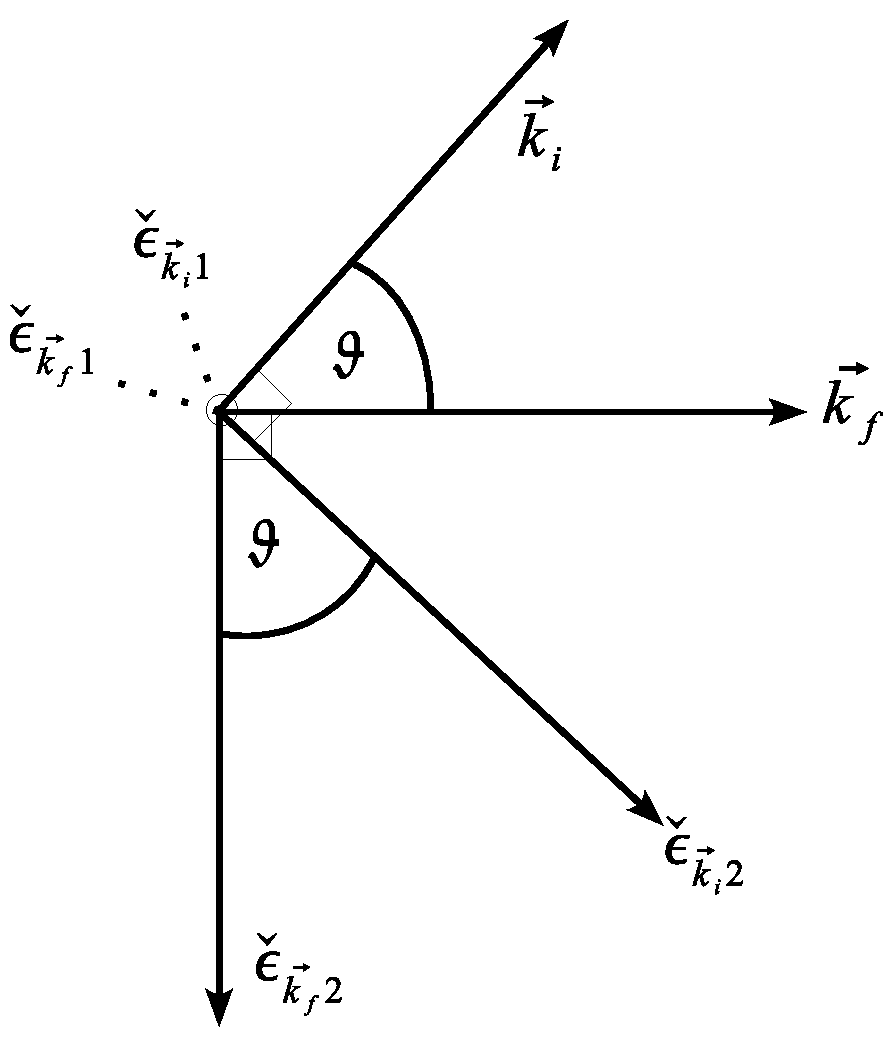
\includegraphics[height=4cm]{figs/fig-kikf.pdf}
	\caption{Geometr'ia del scattering.}
   \label{geomscat}
\end{center}
\end{figure}
\begin{eqnarray}
\frac{1}{2}\sum_{\sigma_f=1}^2\sum_{\sigma_i=1}^2\left|
\check{\varepsilon}_{\vec{k}_i\sigma_i}\cdot\check{\varepsilon}_{_{\vec
{k}_f\sigma_f}}\right|^2 & = &\frac{1}{2}\sum_{\sigma_f=1}%
^2\left\{ \left| \check{\varepsilon}_{\vec{k}_i1}\cdot\check
{\varepsilon}_{_{\vec{k}_f\sigma_f}}\right|^2+\left|
\check{\varepsilon}_{\vec{k}_i2}\cdot\check{\varepsilon}_{_{\vec{k}%
_f\sigma_f}}\right|^2\right\} \\
& = &\frac{1}{2}\left\{ \left| \check{\varepsilon}_{\vec{k}_i1}%
\cdot\check{\varepsilon}_{_{\vec{k}_f1}}\right|^2+\left|
\check{\varepsilon}_{\vec{k}_i2}\cdot\check{\varepsilon}_{_{\vec{k}_f1}%
}\right|^2\right. \nonumber\\
&&\left.+\left| \check{\varepsilon}_{\vec{k}_i1}\cdot
\check{\varepsilon}_{_{\vec{k}_f2}}\right|^2+\left|
\check{\varepsilon}_{\vec{k}_i2}\cdot\check{\varepsilon}_{_{\vec{k}_f2}%
}\right|^2\right\} \\
& = &\frac{1}{2}\left\{ 1+\cos^2\vartheta\right\} .
\end{eqnarray}


Finalmente, de estos resultados encontramos que la secci'on diferencial de
scattering de fotones con
electrones libres viene dada por:
\begin{equation}
\frac{d\sigma_{T}}{d\Omega_f}=\frac{1}{2}\left( \frac{e^2}{mc^2%
}\right)^2\left\{ 1+\cos^2\vartheta\right\}
,\label{Seccion diferencial 1}%
\end{equation}
que coincide con la secci'on transversal de scattering de Thomson.

% \subsection{Contribuci'on de segundo orden en $\hat{H}'$}
% 
% Calculemos ahora la contribuci'on a segundo orden\footnote{Esta
% contribuci'on, al igual que la dada por $\left\langle f\right| \hat
% {H}"\left| i\right\rangle  ,$ contiene t'erminos del tipo $\left\{
% \hat{a}_{\vec{k}\sigma}\hat{a}_{\vec{k}'\sigma
% '},\hat{a}_{\vec{k}\sigma}\hat{a}_{\vec{k}'\sigma
% '}^\dagger ,\hat{a}_{\vec{k}\sigma}^\dagger \hat{a}_{\vec{k}'\sigma
% '},\hat{a}_{\vec{k}\sigma}^\dagger \hat{a}_{\vec{k}'\sigma
% '}^\dagger \right\}$.} (segundo t'ermino del miembro derecho de
% (\ref{Mfi(3)})) del Hamiltoniano de interacci'on $\hat{H}'$:
% \begin{equation}
% M_{\rm fi}^{\left( 2\right) }=\sum_{I}\frac{\left\langle
%f\right|\hat{H}'\left|
% I\right\rangle  \left\langle I\right| \hat{H}'\left|
%i\right\rangle }{E_i-E_{I}}.
% \end{equation}
% 
% Nuevamente, nos preocupamos del scattering de fotones, por lo tanto los
% 'unicos t'erminos que contribuyen son
% $\hat{a}_{\vec{k}\sigma}^\dagger \hat{a}_{\vec{k}'\sigma '}$ (que producen
% procesos de \textit{absorci'on-emisi'on). }Debido a que
% en esta contribuci'on hay que considerar todos los estados intermedios para
% el electr'on libre, el diagrama del proceso es de la forma mostrada en
% la figura
% \ref{fefe}:
% \begin{figure}
% \begin{center}
% \begin{fmffile}{d4}
% \begin{fmfgraph*}(40,70)
%  \fmfbottom{ei,fi}\fmflabel{$q_i$}{ei}\fmflabel{$k_i$}{fi}
%  \fmftop{ef,ff}\fmflabel{$q_f$}{ef}\fmflabel{$k_f$}{ff}
%  \fmf{photon}{fi,v1}
%  \fmf{fermion}{ei,v1}
%  \fmf{fermion,label=$q_I$}{v1,v2}
%  \fmf{fermion}{v2,ef}
% \fmf{photon}{v2,ff}
%  %\fmfdot{v1}
%  \end{fmfgraph*}
% \end{fmffile}
% \caption{Contribuci'on a segundo orden debido a $\hat{H}'$.}
% \label{fefe}
% \end{center}
% \end{figure}
% 
% 
% Los estados inicial y final del sistema compuesto se mantienen igual al caso
% anterior (ecuaciones(\ref\label{|i>} ),(\ref{|f>} )). Denotando
% $\Theta:=\sum_{\vec{q}_{I}}\left\langle f\right| \hat{H}'\left|
% \vec{q}_{I}\right\rangle  \left\langle \vec{q}_{I}\right|\hat{H}'\left|
%i\right\rangle $,
% podemos escribir
% \begin{eqnarray}
% \Theta & = &\sum_{\vec{q}_{I}}\left\langle f\right|
% \left( -\frac{e}{mc}\sqrt{\frac{2\pi\hbar c^2}{L^3}}\sum_{\vec{k},\sigma}
%\frac{\hat{\vec{p}}\cdot\check{\varepsilon}_{\vec{k}\sigma}}{\omega
%_k^{1/2}}\left\{\hat{a}_{\vec{k}\sigma}e^{i\vec{k}\cdot\vec{x}}+\hat{a}_{\vec{k
%}\sigma}^{\dagger
% }e^{-i\vec{k}\cdot\vec{x}}\right\} \right)\left| \vec{q}_{I}\right\rangle  \\
% && \times\left\langle \vec{q}_{I}\right| \left( -\frac{e}{mc}\sqrt
% {\frac{2\pi\hbar c^2}{L^3}}\sum_{\vec{k},\sigma}\frac{\vec
% {\hat{p}}\cdot\check{\varepsilon}_{\vec{k}\sigma}}{\omega_k^{1/2}}\left\{
% \hat{a}_{\vec{k}\sigma}e^{i\vec{k}\cdot\vec{x}}+\hat{a}_{\vec{k}\sigma
% }^\dagger e^{-i\vec{k}\cdot\vec{x}}\right\} \right) \left|
% i\right\rangle  \\
% & = &\left( \frac{e}{mc}\right)^2\left( \frac{2\pi\hbar c^2}{L^3%
% }\right) \sum_{\vec{q}_{I}}\sum_{\vec{k},\sigma,\vec{k}',\sigma '}\left(
% \omega_k\omega_{k'}\right) ^{-\frac{1}{2}}\\
% && \times\left\langle \vec{q}_f\right| \left\langle \dots,n_{\vec{k}%
% _i\sigma_i}-1,\dots,n_{\vec{k}_f\sigma_f}+1,\dots\right|
% \hat{\vec{p}}\cdot\check{\varepsilon}_{\vec{k}'\sigma '}\left\{
% \hat{a}_{\vec{k}'\sigma '}e^{i\vec{k}'\cdot\vec{x}}+\hat{a}_{\vec{k}'\sigma
% '}^\dagger e^{-i\vec{k}'\cdot\vec{x}}\right\} \left| \vec{q}_{I}\right\rangle 
%\\
% && \times\left\langle \vec{q}_{I}\right| \hat{\vec{p}}%
% \cdot\check{\varepsilon}_{\vec{k}\sigma}\left\{ \hat{a}_{\vec{k}\sigma
% }e^{i\vec{k}\cdot\vec{x}}+\hat{a}_{\vec{k}\sigma}^\dagger e^{-i\vec{k}%
% \cdot\vec{x}}\right\} \left| \vec{q}_i\right\rangle  \left|
% \dots,n_{\vec{k}_i\sigma_i},\dots,n_{\vec{k}_f\sigma_f},\dots\right\rangle  \\
% & = &\left( \frac{e}{mc}\right)^2\left( \frac{2\pi\hbar c^2}{L^3%
% }\right) \sum_{\vec{q}_{I}}\sum_{\vec{k},\sigma,\vec{k}',\sigma '}\left(
% \omega_k\omega_{k'}\right) ^{-\frac{1}{2}}\\
% && \times\left\{\left\langle \gamma_f\right| \hat{a}_{\vec{k}'\sigma
% '}\hat{a}_{\vec{k}\sigma}\left| \gamma_i\right\rangle  \left\langle
% \vec{q}_f\right|
% \hat{\vec{p}}\cdot\check{\varepsilon}_{\vec{k}'\sigma
% '}e^{i\vec{k}'\cdot\vec{x}}\left| \vec{q}_{I}\right\rangle  \left\langle
%\vec{q}%
% _{I}\right| \hat{\vec{p}}\cdot\check{\varepsilon}_{\vec
% {k}\sigma}e^{i\vec{k}\cdot\vec{x}}\left| \vec{q}_i\right\rangle \right. \\
% &&+\left\langle \gamma_f\right| \hat{a}_{\vec{k}'\sigma
% '}\hat{a}_{\vec{k}\sigma}^\dagger \left| \gamma_i\right\rangle \left\langle
% \vec{q}_f\right| \hat{\vec{p}}\cdot
% \check{\varepsilon}_{\vec{k}'\sigma '}e^{i\vec{k}'\cdot\vec{x}}\left|
% \vec{q}_{I}\right\rangle  \left\langle \vec{q}%
% _{I}\right| \hat{\vec{p}}\cdot\check{\varepsilon}_{\vec
% {k}\sigma}e^{-i\vec{k}\cdot\vec{x}}\left| \vec{q}_i\right\rangle  \\
% &&+\left\langle \gamma_f\right| \hat{a}_{\vec{k}'\sigma
% '}^\dagger \hat{a}_{\vec{k}\sigma}\left| \gamma_i\right\rangle \left\langle
% \vec{q}_f\right| \hat{\vec{p}}\cdot
% \check{\varepsilon}_{\vec{k}'\sigma '}e^{-i\vec{k}'\cdot\vec{x}}\left|
% \vec{q}_{I}\right\rangle  \left\langle
% \vec{q}_{I}\right|\hat{\vec{p}}\cdot\check{\varepsilon}_{\vec{k}
% \sigma}e^{i\vec{k}\cdot\vec{x}}\left| \vec{q}_i\right\rangle  \\
% &&+\left\langle \gamma_f\right| \hat{a}_{\vec{k}'\sigma
% '}^\dagger \hat{a}_{\vec{k}\sigma}^\dagger \left| \gamma_i\right\rangle 
% \left\langle \vec{q}_f\right| \hat{\vec{p}}\cdot
% \check{\varepsilon}_{\vec{k}'\sigma '}e^{-i\vec{k}'\cdot\vec{x}}\left|
% \vec{q}_{I}\right\rangle  \left\langle \vec{q}_{I}\right|
% \hat{\vec{p}}\cdot\check{\varepsilon}_{\vec
% {k}\sigma}e^{-i\vec{k}\cdot\vec{x}}\left| \vec{q}_i\right\rangle  \\
% & = &\left( \frac{e}{mc}\right)^2\left( \frac{2\pi\hbar c^2}{L^3%
% }\right) \sum_{\vec{q}_{I}}\sum_{\vec{k},\sigma,\vec{k}',\sigma '}\left(
% \omega_k\omega_{k'}\right) ^{-\frac{1}{2}}\\
% && \times\left\{\left\langle \gamma_f\right| \hat{a}_{\vec{k}'\sigma
% '}\hat{a}_{\vec{k}\sigma}^\dagger \left| \gamma_i\right\rangle 
% \left\langle \vec{q}_f\right|
% \hat{\vec{p}}\cdot\check{\varepsilon}_{\vec{k}'\sigma
% '}e^{i\vec{k}'\cdot\vec{x}}\left| \vec{q}_{I}\right\rangle  \left\langle
%\vec{q}%
% _{I}\right| \hat{\vec{p}}\cdot\check{\varepsilon}_{\vec
% {k}\sigma}e^{-i\vec{k}\cdot\vec{x}}\left| \vec{q}_i\right\rangle  \right.\\
% &&+\left\langle \gamma_f\right| \hat{a}_{\vec{k}' \sigma
% '}^\dagger \hat{a}_{\vec{k}\sigma}\left| \gamma_i\right\rangle 
% \left\langle \vec{q}_f\right|
% \hat{\vec{p}}\cdot\check{\varepsilon}_{\vec{k}'\sigma
% '}e^{-i\vec{k}'\cdot\vec{x}}\left| \vec{q}_{I}\right\rangle  \left\langle
%\vec{q}%
% _{I}\right| \hat{\vec{p}}\cdot\check{\varepsilon}_{\vec
% {k}\sigma}e^{i\vec{k}\cdot\vec{x}}\left| \vec{q}_i\right\rangle  \\
% & = &\left( \frac{e}{mc}\right)^2\left( \frac{2\pi\hbar c^2}{L^3%
% }\right) \sum_{\vec{q}_{I}}\sum_{\vec{k},\sigma,\vec{k}',\sigma '}\left(
% \omega_k\omega_{k'}\right) ^{-\frac{1}{2}}\\
% && \times\left\{\left\langle \gamma_f\right| \hat{a}_{\vec{k}'\sigma
% '}\hat{a}_{\vec{k}\sigma}^\dagger \left| \gamma_i\right\rangle 
% \delta_{\vec{k},\vec{k}_i}\delta_{\vec{k}',\vec{k}_f}\delta_{\sigma,\sigma^{
% i}}\delta_{\sigma ',\sigma_f}\left\langle \vec{q}_f\right|
% \hat{\vec{p}}\cdot\check{\varepsilon}_{\vec{k}'\sigma
% '}e^{i\vec{k}'\cdot\vec{x}}\left| \vec{q}_{I}\right\rangle  \left\langle
% \vec{q}_{I}\right|
% \hat{\vec{p}}\cdot\check{\varepsilon}_{\vec{k}\sigma}e^{-i\vec{k}
% \cdot\vec{x}}\left| \vec{q}_i\right\rangle  \right.\\
% &&+\left\langle \gamma_f\right| \hat{a}_{\vec{k}'\sigma
% '}\hat{a}_{\vec{k}\sigma}^\dagger \left|
% \gamma_i\right\rangle \delta_{\vec{k},\vec{k}_f}\delta_{\vec{k}',\vec{k}_i}
% \delta_{\sigma,\sigma_f}\delta_{\sigma
% ',\sigma_i}\left\langle\vec{q}_f\right|\hat{\vec{p}}\cdot\check{
% \varepsilon}_{\vec{k}'\sigma '}e^{i\vec{k}'\cdot\vec{x}}\left|
% \vec{q}_{I}\right\rangle  \left\langle \vec{q}_{I}\right|
% \hat{\vec{p}}\cdot\check{\varepsilon}_{\vec{k}\sigma}e^{-i\vec{k}
% \cdot\vec{x}}\left| \vec{q}_i\right\rangle  \\
% &&+\left\langle \gamma_f\right| \hat{a}_{\vec{k}'\sigma
% '}^\dagger \hat{a}_{\vec{k}\sigma}\left|
% \gamma_i\right\rangle \delta_{\vec{k},\vec{k}_i}\delta_{\vec{k}',\vec{k}_f}
% \delta_{\sigma,\sigma_i}\delta_{\sigma ',\sigma_f}\left\langle
% \vec{q}_f\right| \hat{\vec{p}}%
% \cdot\check{\varepsilon}_{\vec{k}'\sigma '}e^{-i\vec{k}'\cdot\vec{x}}\left|
% \vec{q}_{I}\right\rangle  \left\langle \vec{q}_{I}\right|
% \hat{\vec{p}}\cdot\check{\varepsilon}_{\vec{k}\sigma}e^{i\vec{k}
% \cdot\vec{x}}\left| \vec{q}_i\right\rangle  \\
% &&+\left\langle \gamma_f\right| \hat{a}_{\vec{k}'\sigma
% '}^\dagger \hat{a}_{\vec{k}\sigma}\left|
% \gamma_i\right\rangle \delta_{\vec{k},\vec{k}_f}\delta_{\vec{k}',\vec{k}_i}
% \delta_{\sigma,\sigma_f}\delta_{\sigma ',\sigma_i}\left\langle
% \vec{q}_f\right| \hat{\vec{p}}%
% \cdot\check{\varepsilon}_{\vec{k}'\sigma '}e^{-i\vec{k}'\cdot\vec{x}}\left|
% \vec{q}_{I}\right\rangle  \left\langle \vec{q}_{I}\right|
% \hat{\vec{p}}\cdot\check{\varepsilon}_{\vec{k}\sigma}e^{i\vec{k}
% \cdot\vec{x}}\left| \vec{q}_i\right\rangle  \\
% & = &\left( \frac{e}{mc}\right)^2\left( \frac{2\pi\hbar c^2}{L^3%
% }\right) \left( \omega_{ki}\omega_{k_f}\right) ^{-\frac{1}{2}}\\
% && \times\sum_{\vec{q}_{I}}\left\{
% \left\langle \gamma_f\right| \hat{a}_{\vec{k}_f\sigma_f}\hat
% {a}_{\vec{k}_i\sigma_i}^\dagger \left| \gamma_i\right\rangle 
% \left\langle \vec{q}_f\right| \hat{\vec{p}}\cdot
% \check{\varepsilon}_{\vec{k}_f\sigma_f}e^{i\vec{k}_f\cdot\vec{x}%
% }\left| \vec{q}_{I}\right\rangle  \left\langle \vec{q}_{I}\right|
% \hat{\vec{p}}\cdot\check{\varepsilon}_{\vec{k}_i\sigma_i%
% }e^{-i\vec{k}_i\cdot\vec{x}}\left| \vec{q}_i\right\rangle  \right.\\
% &&+\left\langle \gamma_f\right| \hat{a}_{\vec{k}_i\sigma_i}\hat
% {a}_{\vec{k}_f\sigma_f}^\dagger \left| \gamma_i\right\rangle 
% \left\langle \vec{q}_f\right| \hat{\vec{p}}\cdot
% \check{\varepsilon}_{\vec{k}_i\sigma_i}e^{i\vec{k}_i\cdot\vec{x}%
% }\left| \vec{q}_{I}\right\rangle  \left\langle \vec{q}_{I}\right|
% \hat{\vec{p}}\cdot\check{\varepsilon}_{\vec{k}_f\sigma_f%
% }e^{-i\vec{k}_f\cdot\vec{x}}\left| \vec{q}_i\right\rangle  \\
% &&+\left\langle \gamma_f\right| \hat{a}_{\vec{k}_f\sigma_f}^{\dagger
% }\hat{a}_{\vec{k}_i\sigma_i}\left| \gamma_i\right\rangle 
% \left\langle \vec{q}_f\right| \hat{\vec{p}}\cdot
% \check{\varepsilon}_{\vec{k}_f\sigma_f}e^{-i\vec{k}_f\cdot\vec{x}%
% }\left| \vec{q}_{I}\right\rangle  \left\langle \vec{q}_{I}\right|
% \hat{\vec{p}}\cdot\check{\varepsilon}_{\vec{k}_i\sigma_i%
% }e^{i\vec{k}_i\cdot\vec{x}}\left| \vec{q}_i\right\rangle  \\
% &&+\left\langle \gamma_f\right| \hat{a}_{\vec{k}_i\sigma_i}^{\dagger
% }\hat{a}_{\vec{k}_f\sigma_f}\left| \gamma_i\right\rangle 
% \left\langle \vec{q}_f\right| \hat{\vec{p}}\cdot
% \check{\varepsilon}_{\vec{k}_i\sigma_i}e^{-i\vec{k}_i\cdot\vec{x}%
% }\left| \vec{q}_{I}\right\rangle  \left\langle \vec{q}_{I}\right|
% \hat{\vec{p}}\cdot\check{\varepsilon}_{\vec{k}_f\sigma_f%
% }e^{i\vec{k}_f\cdot\vec{x}}\left| \vec{q}_i\right\rangle  \\
% & = &\left( \frac{e}{mc}\right)^2\left( \frac{2\pi\hbar c^2}{L^3%
% }\right) \sqrt{\frac{n_{\vec{k}_i\sigma_i}\left( n_{\vec{k}_f%
% \sigma_f}+1\right) }{\omega_{ki}\omega_{k_f}}}\sum_{\vec{q}_{I}}\left\{
% \left\langle \vec{q}_f\right| \hat{\vec{p}}\cdot
% \check{\varepsilon}_{\vec{k}_i\sigma_i}e^{i\vec{k}_i\cdot\vec{x}%
% }\left| \vec{q}_{I}\right\rangle  \left\langle \vec{q}_{I}\right|
% \hat{\vec{p}}\cdot\check{\varepsilon}_{\vec{k}_f\sigma_f%
% }e^{-i\vec{k}_f\cdot\vec{x}}\left| \vec{q}_i\right\rangle  \right.\\
% &&+\left\langle \vec{q}_f\right| \hat{\vec{p}}\cdot
% \check{\varepsilon}_{\vec{k}_f\sigma_f}e^{-i\vec{k}_f\cdot\vec{x}%
% }\left| \vec{q}_{I}\right\rangle  \left\langle \vec{q}_{I}\right|
% \hat{\vec{p}}\cdot\check{\varepsilon}_{\vec{k}_i\sigma_i%
% }e^{i\vec{k}_i\cdot\vec{x}}\left| \vec{q}_i\right\rangle  \\
% & = &\left( \frac{e}{mc}\right)^2\left( \frac{2\pi\hbar c^2}{L^3%
% }\right) \sqrt{\frac{n_{\vec{k}_i\sigma_i}\left( n_{\vec{k}_f%
% \sigma_f}+1\right) }{\omega_{ki}\omega_{k_f}}}S\left( \vec{q}%
% _{I}\right) ,
% \end{eqnarray}
% donde hemos usado el hecho que los t'erminos del tipo $\hat{a}_{\vec{k}'\sigma
% '}\hat{a}_{\vec{k}\sigma}$ y $\hat{a}_{\vec{k}'\sigma
% '}^\dagger \hat{a}_{\vec{k}\sigma}^\dagger $ se anulan al calcular el
% correspondiente elemento $\left\langle \gamma_f\right| \left.
% {}\right. \left| \gamma_i\right\rangle  $. Analizando por separado los
%t'erminos,
% encontramos que
% \begin{eqnarray}
% \left\langle \vec{q}_f\right| \hat{\vec{p}}\cdot
% \check{\varepsilon}_{\vec{k}_i\sigma_i}e^{i\vec{k}_i\cdot\vec{x}%
% }\left| \vec{q}_{I}\right\rangle  & = &\hbar\left( \vec{q}_f\cdot
% \check{\varepsilon}_{\vec{k}_i\sigma_i}\right) \left\langle \vec{q}%
% _f\right| e^{i\vec{k}_i\cdot\vec{x}}\left| \vec{q}_{I}%
% \right\rangle  \\
% & = &\hbar\left( \vec{q}_f\cdot\check{\varepsilon}_{\vec{k}_i\sigma_i%
% }\right) \int_{L^3}\left( \frac{1}{\sqrt{L^3}}e^{-i\vec{q}_f\cdot
% \vec{x}}\right) e^{i\vec{k}_i\cdot\vec{x}}\left( \frac{1}{\sqrt{L^3}%
% }e^{i\vec{q}_{I}\cdot\vec{x}}\right) d^3x\\
% & = &\frac{\hbar}{L^3}\left( \vec{q}_f\cdot\check{\varepsilon}_{\vec
% {k}_i\sigma_i}\right) \int_{L^3}e^{i\left\{ \vec{q}_{I}-\left(
% \vec{q}_f-\vec{k}_i\right) \right\} \cdot\vec{x}}d^3x\\
% & = &\frac{\hbar}{L^3}\left( \vec{q}_f\cdot\check{\varepsilon}_{\vec
% {k}_i\sigma_i}\right) \left\{ L^3\delta_{\vec{q}_{I},\vec{q}_f%
% -\vec{k}_i}\right\} \\
% & = &\hbar\left( \vec{q}_f\cdot\check{\varepsilon}_{\vec{k}_i\sigma_i%
% }\right) \delta_{\vec{q}_{I},\vec{q}_f-\vec{k}_i},
% \end{eqnarray}
% \begin{eqnarray}
% \left\langle \vec{q}_{I}\right| \hat{\vec{p}}\cdot
% \check{\varepsilon}_{\vec{k}_f\sigma_f}e^{-i\vec{k}_f\cdot\vec{x}%
% }\left| \vec{q}_i\right\rangle  & = &\hbar\left( \vec{q}_{I}\cdot
% \check{\varepsilon}_{\vec{k}_f\sigma_f}\right) \left\langle \vec{q}%
% _{I}\right| e^{-i\vec{k}_f\cdot\vec{x}}\left| \vec{q}_i%
% \right\rangle  \\
% & = &\hbar\left( \vec{q}_{I}\cdot\check{\varepsilon}_{\vec{k}_f\sigma_f%
% }\right) \int_{L^3}\left( \frac{1}{\sqrt{L^3}}e^{-i\vec{q}_{I}\cdot
% \vec{x}}\right) e^{-i\vec{k}_f\cdot\vec{x}}\left( \frac{1}{\sqrt{L^3}%
% }e^{i\vec{q}_i\cdot\vec{x}}\right) d^3x\\
% & = &\frac{\hbar}{L^3}\left( \vec{q}_{I}\cdot\check{\varepsilon}_{\vec
% {k}_f\sigma_f}\right) \int_{L^3}e^{-i\left\{ \vec{q}_{I}-\left(
% \vec{q}_i-\vec{k}_f\right) \right\} \cdot\vec{x}}d^3x\\
% & = &\frac{\hbar}{L^3}\left( \vec{q}_{I}\cdot\check{\varepsilon}_{\vec
% {k}_f\sigma_f}\right) \left\{ L^3\delta_{\vec{q}_{I},\vec{q}_i%
% -\vec{k}_f}\right\} \\
% & = &\hbar\left( \vec{q}_{I}\cdot\check{\varepsilon}_{\vec{k}_f\sigma_f%
% }\right) \delta_{\vec{q}_{I},\vec{q}_i-\vec{k}_f},
% \end{eqnarray}
% \begin{eqnarray}
% \left\langle \vec{q}_f\right| \hat{\vec{p}}\cdot
% \check{\varepsilon}_{\vec{k}_f\sigma_f}e^{-i\vec{k}_f\cdot\vec{x}%
% }\left| \vec{q}_{I}\right\rangle  & = &\hbar\left( \vec{q}_f\cdot
% \check{\varepsilon}_{\vec{k}_f\sigma_f}\right) \left\langle \vec{q}%
% _f\right| e^{-i\vec{k}_f\cdot\vec{x}}\left| \vec{q}_{I}%
% \right\rangle  \\
% & = &\hbar\left( \vec{q}_f\cdot\check{\varepsilon}_{\vec{k}_f\sigma_f%
% }\right) \int_{L^3}\left( \frac{1}{\sqrt{L^3}}e^{-i\vec{q}_f\cdot
% \vec{x}}\right) e^{-i\vec{k}_f\cdot\vec{x}}\left( \frac{1}{\sqrt{L^3}%
% }e^{i\vec{q}_{I}\cdot\vec{x}}\right) d^3x\\
% & = &\frac{\hbar}{L^3}\left( \vec{q}_f\cdot\check{\varepsilon}_{\vec
% {k}_f\sigma_f}\right) \int_{L^3}e^{i\left\{ \vec{q}_{I}-\left(
% \vec{q}_f+\vec{k}_f\right) \right\} \cdot\vec{x}}d^3x\\
% & = &\frac{\hbar}{L^3}\left( \vec{q}_f\cdot\check{\varepsilon}_{\vec
% {k}_f\sigma_f}\right) \left\{ L^3\delta_{\vec{q}_{I},\vec{q}_f%
% +\vec{k}_f}\right\} \\
% & = &\hbar\left( \vec{q}_f\cdot\check{\varepsilon}_{\vec{k}_f\sigma_f%
% }\right) \delta_{\vec{q}_{I},\vec{q}_f+\vec{k}_f},
% \end{eqnarray}
% \begin{eqnarray}
% \left\langle \vec{q}_{I}\right| \hat{\vec{p}}\cdot
% \check{\varepsilon}_{\vec{k}_i\sigma_i}e^{i\vec{k}_i\cdot\vec{x}%
% }\left| \vec{q}_i\right\rangle  & = &\hbar\left( \vec{q}_{I}\cdot
% \check{\varepsilon}_{\vec{k}_i\sigma_i}\right) \left\langle \vec{q}%
% _{I}\right| e^{i\vec{k}_i\cdot\vec{x}}\left| \vec{q}_i%
% \right\rangle  \\
% & = &\hbar\left( \vec{q}_{I}\cdot\check{\varepsilon}_{\vec{k}_i\sigma_i%
% }\right) \int_{L^3}\left( \frac{1}{\sqrt{L^3}}e^{-i\vec{q}_{I}\cdot
% \vec{x}}\right) e^{i\vec{k}_i\cdot\vec{x}}\left( \frac{1}{\sqrt{L^3}%
% }e^{i\vec{q}_i\cdot\vec{x}}\right) d^3x\\
% & = &\frac{\hbar}{L^3}\left( \vec{q}_{I}\cdot\check{\varepsilon}_{\vec
% {k}_i\sigma_i}\right) \int_{L^3}e^{-i\left\{ \vec{q}_{I}-\left(
% \vec{k}_i+\vec{q}_i\right) \right\} \cdot\vec{x}}d^3x\\
% & = &\frac{\hbar}{L^3}\left( \vec{q}_{I}\cdot\check{\varepsilon}_{\vec
% {k}_i\sigma_i}\right) \left\{ L^3\delta_{\vec{q}_{I},\vec{k}_i%
% +\vec{q}_i}\right\} \\
% & = &\hbar\left( \vec{q}_{I}\cdot\check{\varepsilon}_{\vec{k}_i\sigma_i%
% }\right) \delta_{\vec{q}_{I},\vec{k}_i+\vec{q}_i}.
% \end{eqnarray}
% Luego:
% \begin{eqnarray}
% S\left( \vec{q}_{I}\right) & = &\sum_{\vec{q}_{I}}\left\{ \left[
% \hbar\left( \vec{q}_f\cdot\check{\varepsilon}_{\vec{k}_i\sigma_i%
% }\right) \delta_{\vec{q}_{I},\vec{q}_f-\vec{k}_i}\right] \left[
% \hbar\left( \vec{q}_{I}\cdot\check{\varepsilon}_{\vec{k}_f\sigma_f%
% }\right) \delta_{\vec{q}_{I},\vec{q}_i-\vec{k}_f}\right] +\left[
% \hbar\left( \vec{q}_f\cdot\check{\varepsilon}_{\vec{k}_f\sigma_f%
% }\right) \delta_{\vec{q}_{I},\vec{q}_f+\vec{k}_f}\right] \left[
% \hbar\left( \vec{q}_{I}\cdot\check{\varepsilon}_{\vec{k}_i\sigma_i%
% }\right) \delta_{\vec{q}_{I},\vec{k}_i+\vec{q}_i}\right] \right\} \\
% & = &\sum_{\vec{q}_{I}}\left\{ \hbar^2\left( \vec{q}_f\cdot
% \check{\varepsilon}_{\vec{k}_i\sigma_i}\right) \left( \vec{q}_{I}%
% \cdot\check{\varepsilon}_{\vec{k}_f\sigma_f}\right) \delta_{\vec{q}%
% _{I},\vec{q}_f-\vec{k}_i}\delta_{\vec{q}_{I},\vec{q}_i-\vec{k}_f%
% }+\hbar^2\left( \vec{q}_f\cdot\check{\varepsilon}_{\vec{k}_f\sigma_f%
% }\right) \left( \vec{q}_{I}\cdot\check{\varepsilon}_{\vec{k}_i\sigma_i%
% }\right) \delta_{\vec{q}_{I},\vec{q}_f+\vec{k}_f}\delta_{\vec{q}_{I}%
% ,\vec{k}_i+\vec{q}_i}\right\} .
% \end{eqnarray}
% 
% 
% As'i, el elemento de matriz buscado es:%
% \begin{eqnarray}
% \sum_{I}\frac{\left\langle f\right| \hat{H}'\left|
% I\right\rangle  \left\langle I\right| \hat{H}'\left|
% i\right\rangle  }{E_i-E_{I}} & = &\left( \frac{e}{mc}\right)^2\left(
% \frac{2\pi\hbar c^2}{L^3}\right) \sqrt{\frac{n_{\vec{k}_i\sigma_i%
% }\left( n_{\vec{k}_f\sigma_f}+1\right) }{\omega_{ki}\omega_{k_f}}%
% }\nonumber\\
% && \times\sum_{\vec{q}_{I}}\left\{\frac{\hbar^2\left(
% \vec{q}_f\cdot\check{\varepsilon}_{\vec{k}_i%
% \sigma_i}\right) \left( \vec{q}_{I}\cdot\check{\varepsilon}_{\vec{k}%
% _f\sigma_f}\right) }{\left( \frac{\hbar^2}{2m}\vec{q}_i^2%
% +\hbar\omega_{k_i}n_{\vec{k}_i\sigma_i}\right) -\left( \frac{\hbar
%^2}{2m}\vec{q}_{I}^2+\hbar\omega_{k_i}n_{\vec{k}_i\sigma_i}%
% -\hbar\omega_{k_i}\right) }\delta_{\vec{q}_{I},\vec{q}_f-\vec{k}_i%
% }\delta_{\vec{q}_{I},\vec{q}_i-\vec{k}_f}\right.\\
% &&\left.+\frac{\hbar^2\left( \vec{q}_f\cdot\check{\varepsilon}_{\vec{k}_f%
% \sigma_f}\right) \left( \vec{q}_{I}\cdot\check{\varepsilon}_{\vec{k}%
% _i\sigma_i}\right) }{\left( \frac{\hbar^2}{2m}\vec{q}_i^2%
% +\hbar\omega_{k_i}n_{\vec{k}_i\sigma_i}\right) -\left( \frac{\hbar
%^2}{2m}\vec{q}_{I}^2+\hbar\omega_{k_i}n_{\vec{k}_i\sigma_i}%
% -\hbar\omega_{k_i}\right) }\delta_{\vec{q}_{I},\vec{q}_f+\vec{k}_f%
% }\delta_{\vec{q}_{I},\vec{k}_i+\vec{q}_i} \right.\nonumber\\
% & = &\left( \frac{e}{mc}\right)^2\left( \frac{2\pi\hbar c^2}{L^3%
% }\right) \sqrt{\frac{n_{\vec{k}_i\sigma_i}\left( n_{\vec{k}_f%
% \sigma_f}+1\right) }{\omega_{ki}\omega_{k_f}}}\nonumber\\
% && \times\sum_{\vec{q}_{I}}\left\{
% \frac{\hbar^2\left( \vec{q}_f\cdot\check{\varepsilon}_{\vec{k}_i%
% \sigma_i}\right) \left( \vec{q}_{I}\cdot\check{\varepsilon}_{\vec{k}%
% _f\sigma_f}\right) }{\frac{\hbar^2}{2m}\left( \vec{q}_i^2-\vec
% {q}_{I}^2\right) +\hbar\omega_{k_i}}\delta_{\vec{q}_{I},\vec{q}_f%
% -\vec{k}_i}\delta_{\vec{q}_{I},\vec{q}_i-\vec{k}_f}\right.\\
% &&+\frac{\hbar^2\left( \vec{q}_f\cdot\check{\varepsilon}_{\vec{k}_f%
% \sigma_f}\right) \left( \vec{q}_{I}\cdot\check{\varepsilon}_{\vec{k}%
% _i\sigma_i}\right) }{\frac{\hbar^2}{2m}\left( \vec{q}_i^2-\vec
% {q}_{I}^2\right) +\hbar\omega_{k_i}}\delta_{\vec{q}_{I},\vec{q}_f%
% +\vec{k}_f}\delta_{\vec{q}_{I},\vec{k}_i+\vec{q}_i}%
%  \nonumber\\
% & = &\left( \frac{e}{mc}\right)^2\left( \frac{2\pi\hbar c^2}{L^3%
% }\right) \sqrt{\frac{n_{\vec{k}_i\sigma_i}\left( n_{\vec{k}_f%
% \sigma_f}+1\right) }{\omega_{ki}\omega_{k_f}}}\nonumber\\
% && \times\left\{
% \frac{\hbar^2\left( \vec{q}_f\cdot\check{\varepsilon}_{\vec{k}_i%
% \sigma_i}\right) \left( \left( \vec{q}_i-\vec{k}_f\right)
% \cdot\check{\varepsilon}_{\vec{k}_f\sigma_f}\right)
% }{\frac{\hbar^2}{2m}\left( \vec{q}_i^2-\left(
% \vec{q}_i-\vec{k}_f\right)
%^2\right) +\hbar\omega_{k_i}}\delta_{\vec{q}_i-\vec{k}_f,\vec{q}%
% _f-\vec{k}_i}\right.\\
% &&+\frac{\hbar^2\left( \vec{q}_f\cdot\check{\varepsilon}_{\vec{k}_f%
% \sigma_f}\right) \left( \left( \vec{k}_i+\vec{q}_i\right)
% \cdot\check{\varepsilon}_{\vec{k}_i\sigma_i}\right)
% }{\frac{\hbar^2}{2m}\left( \vec{q}_i^2-\left(
% \vec{k}_i+\vec{q}_i\right)^2\right)
% +\hbar\omega_{k_i}}\delta_{\vec{k}_i+\vec{q}_i,\vec{q}%
% _f+\vec{k}_f}
% \nonumber\\
% & = &2\left( \frac{e^2}{2mc^2}\right) \left( \frac{2\pi\hbar c^2%
% }{L^3}\right) \sqrt{\frac{n_{\vec{k}_i\sigma_i}\left( n_{\vec{k}%
% _f\sigma_f}+1\right) }{\omega_{ki}\omega_{k_f}}}\delta_{\vec{k}%
% _i+\vec{q}_i,\vec{q}_f+\vec{k}_f}\nonumber\\
% && \times\left\{ \frac{\frac{\hbar^2}{m}\left( \vec{q}_f\cdot
% \check{\varepsilon}_{\vec{k}_i\sigma_i}\right) \left( \vec{q}_i%
% \cdot\check{\varepsilon}_{\vec{k}_f\sigma_f}-\vec{k}_f\cdot
% \check{\varepsilon}_{\vec{k}_f\sigma_f}\right) }{\frac{\hbar^2}%
% {2m}\left( 2\vec{q}_i\cdot\vec{k}_f+\vec{k}_f^2\right) +\hbar
% \omega_{k_i}}+\frac{\frac{\hbar^2}{m}\left( \vec{q}_f\cdot
% \check{\varepsilon}_{\vec{k}_f\sigma_f}\right) \left( \vec{k}_i%
% \cdot\check{\varepsilon}_{\vec{k}_i\sigma_i}+\vec{q}_i\cdot
% \check{\varepsilon}_{\vec{k}_i\sigma_i}\right) }{\hbar\omega_{k_i%
% }-\frac{\hbar^2}{2m}\left( 2\vec{k}_i\cdot\vec{q}_i+\vec{k}_i%
%^2\right) }\right\} ,\label{Sum<f|H1|I><I|H1|i\rangle /deltaE}%
% \end{eqnarray}
% pero sabemos que%
% \begin{eqnarray}
% \vec{k}_i\cdot\check{\varepsilon}_{\vec{k}_i\sigma_i} & = &0,\\
% \vec{k}_f\cdot\check{\varepsilon}_{\vec{k}_f\sigma_f} & = &0,
% \end{eqnarray}
% ya que las ondas que describen al fot'on son transversales. Entonces, vamos a
% tener que:%
% \begin{eqnarray}
% \left| M_{\rm fi}^{\left( 2\right) }\right|^2 & = &\left|
% \sum_{I}\frac{\left\langle f\right| \hat{H}'\left|
% I\right\rangle  \left\langle I\right| \hat{H}'\left|
% i\right\rangle  }{E_i-E_{I}}\right|^2\\
% & = &4\left( \frac{e^2}{2mc^2}\right)^2\left( \frac{2\pi\hbar c^2%
% }{L^3}\right)^2\frac{n_{\vec{k}_i\sigma_i}\left( n_{\vec{k}%
% _f\sigma_f}+1\right) }{\omega_{ki}\omega_{k_f}}\\
% && \times\left| \frac{\frac{\hbar^2}{m}\left( \vec{q}_f\cdot
% \check{\varepsilon}_{\vec{k}_i\sigma_i}\right) \left( \vec{q}_i%
% \cdot\check{\varepsilon}_{\vec{k}_f\sigma_f}\right) }{\frac{\hbar^2%
% }{2m}\left( 2\vec{q}_i\cdot\vec{k}_f+\vec{k}_f^2\right) +\hbar
% \omega_{k_i}}+\frac{\frac{\hbar^2}{m}\left( \vec{q}_f\cdot
% \check{\varepsilon}_{\vec{k}_f\sigma_f}\right) \left( \vec{q}_i%
% \cdot\check{\varepsilon}_{\vec{k}_i\sigma_i}\right) }{\hbar\omega_{k_i%
% }-\frac{\hbar^2}{2m}\left( 2\vec{k}_i\cdot\vec{q}_i+\vec{k}_i%
%^2\right) }\right|^2\delta_{\vec{k}_i+\vec{q}_i,\vec{q}_f%
% +\vec{k}_f},
% \end{eqnarray}
% y as'i, la probabilidad por unidad de tiempo de que los fotones incidentes
% sean dispersados por el electr'on es:%
% \begin{eqnarray}
% \left( \frac{P}{t}\right) _{%
% \genfrac{.}{.}{0pt}{}{Photon}{Scattering}%
% } & = &\frac{2\pi}{\hbar}\left| M_{\rm fi}\right|^2\delta\left(
% E_f-E_i\right) \\
% & = &\frac{8\pi}{\hbar}\left( \frac{e^2}{2mc^2}\right)^2\left(
% \frac{2\pi\hbar c^2}{L^3}\right)^2\frac{n_{\vec{k}_i\sigma_i%
% }\left( n_{\vec{k}_f\sigma_f}+1\right) }{\omega_{ki}\omega_{k_f}}\\
% && \times\left| \frac{\frac{\hbar^2}{m}\left( \vec{q}_f\cdot
% \check{\varepsilon}_{\vec{k}_i\sigma_i}\right) \left( \vec{q}_i%
% \cdot\check{\varepsilon}_{\vec{k}_f\sigma_f}\right) }{\frac{\hbar^2%
% }{2m}\left( 2\vec{q}_i\cdot\vec{k}_f+\vec{k}_f^2\right) +\hbar
% \omega_{k_i}}+\frac{\frac{\hbar^2}{m}\left( \vec{q}_f\cdot
% \check{\varepsilon}_{\vec{k}_f\sigma_f}\right) \left( \vec{q}_i%
% \cdot\check{\varepsilon}_{\vec{k}_i\sigma_i}\right) }{\hbar\omega_{k_i%
% }-\frac{\hbar^2}{2m}\left( 2\vec{k}_i\cdot\vec{q}_i+\vec{k}_i%
%^2\right) }\right|^2\\
% && \times\delta_{\vec{k}_i+\vec{q}_i,\vec{q}_f+\vec{k}_f}\delta\left(
% \frac{\left( \hbar\vec{q}_f\right)^2}{2m}+\hbar\omega_{k_f}%
% -\frac{\left( \hbar\vec{q}_i\right)^2}{2m}-\hbar\omega_{k_i}\right)
% .
% \end{eqnarray}
% 
% 
% Reemplazando la expresi'on anterior en (\ref{Seccion Transversal Absorcion}%
% ), y haciendo nuevamente\footnote{Ya que como vimos, el t'ermino $\left(
% n_{\vec{k}_f\sigma_f}+1\right) $ es interpretado como emisi'on
% estimulada por los fotones $\vec{k}_f\sigma_f$ en el estado final.}
% $n_{\vec{k}_f\sigma_f}=0$, tendremos:%
% \begin{eqnarray}
% \sigma\left( \vec{k}\sigma\right) & = &\frac{\left( \frac{P}{t}\right) _{%
% \genfrac{.}{.}{0pt}{}{Photon}{Scattering}}}{\frac{n_{\vec{k}_i\sigma_i}}{L^{
% 3}}c}\nonumber\\
% & = &\frac{8\pi L^3}{\hbar c}\left( \frac{e^2}{2mc^2}\right)
%^2\left( \frac{2\pi\hbar c^2}{L^3}\right)^2\frac{1}{\omega
% _{ki}\omega_{k_f}}\nonumber\\
% && \times\left| \frac{\frac{\hbar^2}{m}\left( \vec{q}_f\cdot
% \check{\varepsilon}_{\vec{k}_i\sigma_i}\right) \left( \vec{q}_i%
% \cdot\check{\varepsilon}_{\vec{k}_f\sigma_f}\right) }{\frac{\hbar^2%
% }{2m}\left( 2\vec{q}_i\cdot\vec{k}_f+\vec{k}_f^2\right) +\hbar
% \omega_{k_i}}+\frac{\frac{\hbar^2}{m}\left( \vec{q}_f\cdot
% \check{\varepsilon}_{\vec{k}_f\sigma_f}\right) \left( \vec{q}_i%
% \cdot\check{\varepsilon}_{\vec{k}_i\sigma_i}\right) }{\hbar\omega_{k_i%
% }-\frac{\hbar^2}{2m}\left( 2\vec{k}_i\cdot\vec{q}_i+\vec{k}_i%
%^2\right) }\right|^2\nonumber\\
% && \times\delta_{\vec{k}_i+\vec{q}_i,\vec{q}_f+\vec{k}_f}\delta\left(
% \frac{\left( \hbar\vec{q}_f\right)^2}{2m}+\hbar\omega_{k_f}%
% -\frac{\left( \hbar\vec{q}_i\right)^2}{2m}-\hbar\omega_{k_i}\right)
% .\label{Seccion Transversal Absorcion <f|H1|I><I|H1|i\rangle }%
% \end{eqnarray}
% 
% 
% Las leyes de conservaci'on resultan ser las mismas que el caso anterior,
% tal cu'al se esperaba ya que los estados iniciales y finales son los mismos
% para ambos casos.
% 
% De (\ref{<f|H2|i>} ) y (\ref{Sum<f|H1|I><I|H1|i\rangle /deltaE}) tenemos
% entonces que la matriz de transici'on ser'a:%
% \begin{eqnarray}
% \left| M_{\rm fi}\right|^2 & = &\left| \left\langle f\right|
% \hat{H}''\left| i\right\rangle  +\sum_{I}\frac{\left\langle
% f\right| \hat{H}'\left| I\right\rangle  \left\langle
% I\right| \hat{H}'\left| i\right\rangle  }{E_i-E_{I}%
% }\right|^2\\
% & = &4\left( \frac{e^2}{2mc^2}\right)^2\left( \frac{2\pi\hbar c^2%
% }{L^3}\right)^2\frac{n_{\vec{k}_i\sigma_i}}{\omega_{k_i}%
% \omega_{k_f}}\left|
% \begin{array}
% [c]{c}%
% \left( \check{\varepsilon}_{\vec{k}_i\sigma_i}\cdot\check{\varepsilon
% }_{_{\vec{k}_f\sigma_f}}\right) +\frac{\frac{\hbar^2}{m}\left( \vec
% {q}_f\cdot\check{\varepsilon}_{\vec{k}_i\sigma_i}\right) \left(
% \vec{q}_i\cdot\check{\varepsilon}_{\vec{k}_f\sigma_f}-\vec{k}_f%
% \cdot\check{\varepsilon}_{\vec{k}_f\sigma_f}\right) }{\frac{\hbar^2%
% }{2m}\left( 2\vec{q}_i\cdot\vec{k}_f+\vec{k}_f^2\right) +\hbar
% \omega_{k_i}}\\
% +\frac{\frac{\hbar^2}{m}\left( \vec{q}_f\cdot\check{\varepsilon}_{\vec
% {k}_f\sigma_f}\right) \left( \vec{k}_i\cdot\check{\varepsilon}%
% _{\vec{k}_i\sigma_i}+\vec{q}_i\cdot\check{\varepsilon}_{\vec{k}%
% _i\sigma_i}\right) }{\hbar\omega_{k_i}-\frac{\hbar^2}{2m}\left(
% 2\vec{k}_i\cdot\vec{q}_i+\vec{k}_i^2\right) }%
% \end{array}
% \right|^2\delta_{\vec{q}_f+\vec{k}_f,\vec{q}_i+\vec{k}_i}.
% \end{eqnarray}
% 
% 
% Por lo tanto la secci'on transversal de absorci'on para los dos
% t'erminos considerados en la expansi'on perturbativa queda como:%
% \begin{eqnarray}
% \sigma\left( \vec{k}\sigma\right) & = &\frac{2\pi L^3}{\hbar cn_{\vec
% {k}_i\sigma_i}}\left| M_{\rm fi}\right|^2\delta\left( E_f%
% -E_i\right) \\
% & = &\frac{8\pi L^3}{\hbar c\omega_{k_i}\omega_{k_f}}\left( \frac{e^2%
% }{2mc^2}\right)^2\left( \frac{2\pi\hbar c^2}{L^3}\right)
%^2\left|
% \begin{array}
% [c]{c}%
% \left( \check{\varepsilon}_{\vec{k}_i\sigma_i}\cdot\check{\varepsilon
% }_{_{\vec{k}_f\sigma_f}}\right) +\frac{\frac{\hbar^2}{m}\left( \vec
% {q}_f\cdot\check{\varepsilon}_{\vec{k}_i\sigma_i}\right) \left(
% \vec{q}_i\cdot\check{\varepsilon}_{\vec{k}_f\sigma_f}-\vec{k}_f%
% \cdot\check{\varepsilon}_{\vec{k}_f\sigma_f}\right) }{\frac{\hbar^2%
% }{2m}\left( 2\vec{q}_i\cdot\vec{k}_f+\vec{k}_f^2\right) +\hbar
% \omega_{k_i}}\\
% +\frac{\frac{\hbar^2}{m}\left( \vec{q}_f\cdot\check{\varepsilon}_{\vec
% {k}_f\sigma_f}\right) \left( \vec{k}_i\cdot\check{\varepsilon}%
% _{\vec{k}_i\sigma_i}+\vec{q}_i\cdot\check{\varepsilon}_{\vec{k}%
% _i\sigma_i}\right) }{\hbar\omega_{k_i}-\frac{\hbar^2}{2m}\left(
% 2\vec{k}_i\cdot\vec{q}_i+\vec{k}_i^2\right) }%
% \end{array}
% \right|^2\\
% && \times\delta_{\vec{q}_f+\vec{k}_f,\vec{q}_i+\vec{k}_i}\delta\left(
% \frac{\left( \hbar\vec{q}_f\right)^2}{2m}+\hbar\omega_{k_f}%
% -\frac{\left( \hbar\vec{q}_i\right)^2}{2m}-\hbar\omega_{k_i}\right)
% ,
% \end{eqnarray}
% y si sumamos sobre todos los estados finales del fot'on y del electr'on,
% tendremos la secci'on transversal de scattering total de absorci'on del
% fot'on:%
% \begin{eqnarray}
% \sigma_{T} & = &\sum_{\vec{k}_f}\sum_{\sigma_f=1}^2\sum_{\vec{q}_f%
% }\sigma\left( \vec{k}\sigma\right) \\
% & = &\frac{8\pi L^3}{\hbar c}\left( \frac{e^2}{2mc^2}\right)
%^2\left( \frac{2\pi\hbar c^2}{L^3}\right)^2\sum_{\vec{k}_f}%
% \sum_{\sigma_f=1}^2\sum_{\vec{q}_f}\frac{\delta_{\vec{k}_i+\vec{q}%
% _i,\vec{q}_f+\vec{k}_f}}{\omega_{k_i}\omega_{k_f}}\delta\left(
% \frac{\left( \hbar\vec{q}_f\right)^2}{2m}+\hbar\omega_{k_f}%
% -\frac{\left( \hbar\vec{q}_i\right)^2}{2m}-\hbar\omega_{k_i}\right)
% \\
% && \times\left| \left( \check{\varepsilon}_{\vec{k}_i\sigma_i}%
% \cdot\check{\varepsilon}_{_{\vec{k}_f\sigma_f}}\right) +\frac{\frac
% {\hbar^2}{m}\left( \vec{q}_f\cdot\check{\varepsilon}_{\vec{k}_i%
% \sigma_i}\right) \left( \vec{q}_i\cdot\check{\varepsilon}_{\vec{k}%
% _f\sigma_f}\right) }{\frac{\hbar^2}{2m}\left( 2\vec{q}_i\cdot\vec
% {k}_f+\vec{k}_f^2\right) +\hbar\omega_{k_i}}+\frac{\frac{\hbar^2%
% }{m}\left( \vec{q}_f\cdot\check{\varepsilon}_{\vec{k}_f\sigma_f%
% }\right) \left( \vec{q}_i\cdot\check{\varepsilon}_{\vec{k}_i\sigma_i%
% }\right) }{\hbar\omega_{k_i}-\frac{\hbar^2}{2m}\left( 2\vec{k}_i%
% \cdot\vec{q}_i+\vec{k}_i^2\right) }\right|^2\\
% & = &\frac{8\pi L^3}{\hbar c}\left( \frac{e^2}{2mc^2}\right)
%^2\left( \frac{2\pi\hbar c^2}{L^3}\right)^2\sum_{\vec{k}_f}%
% \sum_{\sigma_f=1}^2\frac{\delta\left( \frac{\hbar^2\left( \vec{k}%
% _i+\vec{q}_i-\vec{k}_f\right)^2}{2m}+\hbar\omega_{k_f}%
% -\frac{\left( \hbar\vec{q}_i\right)^2}{2m}-\hbar\omega_{k_i}\right)
% }{\omega_{k_i}\omega_{k_f}}\\
% && \times\left| \left( \check{\varepsilon}_{\vec{k}_i\sigma_i}%
% \cdot\check{\varepsilon}_{_{\vec{k}_f\sigma_f}}\right) +\frac{\frac
% {\hbar^2}{m}\left( \left( \vec{k}_i+\vec{q}_i-\vec{k}_f\right)
% \cdot\check{\varepsilon}_{\vec{k}_i\sigma_i}\right) \left( \vec{q}%
% _i\cdot\check{\varepsilon}_{\vec{k}_f\sigma_f}\right) }{\frac{\hbar
%^2}{2m}\left( 2\vec{q}_i\cdot\vec{k}_f+\vec{k}_f^2\right)
% +\hbar\omega_{k_i}}+\frac{\frac{\hbar^2}{m}\left( \left( \vec{k}%
% _i+\vec{q}_i-\vec{k}_f\right) \cdot\check{\varepsilon}_{\vec{k}%
% _f\sigma_f}\right) \left( \vec{q}_i\cdot\check{\varepsilon}_{\vec
% {k}_i\sigma_i}\right) }{\hbar\omega_{k_i}-\frac{\hbar^2}{2m}\left(
% 2\vec{k}_i\cdot\vec{q}_i+\vec{k}_i^2\right) }\right|^2\\
% & = &\frac{8\pi L^3}{\hbar c}\left( \frac{e^2}{2mc^2}\right)
%^2\left( \frac{2\pi\hbar c^2}{L^3}\right)^2\sum_{\vec{k}_f}%
% \sum_{\sigma_f=1}^2\frac{\delta\left( \frac{2\hbar^2\vec{q}_i%
% \cdot\left( \vec{k}_i-\vec{k}_f\right) }{2m}+\frac{\hbar^2\left(
% \vec{k}_i-\vec{k}_f\right)^2}{2m}+\hbar\omega_{k_f}-\hbar
% \omega_{k_i}\right) }{\omega_{k_i}\omega_{k_f}}\\
% && \times\left| \left( \check{\varepsilon}_{\vec{k}_i\sigma_i}%
% \cdot\check{\varepsilon}_{_{\vec{k}_f\sigma_f}}\right) +\frac{\frac
% {\hbar^2}{m}\left( \vec{q}_i\cdot\check{\varepsilon}_{\vec{k}_i%
% \sigma_i}-\vec{k}_f\cdot\check{\varepsilon}_{\vec{k}_i\sigma_i%
% }\right) \left( \vec{q}_i\cdot\check{\varepsilon}_{\vec{k}_f\sigma_f%
% }\right) }{\frac{\hbar^2}{2m}\left( 2\vec{q}_i\cdot\vec{k}_f+\vec
% {k}_f^2\right) +\hbar\omega_{k_i}}+\frac{\frac{\hbar^2}{m}\left(
% \vec{k}_i\cdot\check{\varepsilon}_{\vec{k}_f\sigma_f}+\vec{q}_i%
% \cdot\check{\varepsilon}_{\vec{k}_f\sigma_f}\right) \left( \vec{q}%
% _i\cdot\check{\varepsilon}_{\vec{k}_i\sigma_i}\right) }{\hbar
% \omega_{k_i}-\frac{\hbar^2}{2m}\left( 2\vec{k}_i\cdot\vec{q}_i%
% +\vec{k}_i^2\right) }\right|^2.
% \end{eqnarray}
% 
% 
% Haciendo paso al continuo (y luego escribir en coordenadas esf'ericas:
% $d^3k_f=k_f^2dk_fd\Omega_{k_f}$) obtenemos:%
% \begin{eqnarray}
% \sigma_{T} & = &\frac{8\pi L^3}{\hbar c}\left( \frac{e^2}{2mc^2%
% }\right)^2\left( \frac{2\pi\hbar c^2}{L^3}\right)^2\sum
% _{\sigma_f=1}^2\left( \frac{L^3}{\left( 2\pi\right) ^3}\int_{L^3%
% }d^3k_f\right) \frac{\delta\left( \frac{2\hbar^2\vec{q}_i%
% \cdot\left( \vec{k}_i-\vec{k}_f\right) }{2m}+\frac{\hbar^2\left(
% \vec{k}_i-\vec{k}_f\right)^2}{2m}+\hbar\omega_{k_f}-\hbar
% \omega_{k_i}\right) }{\omega_{k_i}\omega_{k_f}}\\
% && \times\left| \left( \check{\varepsilon}_{\vec{k}_i\sigma_i}%
% \cdot\check{\varepsilon}_{_{\vec{k}_f\sigma_f}}\right) +\frac{\frac
% {\hbar^2}{m}\left( \vec{q}_i\cdot\check{\varepsilon}_{\vec{k}_i%
% \sigma_i}-\vec{k}_f\cdot\check{\varepsilon}_{\vec{k}_i\sigma_i%
% }\right) \left( \vec{q}_i\cdot\check{\varepsilon}_{\vec{k}_f\sigma_f%
% }\right) }{\frac{\hbar^2}{2m}\left( 2\vec{q}_i\cdot\vec{k}_f+\vec
% {k}_f^2\right) +\hbar\omega_{k_i}}+\frac{\frac{\hbar^2}{m}\left(
% \vec{k}_i\cdot\check{\varepsilon}_{\vec{k}_f\sigma_f}+\vec{q}_i%
% \cdot\check{\varepsilon}_{\vec{k}_f\sigma_f}\right) \left( \vec{q}%
% _i\cdot\check{\varepsilon}_{\vec{k}_i\sigma_i}\right) }{\hbar
% \omega_{k_i}-\frac{\hbar^2}{2m}\left( 2\vec{k}_i\cdot\vec{q}_i%
% +\vec{k}_i^2\right) }\right|^2\\
% & = &\frac{\hbar e^{4}}{m^2c}\sum_{\sigma_f=1}^2\int dk_fd\Omega
% _f\frac{k_f^2}{\omega_{k_i}\omega_{k_f}}\delta\left( \frac
% {2\hbar^2\vec{q}_i\cdot\left( \vec{k}_i-\vec{k}_f\right) }{2m}%
% +\frac{\hbar^2\left( \vec{k}_i-\vec{k}_f\right)^2}{2m}+\hbar
% \omega_{k_f}-\hbar\omega_{k_i}\right) \\
% && \times\left| \left( \check{\varepsilon}_{\vec{k}_i\sigma_i}%
% \cdot\check{\varepsilon}_{_{\vec{k}_f\sigma_f}}\right) +\frac{\frac
% {\hbar^2}{m}\left( \vec{q}_i\cdot\check{\varepsilon}_{\vec{k}_i%
% \sigma_i}-\vec{k}_f\cdot\check{\varepsilon}_{\vec{k}_i\sigma_i%
% }\right) \left( \vec{q}_i\cdot\check{\varepsilon}_{\vec{k}_f\sigma_f%
% }\right) }{\frac{\hbar^2}{2m}\left( 2\vec{q}_i\cdot\vec{k}_f+\vec
% {k}_f^2\right) +\hbar\omega_{k_i}}+\frac{\frac{\hbar^2}{m}\left(
% \vec{k}_i\cdot\check{\varepsilon}_{\vec{k}_f\sigma_f}+\vec{q}_i%
% \cdot\check{\varepsilon}_{\vec{k}_f\sigma_f}\right) \left( \vec{q}%
% _i\cdot\check{\varepsilon}_{\vec{k}_i\sigma_i}\right) }{\hbar
% \omega_{k_i}-\frac{\hbar^2}{2m}\left( 2\vec{k}_i\cdot\vec{q}_i%
% +\vec{k}_i^2\right) }\right|^2.
% \end{eqnarray}
% 
% 
% Escogiendo los vectores seg'un la figura 3, es evidente que:%
% \begin{eqnarray}
% \vec{k}_i\cdot\check{\varepsilon}_{\vec{k}_i\sigma_i} & = &0,\\
% \vec{k}_f\cdot\check{\varepsilon}_{\vec{k}_f\sigma_f} & = &0,
% \end{eqnarray}
% como ya se hab'ia se\~{n}alado. Tambi'en se cumple:%
% \begin{eqnarray}
% \vec{k}_f\cdot\check{\varepsilon}_{\vec{k}_i\sigma_i} & = &%
% \genfrac{\{}{.}{0pt}{}{0\qquad\qquad,\sigma_i=1}{k_f\sin\vartheta
% \qquad\qquad,\sigma_i=2},\\
% \vec{k}_i\cdot\check{\varepsilon}_{\vec{k}_f\sigma_f} & = &%
% \genfrac{\{}{.}{0pt}{}{0\qquad\qquad,\sigma_f=1}{k_i\sin\vartheta
% \qquad\qquad,\sigma_f=2}%
% ,\\
% \check{\varepsilon}_{\vec{k}_i\sigma_i}\cdot\check{\varepsilon}_{_{\vec
% {k}_f\sigma_f}} & = &\left\{
% \begin{array}
% [c]{c}%
% 1\qquad\qquad,\sigma_i=\sigma_f=1\\
% 0\qquad\qquad,\sigma_i\neq\sigma_f\\
% \cos\vartheta\qquad\qquad,\sigma_i=\sigma_f=2
% \end{array}
% \right. ,
% \end{eqnarray}
% entonces, si promediamos sobre la polarizaci'on inicial del fot'on
% (debido a que inicialmente el fot'on incidente no tiene una
% polarizaci'on definida), $\sigma_{T}$ se reduce a la expresi'on:%
% \begin{eqnarray}
% \sigma_{T} & = &\frac{\hbar e^{4}}{m^2c^3}\sum_{\sigma_f=1}^2\int
% \frac{k_f}{k_i}\left( \frac{1}{2}\sum_{\sigma_{i=1}}^2\left|
% \begin{array}
% [c]{c}%
% \left( \check{\varepsilon}_{\vec{k}_i\sigma_i}\cdot\check{\varepsilon
% }_{_{\vec{k}_f\sigma_f}}\right) +\frac{\frac{\hbar^2}{m}\left( \vec
% {q}_i\cdot\check{\varepsilon}_{\vec{k}_i\sigma_i}-\vec{k}_f\cdot
% \check{\varepsilon}_{\vec{k}_i\sigma_i}\right) \left( \vec{q}_i%
% \cdot\check{\varepsilon}_{\vec{k}_f\sigma_f}\right) }{\frac{\hbar^2%
% }{2m}\left( 2\vec{q}_i\cdot\vec{k}_f+\vec{k}_f^2\right) +\hbar
% \omega_{k_i}}\\
% +\frac{\frac{\hbar^2}{m}\left( \vec{k}_i\cdot\check{\varepsilon}_{\vec
% {k}_f\sigma_f}+\vec{q}_i\cdot\check{\varepsilon}_{\vec{k}_f\sigma_f%
% }\right) \left( \vec{q}_i\cdot\check{\varepsilon}_{\vec{k}_i\sigma_i%
% }\right) }{\hbar\omega_{k_i}-\frac{\hbar^2}{2m}\left( 2\vec{k}_i%
% \cdot\vec{q}_i+\vec{k}_i^2\right) }%
% \end{array}
% \right|^2\right) \nonumber\\
% & \times\delta\left( \frac{2\hbar^2\vec{q}_i\cdot\left( \vec{k}%
% _i-\vec{k}_f\right) }{2m}+\frac{\hbar^2\left( \vec{k}_i-\vec{k}%
% _f\right)^2}{2m}+\hbar c\left( k_f-k_i\right) \right)
% dk_fd\Omega_f\nonumber\\
% & = &\frac{\hbar e^{4}}{2m^2c^3}\int\frac{k_f}{k_i}S\left( \sigma
% _f,\sigma_i\right) \delta\left( \frac{2\hbar^2\vec{q}_i\cdot\left(
% \vec{k}_i-\vec{k}_f\right) }{2m}+\frac{\hbar^2\left( \vec{k}_f%
% -\vec{k}_i\right)^2}{2m}+\hbar c\left( k_f-k_i\right) \right)
% dk_fd\Omega_f.\label{Seccion Transversal Total Absorcion}%
% \end{eqnarray}
% 
% 
% Desarrollando el t'ermino:%
% \begin{equation}
% S\left( \sigma_f,\sigma_i\right) =\sum_{\sigma_f=1}^2\sum
% _{\sigma_i=1}^2\left| \left( \check{\varepsilon}_{\vec{k}_i%
% \sigma_i}\cdot\check{\varepsilon}_{_{\vec{k}_f\sigma_f}}\right)
% +\frac{\frac{\hbar^2}{m}\left( \vec{q}_i\cdot\check{\varepsilon}_{\vec
% {k}_i\sigma_i}-\vec{k}_f\cdot\check{\varepsilon}_{\vec{k}_i\sigma_i%
% }\right) \left( \vec{q}_i\cdot\check{\varepsilon}_{\vec{k}_f\sigma_f%
% }\right) }{\frac{\hbar^2}{2m}\left( 2\vec{q}_i\cdot\vec{k}_f+\vec
% {k}_f^2\right) +\hbar\omega_{k_i}}+\frac{\frac{\hbar^2}{m}\left(
% \vec{k}_i\cdot\check{\varepsilon}_{\vec{k}_f\sigma_f}+\vec{q}_i%
% \cdot\check{\varepsilon}_{\vec{k}_f\sigma_f}\right) \left( \vec{q}%
% _i\cdot\check{\varepsilon}_{\vec{k}_i\sigma_i}\right) }{\hbar
% \omega_{k_i}-\frac{\hbar^2}{2m}\left( 2\vec{k}_i\cdot\vec{q}_i%
% +\vec{k}_i^2\right) }\right|^2,
% \end{equation}
% donde:%
% \begin{eqnarray}
% S\left( \sigma_i\right) & = &\sum_{\sigma_i=1}^2\left| \left(
% \check{\varepsilon}_{\vec{k}_i\sigma_i}\cdot\check{\varepsilon}_{_{\vec
% {k}_f\sigma_f}}\right) +\frac{\frac{\hbar^2}{m}\left( \vec{q}_i%
% \cdot\check{\varepsilon}_{\vec{k}_i\sigma_i}-\vec{k}_f\cdot
% \check{\varepsilon}_{\vec{k}_i\sigma_i}\right) \left( \vec{q}_i%
% \cdot\check{\varepsilon}_{\vec{k}_f\sigma_f}\right) }{\frac{\hbar^2%
% }{2m}\left( 2\vec{q}_i\cdot\vec{k}_f+\vec{k}_f^2\right) +\hbar
% \omega_{k_i}}+\frac{\frac{\hbar^2}{m}\left( \vec{k}_i\cdot
% \check{\varepsilon}_{\vec{k}_f\sigma_f}+\vec{q}_i\cdot\check
% {\varepsilon}_{\vec{k}_f\sigma_f}\right) \left( \vec{q}_i\cdot
% \check{\varepsilon}_{\vec{k}_i\sigma_i}\right) }{\hbar\omega_{k_i%
% }-\frac{\hbar^2}{2m}\left( 2\vec{k}_i\cdot\vec{q}_i+\vec{k}_i%
%^2\right) }\right|^2\\
% & = &\left| \left( \check{\varepsilon}_{\vec{k}_i1}\cdot\check
% {\varepsilon}_{_{\vec{k}_f\sigma_f}}\right) +\frac{\frac{\hbar^2}%
% {m}\left( \vec{q}_i\cdot\check{\varepsilon}_{\vec{k}_i1}-\vec{k}_f%
% \cdot\check{\varepsilon}_{\vec{k}_i1}\right) \left( \vec{q}_i\cdot
% \check{\varepsilon}_{\vec{k}_f\sigma_f}\right) }{\frac{\hbar^2}%
% {2m}\left( 2\vec{q}_i\cdot\vec{k}_f+\vec{k}_f^2\right) +\hbar
% \omega_{k_i}}+\frac{\frac{\hbar^2}{m}\left( \vec{k}_i\cdot
% \check{\varepsilon}_{\vec{k}_f\sigma_f}+\vec{q}_i\cdot\check
% {\varepsilon}_{\vec{k}_f\sigma_f}\right) \left( \vec{q}_i\cdot
% \check{\varepsilon}_{\vec{k}_i1}\right) }{\hbar\omega_{k_i}-\frac
% {\hbar^2}{2m}\left( 2\vec{k}_i\cdot\vec{q}_i+\vec{k}_i^2\right)
% }\right|^2\\
% & +\left| \left( \check{\varepsilon}_{\vec{k}_i2}\cdot\check
% {\varepsilon}_{_{\vec{k}_f\sigma_f}}\right) +\frac{\frac{\hbar^2}%
% {m}\left( \vec{q}_i\cdot\check{\varepsilon}_{\vec{k}_i2}-\vec{k}_f%
% \cdot\check{\varepsilon}_{\vec{k}_i2}\right) \left( \vec{q}_i\cdot
% \check{\varepsilon}_{\vec{k}_f\sigma_f}\right) }{\frac{\hbar^2}%
% {2m}\left( 2\vec{q}_i\cdot\vec{k}_f+\vec{k}_f^2\right) +\hbar
% \omega_{k_i}}+\frac{\frac{\hbar^2}{m}\left( \vec{k}_i\cdot
% \check{\varepsilon}_{\vec{k}_f\sigma_f}+\vec{q}_i\cdot\check
% {\varepsilon}_{\vec{k}_f\sigma_f}\right) \left( \vec{q}_i\cdot
% \check{\varepsilon}_{\vec{k}_i2}\right) }{\hbar\omega_{k_i}-\frac
% {\hbar^2}{2m}\left( 2\vec{k}_i\cdot\vec{q}_i+\vec{k}_i^2\right)
% }\right|^2\\
% & = &\left| \left( \check{\varepsilon}_{\vec{k}_i1}\cdot\check
% {\varepsilon}_{_{\vec{k}_f\sigma_f}}\right) +\frac{\frac{\hbar^2}%
% {m}\left( \vec{q}_i\cdot\check{\varepsilon}_{\vec{k}_i1}\right) \left(
% \vec{q}_i\cdot\check{\varepsilon}_{\vec{k}_f\sigma_f}\right) }%
% {\frac{\hbar^2}{2m}\left( 2\vec{q}_i\cdot\vec{k}_f+\vec{k}_f%
%^2\right) +\hbar\omega_{k_i}}+\frac{\frac{\hbar^2}{m}\left( \vec
% {k}_i\cdot\check{\varepsilon}_{\vec{k}_f\sigma_f}+\vec{q}_i\cdot
% \check{\varepsilon}_{\vec{k}_f\sigma_f}\right) \left( \vec{q}_i%
% \cdot\check{\varepsilon}_{\vec{k}_i1}\right) }{\hbar\omega_{k_i}%
% -\frac{\hbar^2}{2m}\left( 2\vec{k}_i\cdot\vec{q}_i+\vec{k}_i%
%^2\right) }\right|^2\\
% & +\left| \left( \check{\varepsilon}_{\vec{k}_i2}\cdot\check
% {\varepsilon}_{_{\vec{k}_f\sigma_f}}\right) +\frac{\frac{\hbar^2}%
% {m}\left( \vec{q}_i\cdot\check{\varepsilon}_{\vec{k}_i2}-k_f%
% \sin\vartheta\right) \left( \vec{q}_i\cdot\check{\varepsilon}_{\vec{k}%
% _f\sigma_f}\right) }{\frac{\hbar^2}{2m}\left( 2\vec{q}_i\cdot\vec
% {k}_f+\vec{k}_f^2\right) +\hbar\omega_{k_i}}+\frac{\frac{\hbar^2%
% }{m}\left( \vec{k}_i\cdot\check{\varepsilon}_{\vec{k}_f\sigma_f}%
% +\vec{q}_i\cdot\check{\varepsilon}_{\vec{k}_f\sigma_f}\right) \left(
% \vec{q}_i\cdot\check{\varepsilon}_{\vec{k}_i2}\right) }{\hbar
% \omega_{k_i}-\frac{\hbar^2}{2m}\left( 2\vec{k}_i\cdot\vec{q}_i%
% +\vec{k}_i^2\right) }\right|^2.
% \end{eqnarray}
% 
% 
% Luego:%
% \begin{eqnarray}
% S\left( \sigma_f,\sigma_i\right) & = &\sum_{\sigma_f=1}^2S\left(
% \sigma_i\right) \\
% & = &\sum_{\sigma_f=1}^2\left\{
% \begin{array}
% [c]{c}%
% \left| \left( \check{\varepsilon}_{\vec{k}_i1}\cdot\check{\varepsilon
% }_{_{\vec{k}_f\sigma_f}}\right) +\frac{\frac{\hbar^2}{m}\left( \vec
% {q}_i\cdot\check{\varepsilon}_{\vec{k}_i1}\right) \left( \vec{q}%
% _i\cdot\check{\varepsilon}_{\vec{k}_f\sigma_f}\right) }{\frac{\hbar
%^2}{2m}\left( 2\vec{q}_i\cdot\vec{k}_f+\vec{k}_f^2\right)
% +\hbar\omega_{k_i}}+\frac{\frac{\hbar^2}{m}\left( \vec{k}_i\cdot
% \check{\varepsilon}_{\vec{k}_f\sigma_f}+\vec{q}_i\cdot\check
% {\varepsilon}_{\vec{k}_f\sigma_f}\right) \left( \vec{q}_i\cdot
% \check{\varepsilon}_{\vec{k}_i1}\right) }{\hbar\omega_{k_i}-\frac
% {\hbar^2}{2m}\left( 2\vec{k}_i\cdot\vec{q}_i+\vec{k}_i^2\right)
% }\right|^2\\
% +\left| \left( \check{\varepsilon}_{\vec{k}_i2}\cdot\check{\varepsilon
% }_{_{\vec{k}_f\sigma_f}}\right) +\frac{\frac{\hbar^2}{m}\left( \vec
% {q}_i\cdot\check{\varepsilon}_{\vec{k}_i2}-k_f\sin\vartheta\right)
% \left( \vec{q}_i\cdot\check{\varepsilon}_{\vec{k}_f\sigma_f}\right)
% }{\frac{\hbar^2}{2m}\left( 2\vec{q}_i\cdot\vec{k}_f+\vec{k}_f%
%^2\right) +\hbar\omega_{k_i}}+\frac{\frac{\hbar^2}{m}\left( \vec
% {k}_i\cdot\check{\varepsilon}_{\vec{k}_f\sigma_f}+\vec{q}_i\cdot
% \check{\varepsilon}_{\vec{k}_f\sigma_f}\right) \left( \vec{q}_i%
% \cdot\check{\varepsilon}_{\vec{k}_i2}\right) }{\hbar\omega_{k_i}%
% -\frac{\hbar^2}{2m}\left( 2\vec{k}_i\cdot\vec{q}_i+\vec{k}_i%
%^2\right) }\right|^2%
% \end{array}
% \right\} \\
% & = &\sum_{\sigma_f=1}^2\left| \left( \check{\varepsilon}_{\vec{k}%
% _i1}\cdot\check{\varepsilon}_{_{\vec{k}_f\sigma_f}}\right) +\frac
% {\frac{\hbar^2}{m}\left( \vec{q}_i\cdot\check{\varepsilon}_{\vec{k}_i%
% 1}\right) \left( \vec{q}_i\cdot\check{\varepsilon}_{\vec{k}_f\sigma_f%
% }\right) }{\frac{\hbar^2}{2m}\left( 2\vec{q}_i\cdot\vec{k}_f+\vec
% {k}_f^2\right) +\hbar\omega_{k_i}}+\frac{\frac{\hbar^2}{m}\left(
% \vec{k}_i\cdot\check{\varepsilon}_{\vec{k}_f\sigma_f}+\vec{q}_i%
% \cdot\check{\varepsilon}_{\vec{k}_f\sigma_f}\right) \left( \vec{q}%
% _i\cdot\check{\varepsilon}_{\vec{k}_i1}\right) }{\hbar\omega_{k_i%
% }-\frac{\hbar^2}{2m}\left( 2\vec{k}_i\cdot\vec{q}_i+\vec{k}_i%
%^2\right) }\right|^2\\
% & +\sum_{\sigma_f=1}^2\left| \left( \check{\varepsilon}_{\vec{k}%
% _i2}\cdot\check{\varepsilon}_{_{\vec{k}_f\sigma_f}}\right) +\frac
% {\frac{\hbar^2}{m}\left( \vec{q}_i\cdot\check{\varepsilon}_{\vec{k}_i%
% 2}-k_f\sin\vartheta\right) \left( \vec{q}_i\cdot\check{\varepsilon
% }_{\vec{k}_f\sigma_f}\right) }{\frac{\hbar^2}{2m}\left( 2\vec{q}%
% _i\cdot\vec{k}_f+\vec{k}_f^2\right) +\hbar\omega_{k_i}}+\frac
% {\frac{\hbar^2}{m}\left( \vec{k}_i\cdot\check{\varepsilon}_{\vec{k}%
% _f\sigma_f}+\vec{q}_i\cdot\check{\varepsilon}_{\vec{k}_f\sigma_f%
% }\right) \left( \vec{q}_i\cdot\check{\varepsilon}_{\vec{k}_i2}\right)
% }{\hbar\omega_{k_i}-\frac{\hbar^2}{2m}\left( 2\vec{k}_i\cdot\vec{q}%
% _i+\vec{k}_i^2\right) }\right|^2\\
% & = &\left| \left( \check{\varepsilon}_{\vec{k}_i1}\cdot\check
% {\varepsilon}_{_{\vec{k}_f1}}\right) +\frac{\frac{\hbar^2}{m}\left(
% \vec{q}_i\cdot\check{\varepsilon}_{\vec{k}_i1}\right) \left( \vec{q}%
% _i\cdot\check{\varepsilon}_{\vec{k}_f1}\right) }{\frac{\hbar^2}%
% {2m}\left( 2\vec{q}_i\cdot\vec{k}_f+\vec{k}_f^2\right) +\hbar
% \omega_{k_i}}+\frac{\frac{\hbar^2}{m}\left( \vec{k}_i\cdot
% \check{\varepsilon}_{\vec{k}_f1}+\vec{q}_i\cdot\check{\varepsilon}%
% _{\vec{k}_f1}\right) \left( \vec{q}_i\cdot\check{\varepsilon}_{\vec
% {k}_i1}\right) }{\hbar\omega_{k_i}-\frac{\hbar^2}{2m}\left( 2\vec
% {k}_i\cdot\vec{q}_i+\vec{k}_i^2\right) }\right|^2\\
% & +\left| \left( \check{\varepsilon}_{\vec{k}_i1}\cdot\check
% {\varepsilon}_{_{\vec{k}_f2}}\right) +\frac{\frac{\hbar^2}{m}\left(
% \vec{q}_i\cdot\check{\varepsilon}_{\vec{k}_i1}\right) \left( \vec{q}%
% _i\cdot\check{\varepsilon}_{\vec{k}_f2}\right) }{\frac{\hbar^2}%
% {2m}\left( 2\vec{q}_i\cdot\vec{k}_f+\vec{k}_f^2\right) +\hbar
% \omega_{k_i}}+\frac{\frac{\hbar^2}{m}\left( \vec{k}_i\cdot
% \check{\varepsilon}_{\vec{k}_f2}+\vec{q}_i\cdot\check{\varepsilon}%
% _{\vec{k}_f2}\right) \left( \vec{q}_i\cdot\check{\varepsilon}_{\vec
% {k}_i1}\right) }{\hbar\omega_{k_i}-\frac{\hbar^2}{2m}\left( 2\vec
% {k}_i\cdot\vec{q}_i+\vec{k}_i^2\right) }\right|^2\\
% & +\left| \left( \check{\varepsilon}_{\vec{k}_i2}\cdot\check
% {\varepsilon}_{_{\vec{k}_f1}}\right) +\frac{\frac{\hbar^2}{m}\left(
% \vec{q}_i\cdot\check{\varepsilon}_{\vec{k}_i2}-k_f\sin\vartheta\right)
% \left( \vec{q}_i\cdot\check{\varepsilon}_{\vec{k}_f1}\right) }%
% {\frac{\hbar^2}{2m}\left( 2\vec{q}_i\cdot\vec{k}_f+\vec{k}_f%
%^2\right) +\hbar\omega_{k_i}}+\frac{\frac{\hbar^2}{m}\left( \vec
% {k}_i\cdot\check{\varepsilon}_{\vec{k}_f1}+\vec{q}_i\cdot\check
% {\varepsilon}_{\vec{k}_f1}\right) \left( \vec{q}_i\cdot\check
% {\varepsilon}_{\vec{k}_i2}\right) }{\hbar\omega_{k_i}-\frac{\hbar^2%
% }{2m}\left( 2\vec{k}_i\cdot\vec{q}_i+\vec{k}_i^2\right) }\right|
%^2\\
% & +\left| \left( \check{\varepsilon}_{\vec{k}_i2}\cdot\check
% {\varepsilon}_{_{\vec{k}_f2}}\right) +\frac{\frac{\hbar^2}{m}\left(
% \vec{q}_i\cdot\check{\varepsilon}_{\vec{k}_i2}-k_f\sin\vartheta\right)
% \left( \vec{q}_i\cdot\check{\varepsilon}_{\vec{k}_f2}\right) }%
% {\frac{\hbar^2}{2m}\left( 2\vec{q}_i\cdot\vec{k}_f+\vec{k}_f%
%^2\right) +\hbar\omega_{k_i}}+\frac{\frac{\hbar^2}{m}\left( \vec
% {k}_i\cdot\check{\varepsilon}_{\vec{k}_f2}+\vec{q}_i\cdot\check
% {\varepsilon}_{\vec{k}_f2}\right) \left( \vec{q}_i\cdot\check
% {\varepsilon}_{\vec{k}_i2}\right) }{\hbar\omega_{k_i}-\frac{\hbar^2%
% }{2m}\left( 2\vec{k}_i\cdot\vec{q}_i+\vec{k}_i^2\right) }\right|
%^2\\
% & = &\left| 1+\left\{ \frac{\frac{\hbar^2}{m}}{\frac{\hbar^2}%
% {2m}\left( 2\vec{q}_i\cdot\vec{k}_f+\vec{k}_f^2\right) +\hbar
% \omega_{k_i}}+\frac{\frac{\hbar^2}{m}}{\hbar\omega_{k_i}-\frac{\hbar
%^2}{2m}\left( 2\vec{k}_i\cdot\vec{q}_i+\vec{k}_i^2\right)
% }\right\} \left( \vec{q}_i\cdot\check{\varepsilon}_{\vec{k}_i1}\right)
% \left( \vec{q}_i\cdot\check{\varepsilon}_{\vec{k}_f1}\right) \right|
%^2\\
% & +\left| \left\{ \frac{\frac{\hbar^2}{m}\left( \vec{q}_i%
% \cdot\check{\varepsilon}_{\vec{k}_f2}\right) }{\frac{\hbar^2}{2m}\left(
% 2\vec{q}_i\cdot\vec{k}_f+\vec{k}_f^2\right) +\hbar\omega_{k_i}%
% }+\frac{\frac{\hbar^2}{m}\left( k_i\sin\vartheta+\vec{q}_i\cdot
% \check{\varepsilon}_{\vec{k}_f2}\right) }{\hbar\omega_{k_i}-\frac
% {\hbar^2}{2m}\left( 2\vec{k}_i\cdot\vec{q}_i+\vec{k}_i^2\right)
% }\right\} \left( \vec{q}_i\cdot\check{\varepsilon}_{\vec{k}_i1}\right)
% \right|^2\\
% & +\left| \left\{ \frac{\frac{\hbar^2}{m}\left( \vec{q}_i%
% \cdot\check{\varepsilon}_{\vec{k}_i2}-k_f\sin\vartheta\right) }%
% {\frac{\hbar^2}{2m}\left( 2\vec{q}_i\cdot\vec{k}_f+\vec{k}_f%
%^2\right) +\hbar\omega_{k_i}}+\frac{\frac{\hbar^2}{m}\left( \vec
% {q}_i\cdot\check{\varepsilon}_{\vec{k}_i2}\right) }{\hbar\omega_{k_i%
% }-\frac{\hbar^2}{2m}\left( 2\vec{k}_i\cdot\vec{q}_i+\vec{k}_i%
%^2\right) }\right\} \left( \vec{q}_i\cdot\check{\varepsilon}_{\vec
% {k}_f1}\right) \right|^2\\
% & +\left| \cos\vartheta+\left\{ \frac{\frac{\hbar^2}{m}\left( \vec
% {q}_i\cdot\check{\varepsilon}_{\vec{k}_i2}-k_f\sin\vartheta\right)
% \left( \vec{q}_i\cdot\check{\varepsilon}_{\vec{k}_f2}\right) }%
% {\frac{\hbar^2}{2m}\left( 2\vec{q}_i\cdot\vec{k}_f+\vec{k}_f%
%^2\right) +\hbar\omega_{k_i}}+\frac{\frac{\hbar^2}{m}\left( k_i%
% \sin\vartheta+\vec{q}_i\cdot\check{\varepsilon}_{\vec{k}_f2}\right)
% \left( \vec{q}_i\cdot\check{\varepsilon}_{\vec{k}_i2}\right) }%
% {\hbar\omega_{k_i}-\frac{\hbar^2}{2m}\left( 2\vec{k}_i\cdot\vec{q}%
% _i+\vec{k}_i^2\right) }\right\} \right|^2.
% \end{eqnarray}
% 
% 
% Entonces (\ref{Seccion Transversal Total Absorcion}) queda como:%
% \begin{eqnarray}
% \sigma_{T} & = &\frac{\hbar e^{4}}{2m^2c^3}\int\frac{k_f}{k_i}\left\{
% %
% \begin{array}
% [c]{c}%
% \left| 1+\left\{ \frac{\frac{\hbar^2}{m}}{\frac{\hbar^2}{2m}\left(
% 2\vec{q}_i\cdot\vec{k}_f+\vec{k}_f^2\right) +\hbar\omega_{k_i}%
% }+\frac{\frac{\hbar^2}{m}}{\hbar\omega_{k_i}-\frac{\hbar^2}{2m}\left(
% 2\vec{k}_i\cdot\vec{q}_i+\vec{k}_i^2\right) }\right\} \left(
% \vec{q}_i\cdot\check{\varepsilon}_{\vec{k}_i1}\right) \left( \vec{q}%
% _i\cdot\check{\varepsilon}_{\vec{k}_f1}\right) \right|^2\\
% +\left| \left\{ \frac{\frac{\hbar^2}{m}\left( \vec{q}_i\cdot
% \check{\varepsilon}_{\vec{k}_f2}\right) }{\frac{\hbar^2}{2m}\left(
% 2\vec{q}_i\cdot\vec{k}_f+\vec{k}_f^2\right) +\hbar\omega_{k_i}%
% }+\frac{\frac{\hbar^2}{m}\left( k_i\sin\vartheta+\vec{q}_i\cdot
% \check{\varepsilon}_{\vec{k}_f2}\right) }{\hbar\omega_{k_i}-\frac
% {\hbar^2}{2m}\left( 2\vec{k}_i\cdot\vec{q}_i+\vec{k}_i^2\right)
% }\right\} \left( \vec{q}_i\cdot\check{\varepsilon}_{\vec{k}_i1}\right)
% \right|^2\\
% +\left| \left\{ \frac{\frac{\hbar^2}{m}\left( \vec{q}_i\cdot
% \check{\varepsilon}_{\vec{k}_i2}-k_f\sin\vartheta\right) }{\frac
% {\hbar^2}{2m}\left( 2\vec{q}_i\cdot\vec{k}_f+\vec{k}_f^2\right)
% +\hbar\omega_{k_i}}+\frac{\frac{\hbar^2}{m}\left( \vec{q}_i\cdot
% \check{\varepsilon}_{\vec{k}_i2}\right) }{\hbar\omega_{k_i}-\frac
% {\hbar^2}{2m}\left( 2\vec{k}_i\cdot\vec{q}_i+\vec{k}_i^2\right)
% }\right\} \left( \vec{q}_i\cdot\check{\varepsilon}_{\vec{k}_f1}\right)
% \right|^2\\
% +\left| \cos\vartheta+\left\{ \frac{\frac{\hbar^2}{m}\left( \vec
% {q}_i\cdot\check{\varepsilon}_{\vec{k}_i2}-k_f\sin\vartheta\right)
% \left( \vec{q}_i\cdot\check{\varepsilon}_{\vec{k}_f2}\right) }%
% {\frac{\hbar^2}{2m}\left( 2\vec{q}_i\cdot\vec{k}_f+\vec{k}_f%
%^2\right) +\hbar\omega_{k_i}}+\frac{\frac{\hbar^2}{m}\left( k_i%
% \sin\vartheta+\vec{q}_i\cdot\check{\varepsilon}_{\vec{k}_f2}\right)
% \left( \vec{q}_i\cdot\check{\varepsilon}_{\vec{k}_i2}\right) }%
% {\hbar\omega_{k_i}-\frac{\hbar^2}{2m}\left( 2\vec{k}_i\cdot\vec{q}%
% _i+\vec{k}_i^2\right) }\right\} \right|^2%
% \end{array}
% \right\} \\
% & \times\delta\left( \frac{2\hbar^2\vec{q}_i\cdot\left( \vec{k}%
% _i-\vec{k}_f\right) }{2m}+\frac{\hbar^2\left( \vec{k}_f-\vec{k}%
% _i\right)^2}{2m}+\hbar c\left( k_f-k_i\right) \right)
% dk_fd\Omega_f.
% \end{eqnarray}
% 
% 
% Considerando la aproximaci'on $\vec{k}_f-\vec{k}_i\approx0,$ tenemos
% que la delta se reduce a:%
% \begin{eqnarray}
% \delta\left( \frac{2\hbar^2\vec{q}_i\cdot\left( \vec{k}_i-\vec{k}%
% _f\right) }{2m}+\frac{\hbar^2\left( \vec{k}_f-\vec{k}_i\right)
%^2}{2m}+\hbar c\left( k_f-k_i\right) \right) & = &\delta\left( \hbar
% c\left( k_f-k_i\right) \right) \\
% & = &\frac{1}{\hbar c}\delta\left( k_f-k_i\right) ,
% \end{eqnarray}
% lo que nos dice que:%
% \begin{equation}
% k_f=k_i.
% \end{equation}
% 
% 
% Por lo tanto; $S\left( \sigma_f,\sigma_i\right) $ se simplifica a:%
% \begin{eqnarray}
% S\left( \sigma_f,\sigma_i\right) & = &\left| 1+\left\{ \frac
% {\frac{\hbar^2}{m}}{\frac{\hbar^2}{2m}\left( 2\vec{q}_i\cdot\vec{k}%
% _f+\vec{k}_f^2\right) +\hbar\omega_{k_f}}+\frac{\frac{\hbar^2}{m}%
% }{\hbar\omega_{k_f}-\frac{\hbar^2}{2m}\left( 2\vec{k}_f\cdot\vec{q}%
% _i+\vec{k}_f^2\right) }\right\} \left( \vec{q}_i\cdot
% \check{\varepsilon}_{\vec{k}_f1}\right) \left( \vec{q}_i\cdot
% \check{\varepsilon}_{\vec{k}_f1}\right) \right|^2\\
% & +\left| \left\{ \frac{\frac{\hbar^2}{m}\left( \vec{q}_i%
% \cdot\check{\varepsilon}_{\vec{k}_f2}\right) }{\frac{\hbar^2}{2m}\left(
% 2\vec{q}_i\cdot\vec{k}_f+\vec{k}_f^2\right) +\hbar\omega_{k_f}%
% }+\frac{\frac{\hbar^2}{m}\left( k_f\sin\vartheta+\vec{q}_i\cdot
% \check{\varepsilon}_{\vec{k}_f2}\right) }{\hbar\omega_{k_f}-\frac
% {\hbar^2}{2m}\left( 2\vec{k}_f\cdot\vec{q}_i+\vec{k}_f^2\right)
% }\right\} \left( \vec{q}_i\cdot\check{\varepsilon}_{\vec{k}_f1}\right)
% \right|^2\\
% & +\left| \left\{ \frac{\frac{\hbar^2}{m}\left( \vec{q}_i%
% \cdot\check{\varepsilon}_{\vec{k}_f2}-k_f\sin\vartheta\right) }%
% {\frac{\hbar^2}{2m}\left( 2\vec{q}_i\cdot\vec{k}_f+\vec{k}_f%
%^2\right) +\hbar\omega_{k_f}}+\frac{\frac{\hbar^2}{m}\left( \vec
% {q}_i\cdot\check{\varepsilon}_{\vec{k}_f2}\right) }{\hbar\omega_{k_f%
% }-\frac{\hbar^2}{2m}\left( 2\vec{k}_f\cdot\vec{q}_i+\vec{k}_f%
%^2\right) }\right\} \left( \vec{q}_i\cdot\check{\varepsilon}_{\vec
% {k}_f1}\right) \right|^2\\
% & +\left| \cos\vartheta+\left\{ \frac{\frac{\hbar^2}{m}\left( \vec
% {q}_i\cdot\check{\varepsilon}_{\vec{k}_f2}-k_f\sin\vartheta\right)
% \left( \vec{q}_i\cdot\check{\varepsilon}_{\vec{k}_f2}\right) }%
% {\frac{\hbar^2}{2m}\left( 2\vec{q}_i\cdot\vec{k}_f+\vec{k}_f%
%^2\right) +\hbar\omega_{k_f}}+\frac{\frac{\hbar^2}{m}\left( k_f%
% \sin\vartheta+\vec{q}_i\cdot\check{\varepsilon}_{\vec{k}_f2}\right)
% \left( \vec{q}_i\cdot\check{\varepsilon}_{\vec{k}_f2}\right) }%
% {\hbar\omega_{k_f}-\frac{\hbar^2}{2m}\left( 2\vec{k}_f\cdot\vec{q}%
% _i+\vec{k}_f^2\right) }\right\} \right|^2\\
% & = &\left( \frac{\hbar^2}{m}\right)^2\left\{
% \begin{array}
% [c]{c}%
% \left| \frac{m}{\hbar^2}+\left\{ \frac{2\hbar ck_f}{\left( \hbar
% ck_f\right)^2-\left\{ \frac{\hbar^2}{2m}\left( 2\vec{q}_i\cdot
% \vec{k}_f+\vec{k}_f^2\right) \right\}^2}\right\} \left( \vec
% {q}_i\cdot\check{\varepsilon}_{\vec{k}_f1}\right)^2\right|^2\\
% +\left| \left\{ \frac{2\hbar ck_f\left( \vec{q}_i\cdot
% \check{\varepsilon}_{\vec{k}_f2}\right) +\hbar ck_f^2\sin
% \vartheta+\frac{\hbar^2}{2m}k_f\left( 2\vec{q}_i\cdot\vec{k}_f%
% +\vec{k}_f^2\right) \sin\vartheta}{\left( \hbar ck_f\right)
%^2-\left\{ \frac{\hbar^2}{2m}\left( 2\vec{q}_i\cdot\vec{k}_f+\vec
% {k}_f^2\right) \right\}^2}\right\} \left( \vec{q}_i\cdot
% \check{\varepsilon}_{\vec{k}_f1}\right) \right|^2\\
% +\left| \left\{ \frac{2\hbar ck_f\left( \vec{q}_i\cdot
% \check{\varepsilon}_{\vec{k}_f2}\right) -\hbar ck_f^2\sin
% \vartheta+\frac{\hbar^2}{2m}k_f\left( 2\vec{q}_i\cdot\vec{k}_f%
% +\vec{k}_f^2\right) \sin\vartheta}{\left( \hbar ck_f\right)
%^2-\left\{ \frac{\hbar^2}{2m}\left( 2\vec{q}_i\cdot\vec{k}_f+\vec
% {k}_f^2\right) \right\}^2}\right\} \left( \vec{q}_i\cdot
% \check{\varepsilon}_{\vec{k}_f1}\right) \right|^2\\
% +\left| \frac{m}{\hbar^2}\cos\vartheta+\left\{ \frac{2\hbar
% ck_f\left( \vec{q}_i\cdot\check{\varepsilon}_{\vec{k}_f2}\right)
% +\frac{\hbar^2}{2m}k_f\left( 2\vec{q}_i\cdot\vec{k}_f+\vec{k}_f%
%^2\right) \left\{ 1+\sin\vartheta\right\} }{\left( \hbar ck_f\right)
%^2-\left\{ \frac{\hbar^2}{2m}\left( 2\vec{q}_i\cdot\vec{k}_f+\vec
% {k}_f^2\right) \right\}^2}\right\} \left( \vec{q}_i\cdot
% \check{\varepsilon}_{\vec{k}_f2}\right) \right|^2%
% \end{array}
% \right\} ,
% \end{eqnarray}
% y $\sigma_{T}$ queda como:%
% \begin{eqnarray}
% \sigma_{T} & = &\frac{\hbar e^{4}}{2m^2c^3}\int\frac{k_f}{k_i}S\left(
% \sigma_f,\sigma_i\right) \delta\left( \frac{2\hbar^2\vec{q}_i%
% \cdot\left( \vec{k}_i-\vec{k}_f\right) }{2m}+\frac{\hbar^2\left(
% \vec{k}_f-\vec{k}_i\right)^2}{2m}+\hbar c\left( k_f-k_i\right)
% \right) dk_fd\Omega_f\\
% & = &\frac{\hbar e^{4}}{2m^2c^3}\int\frac{k_f}{k_i}\left( \frac
% {\hbar^2}{m}\right)^2\left\{
% \begin{array}
% [c]{c}%
% \left| \frac{m}{\hbar^2}+\left\{ \frac{2\hbar ck_f}{\left( \hbar
% ck_f\right)^2-\left\{ \frac{\hbar^2}{2m}\left( 2\vec{q}_i\cdot
% \vec{k}_f+\vec{k}_f^2\right) \right\}^2}\right\} \left( \vec
% {q}_i\cdot\check{\varepsilon}_{\vec{k}_f1}\right)^2\right|^2\\
% +\left| \left\{ \frac{2\hbar ck_f\left( \vec{q}_i\cdot
% \check{\varepsilon}_{\vec{k}_f2}\right) +\hbar ck_f^2\sin
% \vartheta+\frac{\hbar^2}{2m}k_f\left( 2\vec{q}_i\cdot\vec{k}_f%
% +\vec{k}_f^2\right) \sin\vartheta}{\left( \hbar ck_f\right)
%^2-\left\{ \frac{\hbar^2}{2m}\left( 2\vec{q}_i\cdot\vec{k}_f+\vec
% {k}_f^2\right) \right\}^2}\right\} \left( \vec{q}_i\cdot
% \check{\varepsilon}_{\vec{k}_f1}\right) \right|^2\\
% +\left| \left\{ \frac{2\hbar ck_f\left( \vec{q}_i\cdot
% \check{\varepsilon}_{\vec{k}_f2}\right) -\hbar ck_f^2\sin
% \vartheta+\frac{\hbar^2}{2m}k_f\left( 2\vec{q}_i\cdot\vec{k}_f%
% +\vec{k}_f^2\right) \sin\vartheta}{\left( \hbar ck_f\right)
%^2-\left\{ \frac{\hbar^2}{2m}\left( 2\vec{q}_i\cdot\vec{k}_f+\vec
% {k}_f^2\right) \right\}^2}\right\} \left( \vec{q}_i\cdot
% \check{\varepsilon}_{\vec{k}_f1}\right) \right|^2\\
% +\left| \frac{m}{\hbar^2}\cos\vartheta+\left\{ \frac{2\hbar
% ck_f\left( \vec{q}_i\cdot\check{\varepsilon}_{\vec{k}_f2}\right)
% +\frac{\hbar^2}{2m}k_f\left( 2\vec{q}_i\cdot\vec{k}_f+\vec{k}_f%
%^2\right) \left\{ 1+\sin\vartheta\right\} }{\left( \hbar ck_f\right)
%^2-\left\{ \frac{\hbar^2}{2m}\left( 2\vec{q}_i\cdot\vec{k}_f+\vec
% {k}_f^2\right) \right\}^2}\right\} \left( \vec{q}_i\cdot
% \check{\varepsilon}_{\vec{k}_f2}\right) \right|^2%
% \end{array}
% \right\} \\
% & \times\frac{1}{\hbar c}\delta\left( k_f-k_i\right) dk_fd\Omega
% _f\\
% & = &\frac{e^{4}\hbar^{4}}{2m^{4}c^{4}}\int\left\{
% \begin{array}
% [c]{c}%
% \left| \frac{m}{\hbar^2}+\left\{ \frac{2\hbar ck_i}{\left( \hbar
% ck_i\right)^2-\left\{ \frac{\hbar^2}{2m}\left( 2\vec{q}_i\cdot
% \vec{k}_i+\vec{k}_i^2\right) \right\}^2}\right\} \left( \vec
% {q}_i\cdot\check{\varepsilon}_{\vec{k}_i1}\right)^2\right|^2\\
% +\left| \left\{ \frac{2\hbar ck_i\left( \vec{q}_i\cdot
% \check{\varepsilon}_{\vec{k}_i2}\right) +\hbar ck_i^2\sin
% \vartheta+\frac{\hbar^2}{2m}k_i\left( 2\vec{q}_i\cdot\vec{k}_i%
% +\vec{k}_i^2\right) \sin\vartheta}{\left( \hbar ck_i\right)
%^2-\left\{ \frac{\hbar^2}{2m}\left( 2\vec{q}_i\cdot\vec{k}_i+\vec
% {k}_i^2\right) \right\}^2}\right\} \left( \vec{q}_i\cdot
% \check{\varepsilon}_{\vec{k}_i1}\right) \right|^2\\
% +\left| \left\{ \frac{2\hbar ck_i\left( \vec{q}_i\cdot
% \check{\varepsilon}_{\vec{k}_i2}\right) -\hbar ck_i^2\sin
% \vartheta+\frac{\hbar^2}{2m}k_i\left( 2\vec{q}_i\cdot\vec{k}_i%
% +\vec{k}_i^2\right) \sin\vartheta}{\left( \hbar ck_i\right)
%^2-\left\{ \frac{\hbar^2}{2m}\left( 2\vec{q}_i\cdot\vec{k}_i+\vec
% {k}_i^2\right) \right\}^2}\right\} \left( \vec{q}_i\cdot
% \check{\varepsilon}_{\vec{k}_i1}\right) \right|^2\\
% +\left| \frac{m}{\hbar^2}\cos\vartheta+\left\{ \frac{2\hbar
% ck_i\left( \vec{q}_i\cdot\check{\varepsilon}_{\vec{k}_i2}\right)
% +\frac{\hbar^2}{2m}k_i\left( 2\vec{q}_i\cdot\vec{k}_i+\vec{k}_i%
%^2\right) \left\{ 1+\sin\vartheta\right\} }{\left( \hbar ck_i\right)
%^2-\left\{ \frac{\hbar^2}{2m}\left( 2\vec{q}_i\cdot\vec{k}_i+\vec
% {k}_i^2\right) \right\}^2}\right\} \left( \vec{q}_i\cdot
% \check{\varepsilon}_{\vec{k}_i2}\right) \right|^2%
% \end{array}
% \right\} d\Omega_f.
% \end{eqnarray}
% 
% 
% As'i, la secci'on diferencial del fot'on incidente, que ser'a
% scattereado en el 'angulo s'olido $d\Omega_f$ est'a dado por:%
% \begin{equation}
% \frac{d\sigma_{T}}{d\Omega_f}=\frac{e^{4}\hbar^{4}}{2m^{4}c^{4}}\left\{
% \begin{array}
% [c]{c}%
% \left| \frac{m}{\hbar^2}+\left\{ \frac{2\hbar ck_i}{\left( \hbar
% ck_i\right)^2-\left\{ \frac{\hbar^2}{2m}\left( 2\vec{q}_i\cdot
% \vec{k}_i+\vec{k}_i^2\right) \right\}^2}\right\} \left( \vec
% {q}_i\cdot\check{\varepsilon}_{\vec{k}_i1}\right)^2\right|^2\\
% +\left| \left\{ \frac{2\hbar ck_i\left( \vec{q}_i\cdot
% \check{\varepsilon}_{\vec{k}_i2}\right) +\hbar ck_i^2\sin
% \vartheta+\frac{\hbar^2}{2m}k_i\left( 2\vec{q}_i\cdot\vec{k}_i%
% +\vec{k}_i^2\right) \sin\vartheta}{\left( \hbar ck_i\right)
%^2-\left\{ \frac{\hbar^2}{2m}\left( 2\vec{q}_i\cdot\vec{k}_i+\vec
% {k}_i^2\right) \right\}^2}\right\} \left( \vec{q}_i\cdot
% \check{\varepsilon}_{\vec{k}_i1}\right) \right|^2\\
% +\left| \left\{ \frac{2\hbar ck_i\left( \vec{q}_i\cdot
% \check{\varepsilon}_{\vec{k}_i2}\right) -\hbar ck_i^2\sin
% \vartheta+\frac{\hbar^2}{2m}k_i\left( 2\vec{q}_i\cdot\vec{k}_i%
% +\vec{k}_i^2\right) \sin\vartheta}{\left( \hbar ck_i\right)
%^2-\left\{ \frac{\hbar^2}{2m}\left( 2\vec{q}_i\cdot\vec{k}_i+\vec
% {k}_i^2\right) \right\}^2}\right\} \left( \vec{q}_i\cdot
% \check{\varepsilon}_{\vec{k}_i1}\right) \right|^2\\
% +\left| \frac{m}{\hbar^2}\cos\vartheta+\left\{ \frac{2\hbar
% ck_i\left( \vec{q}_i\cdot\check{\varepsilon}_{\vec{k}_i2}\right)
% +\frac{\hbar^2}{2m}k_i\left( 2\vec{q}_i\cdot\vec{k}_i+\vec{k}_i%
%^2\right) \left\{ 1+\sin\vartheta\right\} }{\left( \hbar ck_i\right)
%^2-\left\{ \frac{\hbar^2}{2m}\left( 2\vec{q}_i\cdot\vec{k}_i+\vec
% {k}_i^2\right) \right\}^2}\right\} \left( \vec{q}_i\cdot
% \check{\varepsilon}_{\vec{k}_i2}\right) \right|^2%
% \end{array}
% \right\} ,\label{Seccion diferencial de Scattering a segundo orden}%
% \end{equation}
% resultado que s'olo depende de cantidades iniciales.
% 
% Ahora, si inicialmente asumimos que el electr'on est'a en reposo
% ($\vec{q}_i=\vec{0}$), la secci'on diferencial de scattering se reduce a:%
% \begin{eqnarray}
% \frac{d\sigma_{T}}{d\Omega_f} & = %&\frac{e^{4}\hbar^{4}}{2m^{4}c^{4}}\left\{
% \left( \frac{m}{\hbar^2}\right)^2+\left( \frac{m}{\hbar^2}\right)
%^2\cos^2\vartheta\right\} \\
% & = &\frac{1}{2}\left( \frac{e^2}{mc^2}\right)^2\left\{ 1+\cos
%^2\vartheta\right\} ,
% \end{eqnarray}
% que concuerda con (\ref{Seccion diferencial 1}), que es el resultado obtenido
% s'olo para la contribuci'on del t'ermino de primer orden para
% $H''.$



\section{Emisi'on de radiaci'on por un 'atomo excitado}

Consideraremos ahora el problema de describir la interacción de un electr'on
ligado a un 'atomo con el campo cuantizado de radiaci'on. Para esto,
modelaremos la interacci'on entre el electron (o electrones) con el n'ucleo (y,
eventualmente, entre los electrones) usando el potencial coulombiano cl'asico.

Por simplicidad, nos concentraremos en electrones ligados a un 'atomo
hidrogenoide. Por esto, el hamiltoniano cl'asico del electr'on ligado est'a
dado por
\begin{equation}
 \hat{H}_{e}=\frac{\hat{\vec{p}}^2}{2m}-\frac{Ze^2}{r},
\end{equation} 
que reemplazar'a al hamiltoniano libre $\hat{H}_{\rm
libre}=\frac{\hat{\vec{p}}^2}{2m}$ en (\ref{H0}). Con esto, los estados que
diagonalizan el hamiltoniano libre (\ref{H0}) son de la forma
$|a\rangle \otimes|\gamma\rangle $, donde $|a\rangle $ es un estado propio del
hamiltoniano at'omico  $\hat{H}_{e}$ y $|\gamma\rangle $ denota estados propios
del campo electromagn'etico cuantizado.

Calcularemos la probabilidad de que un 'atomo emita un fot'on, con momentum
$\vec{k}$ y polarizaci'on $\sigma$ bien definidos, al efectuar una transici'on
desde un nivel superior a un nivel inferior inmediatamente adyacente.
Obtendremos el valor de esta probabilidad c'alculando la probabilidad de
transici'on por unidad de tiempo $P/t$ dada por la regla de oro de Fermi, la
cual establece que:
\begin{equation}
\frac{P}{t}=\frac{2\pi}{\hbar}|M_{\rm fi}|^2\delta(E_i-E_f),
\end{equation}
donde $E_i$ y $E_f$ son las energ'ias asociadas a los niveles involucrados en la
transici'on. Haciendo uso de Teor'ia de Perturbaciones a primer orden es posible
mostrar que el coeficiente $M_{\rm fi}$ est'a dado por la expresi'on:
\begin{equation}
M_{\rm fi}=\langle f|H'|i\rangle ,
\end{equation}
donde los estados inicial y final son $|i\rangle $ y $|f\rangle $
respectivamente.

En nuestro caso estamos interesados en una transici'on que involucra los estados
\begin{equation}
|i\rangle =|a_i\rangle \otimes|n_{\vec{k}\sigma}\rangle 	
\qquad
|f\rangle =|a_f\rangle \otimes|n_{\vec{k}\sigma}+1\rangle 	
\end{equation}
donde $|a_i\rangle $ y $|a_f\rangle $ son los estados at'omicos inicial y final
respectivamente y la notaci'on $n_{\vec{k}\sigma}$ indica un estado del campo
electromagn'etico con $n$ fotones en el modo $(\vec{k}\sigma)$ y cero fotones
en
los modos restantes. En 'esta transici'on el 'atomo decae desde el nivel
$|a_i\rangle $ al nivel $|a_f\rangle $ emitiendo un fot'on de momentum $\vec{k}$
y
polarizaci'on $\sigma$. Hemos considerado que en este proceso el campo,
inicialmente con $n$ fotones en el modo $(\vec{k}\sigma)$, adquiere un nuevo
fot'on en este modo.  

El operador Hamiltoniano relevante en este proceso es:
\begin{equation}
{\hat H}_{int}=-\frac{e}{mc}\sum_{\vec{k}'\sigma'}
\sqrt{\frac{2\pi\hbar c^2}{L^3 \omega_{k'}}}
\thinspace
{\hat\vec{p}}\cdot\check{\varepsilon}_{\vec{k}'\sigma'}
\Big(
{\hat a}_{\vec{k}'\sigma'}e^{i\vec{k}'\cdot\vec{x}}+{\hat
a}^\dagger _{\vec{k}'\sigma'}e^{-i\vec{k}'\cdot\vec{x}}
\Big).
\end{equation}
Luego, para el coeficiente $M_{\rm fi}$ obtenemos:
\begin{equation}
\langle f|{\hat H}_{int}|i\rangle =-\frac{e}{mc}\sum_{\vec{k}'\sigma'}
\sqrt{\frac{2\pi\hbar c^2}{L^3 \omega_{k'}}}
\thinspace
\Big(\langle f|{\hat\vec{p}}\cdot\check{\varepsilon}_{\vec{k}'\sigma'}
{\hat a}_{\vec{k}'\sigma'}e^{i\vec{k}'\cdot\vec{x}}|i\rangle 
+
\langle f|{\hat\vec{p}}\cdot\check{\varepsilon}_{\vec{k}'\sigma'}
{\hat a}^\dagger _{\vec{k}'\sigma'}e^{-i\vec{k}'\cdot\vec{x}}|i\rangle \Big).
\end{equation}
Ambos t'erminos en la expresi'on anterior permiten separar las
contribuciones provenientes de los estados at'omicos de las originadas en los
estados del campo:
\begin{eqnarray}
\langle f|{\hat\vec{p}}\cdot\check{\varepsilon}_{\vec{k}'\sigma'}
{\hat a}_{\vec{k}'\sigma'}e^{i\vec{k}'\cdot\vec{x}}|i\rangle 
&=&
\langle
a_f|{\hat\vec{p}}\cdot\check{\varepsilon}_{\vec{k}'\sigma'}e^{i\vec{k}'\cdot\vec
{x}}|a_i\rangle \langle (1+n)_{\vec{k}\sigma}|{\hat
a}_{\vec{k}'\sigma'}|n_{\vec{k}\sigma}\rangle ,
\\
\langle f|{\hat\vec{p}}\cdot\check{\varepsilon}_{\vec{k}'\sigma'}
{\hat a}^\dagger _{\vec{k}'\sigma'}e^{-i\vec{k}'\cdot\vec{x}}|i\rangle 
&=&
\langle a_f|{\hat\vec{p}}\cdot\check{\varepsilon}_{\vec{k}'\sigma'}e^{-i\vec{k}
'\cdot\vec{x}}|a_i\rangle \langle (1+n)_{\vec{k}\sigma}|{\hat
a}^\dagger _{\vec{k}'\sigma'}|n_{\vec{k}\sigma}\rangle .
\end{eqnarray}
Los productos escalares puden ser evaluados facilmente:
\begin{enumerate}
\item\begin{eqnarray}
\langle (1+n)_{\vec{k}\sigma}|{\hat
a}_{\vec{k}'\sigma'}|n_{\vec{k}\sigma}\rangle &=&
\langle (1+n)_{\vec{k}\sigma}|\delta_{\vec{k},\vec{k}'}\delta_{\sigma\sigma'}
\thinspace\sqrt{n_{\vec{k}\sigma}}|(n-1)_{\vec{k}\sigma}\rangle 
\\
&=&\delta_{\vec{k},\vec{k}'}\delta_{\sigma\sigma'}
\thinspace\sqrt{n_{\vec{k}\sigma}}\langle
(1+n)_{\vec{k}\sigma}|(n-1)_{\vec{k}\sigma}\rangle 
\\
&=&\delta_{\vec{k},\vec{k}'}\delta_{\sigma\sigma'}
\thinspace\sqrt{n_{\vec{k}\sigma}}\delta_{n+1,n-1}
\\
&=&0
\end{eqnarray}
\item An'alogamente, tenemos
\begin{eqnarray}
\langle (1+n)_{\vec{k}\sigma}|{\hat
a}^\dagger _{\vec{k}'\sigma'}|n_{\vec{k}\sigma}\rangle &=&
\sqrt{n_{\vec{k}\sigma}+1}\delta_{\vec{k},\vec{k}'}\delta_{\sigma\sigma'}.
\end{eqnarray}
\end{enumerate}
Usando este resultado en la expresi'on para el coeficiente $M_{\rm fi}$
obtenemos
\begin{eqnarray}
M_{\rm fi}&=&-\frac{e}{mc}\sum_{\vec{k}'\sigma'}
\sqrt{\frac{2\pi\hbar c^2}{L^3 \omega_{k'}}}\thinspace
\langle a_f|{\hat\vec{p}}\cdot\check{\varepsilon}_{\vec{k}'\sigma'}e^{-i\vec{k}
'\cdot\vec{x}}|a_i\rangle \sqrt{n_{\vec{k}\sigma}+1}\delta_{\vec{k},\vec{k}'}
\delta_{\sigma\sigma'} \\
&=&-\frac{e}{mc}\sqrt{\frac{2\pi\hbar c^2}{L^3 \omega_k}}
\langle a_f|{\hat\vec{p}}\cdot\check{\varepsilon}_{\vec{k}\sigma}e^{-i\vec{k}
\cdot\vec{x}}|a_i\rangle \sqrt{n_{\vec{k}\sigma}+1}.
\end{eqnarray}
Finalmente, la probabilidad de transici'on por unidad de tiempo est'a dada por
\begin{equation}
\left( \frac{P}{t}\right)_{\rm em}=\frac{4\pi^2e^2}{m^2L^3\omega_k}
|\langle a_f|{\hat\vec{p}}\cdot\check{\varepsilon}_{\vec{k}\sigma}e^{-i\vec{k}
\cdot\vec{x}}|a_i\rangle |^2\left( n_{\vec{k}\sigma}+1\right)
\delta(E_{a_f}-E_{a_i}+\hbar\omega_k),
\end{equation}
donde hemos usado $E_i=E_0+E_{a_i}+n_{\vec{k}\sigma}\hbar\omega_k$ y
$E_f=E_0+E_{a_f}+(n_{\vec{k}\sigma}+1)\hbar\omega_k$.

De la expresi'on para la probabilidad de transici'on por unidad de tiempo vemos
que 'esta es proporcional al t'ermino $(n+1)$. Esta dependencia en el n'umero de
fotones tiene importantes consecuencias:
\begin{enumerate}
\item La existencia de fotones en el campo induce o estimula la emisi'on,
aumentando la probabilidad de transici'on por unidad de tiempo.
\item La probabilidad de emisi'on no se anula a'un cuando el campo se encuentre
en el vacio. A este fen'omeno de le denomina \textit{emisi'on espontanea}. Es
consecuencia directa de las relaciones de conmutaci'on de los operadores de
creaci'on y destrucci'on de fotones y, por lo tanto, de origen p'uramente 
cu'antico. Notemos que un modelo de la interacci'on 'atomo-campo que considere
'atomos con estructura interna pero un campo electromagn'etico cl'asico no
predice la existencia de la emisi'on espontanea.
\end{enumerate}

\section{Absorci'on de fotones}

Haciendo uso de la regla de oro de Fermi podemos tambi'en calcular la
probabilidad de que un 'atomo absorba un fot'on al pasar de un nivel inferior a
otro superior. En este caso los estados iniciales y finales est'an dados por las
expresiones:
\begin{equation}
|i\rangle =|a_i\rangle \otimes|n_{\vec{k}\sigma}\rangle 
\qquad
|f\rangle =|a_f\rangle \otimes|(n-1)_{\vec{k}\sigma}\rangle .
\end{equation}
Luego, el coeficiente $M_{\rm fi}$ es, a primer orden en $\hat{H}'$,
\begin{eqnarray}
M_{\rm fi}=&-&\frac{e}{mc}\sum_{\vec{k}'\sigma'}\sqrt{\frac{2\pi\hbar
c^2}{L^3\omega_{k'}}}\Big(\langle
a_f|{\hat\vec{p}}\cdot\check{\varepsilon}_{\vec{k}'\sigma'}e^{i\vec{k}'\cdot\vec
{x}}|a_i\rangle \langle (n-1)_{\vec{k}\sigma}|{\hat
a}_{\vec{k}'\sigma'}|n_{\vec{k}\sigma}\rangle 
\nonumber\\
&+&
\langle
a_f|{\hat\vec{p}}\cdot\check{\varepsilon}_{\vec{k}'\sigma'}e^{-i\vec{k}
'\cdot\vec
{x}}|a_i\rangle 
\langle (n-1)_{\vec{k}\sigma}|{\hat
a}_{\vec{k}'\sigma'}^\dagger |n_{\vec{k}\sigma}\rangle 
\Big).
\end{eqnarray} 
Los t'erminos en esta expresi'on que involucran operadores de creaci'on y
destrucci'on pueden ser evaluados facilmente, esto es:
\begin{enumerate}
\item \begin{eqnarray}
\langle (n-1)_{\vec{k}\sigma}|{\hat
a}_{\vec{k}'\sigma'}|n_{\vec{k}\sigma}\rangle &=&
\langle
(n-1)_{\vec{k}\sigma}|\delta_{\vec{k}',\vec{k}}\delta_{\sigma',\sigma}\sqrt{(n)_
{\vec{k}\sigma}}
|(n-1)_{\vec{k}\sigma}\rangle 
\nonumber\\
&=&\delta_{\vec{k}',\vec{k}}\delta_{\sigma',\sigma}\sqrt{n_{\vec{k}\sigma}}
\langle (n-1)_{\vec{k}\sigma}|(n-1)_{\vec{k}\sigma}\rangle 
\nonumber\\
&=&\delta_{\vec{k}',\vec{k}}\delta_{\sigma',\sigma}\sqrt{n_{\vec{k}\sigma}}
\end{eqnarray}
\item \begin{eqnarray}
\langle (n-1)_{\vec{k}\sigma}|{\hat
a}_{\vec{k}'\sigma'}^\dagger |n_{\vec{k}\sigma}\rangle &=&
\delta_{\vec{k}',\vec{k}}\delta_{\sigma',\sigma}\sqrt{(n-1)_{\vec{k}\sigma}}
\langle (n-2)_{\vec{k}\sigma}|n_{\vec{k}\sigma}\rangle 
\nonumber\\
&=&0
\end{eqnarray}
\end{enumerate}
Vemos entonces que el coeficiente $M_{\rm fi}$ es
\begin{equation}
M_{\rm fi}=\frac{e}{mc}\sqrt{\frac{2\pi\hbar c^2}{L^3\omega_k}}
\sqrt{n_{\vec{k}\sigma}}
\langle
a_f|{\hat\vec{p}}\cdot\check{\varepsilon}_{\vec{k}\sigma}e^{i\vec{k}\cdot\vec{x}
}|a_i\rangle .
\end{equation}
Considerando que las energ'ias inicial y final involucradas en el proceso est'an
dadas por las expresiones
\begin{equation}
E_f=E_{a_f}+(n-1)_{\vec{k},\sigma}\hbar\omega_k
\qquad
E_i=E_{a_i}+(n)_{\vec{k},\sigma}\hbar\omega_k
\end{equation}
y que
\begin{equation}
\langle
a_f|{\hat\vec{p}}\cdot\check{\varepsilon}_{\vec{k}\sigma}e^{i\vec{k}\cdot\vec{x}
}|a_i\rangle ^*=\langle
a_i|{\hat\vec{p}}\cdot\check{\varepsilon}_{\vec{k}\sigma}e^{-i\vec{k}\cdot\vec{x
}
}|a_f\rangle ,
\end{equation}
obtenemos que la probabilidad de absorber un fot'on con momentum $\hbar\vec{k}$
y polarizaci'on $\sigma$ es
\begin{equation}
\left( \frac{P}{t}\right)_{\rm abs} =\frac{4\pi^2e^2}{m^2L^3\omega_k}
|\langle
a_i|{\hat\vec{p}}\cdot\check{\varepsilon}_{\vec{k}\sigma}e^{-i\vec{k}\cdot\vec{x
}
}|a_f\rangle |^2n_{\vec{k}\sigma}\delta(E_{a_i}-E_{a_f}+\hbar\omega_k).
\end{equation}

\section{Espectro de radiaci'on de cuerpo negro}

Consideramos una muestra de \'atomos en equilibrio t\'ermico, es decir, el
n\'umero total de \'atomos desexcitados debido a las colisiones t\'ermicas y 
el n\'umero total de \'atomos que son excitados permanece constante en el
tiempo. El n\'umero de \'atomos se denota como: 

\begin{eqnarray}
N_i&=&\text{n\'umero de \'atomos en nivel inicial (excitado)} , \\
N_f&=&\text{n\'umero de \'atomos en nivel final (desexcitado)} .
\end{eqnarray} 

Transiciones ocurren entre dos estados $|i\rangle $ y $|f\rangle $, es
decir, fotones pueden ser absorbidos o emitidos del campo de radiaci\'on. La
tasa de cambio del n'umero de 'atomos excitados y desexcitados puede
ser descrita con dos ecuaciones diferenciales acopladas
\begin{eqnarray*}
\dot N_f  &=& - N_f (P/t)_{\rm abs}+ N_i \ (P/t)_{\rm em} ,\\
\dot N_i  &=&  N_f (P/t)_{\rm abs}- N_i \ (P/t)_{\rm em} .
\end{eqnarray*}
El punto representa la tasa del n\'umero total de \'atomos que realizan una
transici\'on  por unidad de tiempo y $(P/t)_{\rm abs/em}$ las probabilidades
de absorci'on/emisi'on por unidad de tiempo. 

En equilibrio, $ \dot N_f = \dot N_i =0$,  de modo que
\begin{equation}
 0 = - N_f (P/t)_{\rm abs}+ N_i \ (P/t)_{\rm em} .
\end{equation} 
De aqu'i, y usando los resultados de las secciones anteriores para
las probabilidades de absorci'on/emisi'on por unidad de tiempo, obtenemos, 
\begin{equation}
 \frac{N_f}{N_i}= \frac{(P/t)_{\rm em}}{(P/t)_{\rm abs}}=\frac{n_{k
\sigma}+1}{n_{k\sigma}}= 1+ \frac{1}{n_{k \sigma}}. \label{nf/ni1}
\end{equation} 
Por otro lado, de la ecuaci\'on de Boltzmann, tenemos que 
\begin{equation}
\frac{N_f}{N_i}=\frac{\exp(-E_f/k T)}{\exp(-E_i/k
T)}=e^{(E_i-E_f)/kT}=e^{\hbar \omega_k /kT},\label{nf/ni2}
\end{equation}
ya que $\hbar\omega_k = E_i-E_f$. Igualando (\ref{nf/ni1}) con
(\ref{nf/ni2}) y despejando $n_{k\sigma}$ obtenemos la distribuci\'on de
Planck para el n'umero de fotones con estado $k\sigma$ en equilibrio t'ermico
con los 'atomos del cuerpo negro:
\begin{equation}
n_{k \sigma}= \frac{1}{e^{\hbar \omega _k /kT}-1}.
\end{equation}
A partir de esta distribuci'on, podemos calcular la correspondiente densidad de
energ\'ia almacenada en el campo de radiaci'on:
\begin{equation}
\rho = \frac{E_T}{V}= \frac{1}{L^3} \sum _{k \sigma} n_{k \sigma} \hbar \omega
_k =\frac{2}{L^3} \sum _{k } n_{k \sigma} \hbar \omega _k = \frac{2}{L^3} \sum
_{k } \frac{\hbar \omega _k }{e^{\hbar \omega _k / k T} -1} .
\end{equation}
En el l'imite continuo $V\rightarrow\infty$ encontramos:
\begin{equation}
\rho= \frac{2}{L^3} \left( \frac{L}{2 \pi} \right)^3 \int d ^3 k\,
\frac{\hbar\omega_k}{e^{\hbar \omega _k / k T} -1}= \frac{\hbar}{4
\pi ^3} \int d ^3k\, \frac{\omega _k}{e^{\hbar \omega _k / k T}-1}.
\end{equation} 
Usando la relaci'on $\omega =kc$  podemos escribir:
\begin{eqnarray*}
d^3 k = k^2 d k  d \Omega _k = \frac{\omega ^2}{c^3} d \omega d \Omega _k,
\end{eqnarray*}
y entonces 
\begin{equation}
\rho %=\frac{\hbar}{4 \pi ^3} \int \frac{\omega ^2}{c^3} d\omega d \Omega _k
   %\frac{\omega _k}{\left( e^{\hbar \omega _k / k T} -1\right)}
=\frac{\hbar}{c^3 \pi ^2} \int_0^\infty\frac{\omega^3_k}{e^{\hbar \omega _k / k
T}-1}d \omega _k =: \int_0^\infty u (\omega _k ) d \omega _k,
\end{equation}
donde hemos introducido la densidad de energ'ia por unidad de intervalo de
frecuencia angular $u(\omega_k)$:
\begin{equation}
u(\omega _k)=\frac{\hbar}{c^3 \pi ^2} \frac{\omega
_k^3}{e^{\hbar\omega_k/kT}-1}.
\end{equation}

\section{Vida media de un estado excitado}

La cantidad $P/t$ representa la probabilidad de transici'on por unidad de
tiempo. El inverso de esta cantidad corresponde a la \textit{vida media} $\tau$
del proceso de desexcitaci'on $i\rightarrow f$ est'a dada
por\footnote{Considere un conjunto de $N\gg1$ 'atomos id'enticos, todos en el
estado excitado $|a_i\rangle $. Dado que $(P/t)_{i\rightarrow f}$ es la
probabilidad de decaimiento por unidad de tiempo, entonces
$N\cdot (P/t)_{i\rightarrow f}$ es el n'umero de 'atomos que decaen por unidad
de tiempo. De este modo, la expresi'on que describe el decaimiento de la
poblaci'on de 'atomos excitados es: $\dot{N}=-N\cdot (P/t)_{i\rightarrow f}$. De
aqu'i obtenemos una ley de decaimiento exponencial de la forma $N(t)=N(0)
e^{-t/\tau}$, donde $\tau=\left[(P/t)_{i\rightarrow f}\right]^{-1}$ es el tiempo
caracter'istico del decaimiento, llamado \textit{vida media} de la transici'on
$i\rightarrow f$.}

\begin{equation}
\left(\frac{1}{\tau}\right)_{\rm i\rightarrow
f}=\frac{2\pi}{\hbar}\sum_{\vec{k}\sigma}
|\langle f|{\hat H}'|i\rangle |^2\delta(E_{a_f}-E_{a_i}+\hbar\omega_k),
\end{equation} 
expresi'on en la que la suma considera la emisi'on de un 'unico fot'on con todos
los valores posibles de momentum y polarizaci'on.
Haciendo uso de la probabilidad por unidad de tiempo para la emisi'on espontanea
de un fot'on con momentum y polarizaci'on definidos, obtenemos para el tiempo
$\tau$
\begin{equation}
\left(\frac{1}{\tau}\right)_{\rm i\rightarrow f}=
(\frac{2\pi e}{m})^2
\sum_{\vec{k}\sigma}
\frac{1}{L^3\omega_k}
|\langle a_f|{\hat\vec{p}}\cdot\check{\varepsilon}_{\vec{k}\sigma}e^{-i\vec{k}
\cdot\vec{x}}|a_i\rangle |^2\delta(E_{a_f}-E_{a_i}+\hbar\omega_k).
\end{equation}
Considerando un 'atomo que se encuentra en el espacio libre, podemos tomar el
paso al continuo en la expresi'on anterior. Luego
\begin{equation}
\left(\frac{1}{\tau}\right)_{\rm i\rightarrow f}=
(\frac{2\pi e}{m})^2
(\frac{L}{2\pi})^3\int d^3k
\frac{1}{L^3\omega_k}\sum_{\sigma}
|\langle
a_f|{\hat\vec{p}}\cdot\check{\varepsilon}_{\vec{k}\sigma}
e^{-i\vec{k}\cdot\vec{x}}|a_i\rangle |^2\delta(E_{a_f}-E_{a_i}+\hbar\omega_k).
\end{equation}
Podemos escoger los vectores de
polarizaci'on $\check{\varepsilon}_{\vec{k}\sigma}$ de manera que
$\check{\varepsilon}_{\vec{k}2}$ est'e en el mismo plano que
$\langle a_i|{\hat \vec{p}}e^{-i\vec{k}\cdot\vec{x}}|a_f\rangle $ y
$\check{\varepsilon}_{\vec{k}1}$ sea
perpendicular a ese plano.  Eliminamos as'i la suma sobre la polarizaci'on en la
expresi'on para $\tau$, esto es
\begin{equation}\label{vm}
\left(\frac{1}{\tau}\right)_{\rm i\rightarrow
f}=(\frac{e}{m})^2\frac{1}{2\pi}\int d^3k
\frac{1}{\omega_k}|\langle
a_f|{\hat\vec{p}}\cdot\check{\varepsilon}_{\vec{k}2}e^{
-i\vec{k}\cdot\vec{x}}|a_i\rangle |^2\delta(E_{a_f}-E_{a_i}+\hbar\omega_k).
\end{equation}
La radiaci'on emitida por 'atomos tiene t'ipicamente energ'ias cercanas a 
$\hbar\omega\approx 10$ eV. Como la integral que contiene
$e^{-i\vec{k}\cdot\vec{x}}$ se extiende sobre regiones con dimensiones
at'omicas, entonces
\begin{equation}
 \vec{k}\cdot\vec{x}\approx |k|a_{\rm Bohr}=\frac{\omega}{c}a_{\rm
Bohr}=\frac{\hbar\omega}{\hbar c}a_{\rm Bohr}=\frac{10\text{ eV} \cdot
0.5\times 10^{-8}\text{ cm}}{1.97\times 10^-5 \text{ eV cm}}\approx 2.7\times
10^{-3} \ll 1.
\end{equation} 
Esto justifica la approximaci'on
$e^{-i\vec{k}\cdot\vec{x}}=1-i\vec{k}\cdot\vec{x}-\frac{1}{2}(\vec{k}\cdot\vec{
x})^2+\cdots\approx 1$ en la integral (\ref{vm}), conocida como
\textit{aproximaci'on dipolar}
\begin{equation}
\left(\frac{1}{\tau}\right)_{\rm i\rightarrow f}=
(\frac{e}{m})^2
\frac{1}{2\pi}\int d^3k
\frac{1}{\omega_k}
|\check{\varepsilon}_{\vec{k}2}\cdot\langle a_f|{\hat\vec{p}}|a_i\rangle |^2
\delta(E_{a_f}-E_{a_i}+\hbar\omega_k).
\end{equation}
Usando coordenadas esf'ericas en las cuales el 'angulo $\vartheta$ corresponde
al 'angulo entre el vector
$\langle a_f|{\hat\vec{p}}|a_i\rangle $ y el vector $\vec{k}$ obtenemos
\begin{eqnarray}
\left(\frac{1}{\tau}\right)_{\rm i\rightarrow f}&=&
(\frac{e}{m})^2\frac{1}{c^3}\int d\omega_k \omega_k |
\langle a_f|{\hat\vec{p}}|a_i\rangle |^2 \delta(E_{a_f}-E_{a_i}+\hbar\omega_k)
\int d\vartheta \sin^3\vartheta\nonumber\\
&=&\frac{4}{3}\frac{e^2\omega^2_{\rm fi}}{\hbar c^3}|
\langle a_f|{\hat\vec{p}}|a_i\rangle |^2,
\end{eqnarray}
con 
\begin{equation}
\omega_{\rm fi}:=\frac{1}{\hbar}(E_{a_f}-E_{a_i}).
\end{equation}

Podemos usar la ecuaci'on de evoluci'on de Heisenberg, para reescribir
$\vec{\hat{p}}=m\dot{\vec{\hat{x}}}+\frac{q}{c}\vec{\hat{A}}$ en $\langle
a_f|{\hat\vec{p}}|a_i\rangle $, obteniendo
\begin{eqnarray}
\langle a_f|{\hat\vec{p}}|a_i\rangle  &=&\left\langle a_i\right| m\dot{\vec
{\hat{x}}}\left| a_f\right\rangle \\
& = & -\frac{im}{\hbar}\left\langle a_i\right|\left[ \vec{\hat{x}},\hat{H}%
_{a}\right] \left| a_f\right\rangle  \\
& = & -\frac{im}{\hbar}\left\langle a_i\right|
\left(\vec{\hat{x}}\hat{H}_{a}-\hat{H}_{a}\vec{\hat{x}}\right) \left|
a_f\right\rangle  \\
& = &  -\frac{im}{\hbar}\left[ \left\langle a_i\right|
\vec{\hat{x}}\hat{H}_{a}\left| a_f\right\rangle  -\left\langle a_i\right|
\hat{H}_{a}\vec{\hat{x}}\left| a_f\right\rangle \right] \\
& = &  -\frac{im}{\hbar}\left[ E_{a_f}\left\langle a_i\right|
\vec{\hat{x}}\left| a_f\right\rangle  -E_{a_i}\left\langle
a_i\right|\vec{\hat{x}}\left| a_f\right\rangle \right] \\
& = & -\frac{im}{\hbar}\left( E_{a_f}-E_{ai}\right) \left\langle a_i\right|
\vec{\hat{x}}\left| a_f\right\rangle \\
& = & -im\omega_{\rm fi}\left\langle a_i\right| \vec{\hat{x}}\left|
a_f\right\rangle .
\end{eqnarray}
Con esto, obtenemos
\begin{equation}\label{taux}
 \left(\frac{1}{\tau}\right)_{\rm i\rightarrow f}=\frac{4e^2\omega^3_{\rm
fi}}{3\hbar c^3}|\langle a_f|{\hat\vec{x}}|a_i\rangle |^2.
\end{equation} 
Similarmente, podemos escribir
\begin{equation}
 \langle a_f|{\hat\vec{x}}|a_i\rangle =-\omega^2_{\rm fi}\langle 
a_f| {\hat\vec{x}} |a_i\rangle ,
\end{equation} 
y, por lo tanto, 
\begin{equation}
 \left(\frac{1}{\tau}\right)_{\rm i\rightarrow f}=\frac{4e^2}{3\hbar
c^3\omega_{\rm
fi}}|\langle a_f|{\hat\vec{a}}|a_i\rangle |^2.
\end{equation} 
Con este resultado, podemos calcular la taza promedio de emisi'on de energ'ia
de 'atomos decayendo desde el estado inicial $|a_i\rangle $ hasta el final
$|a_f\rangle $:
\begin{equation}
 \langle P\rangle = \left(\frac{\hbar\omega_{\rm fi}}{\tau}\right)_{\rm
i\rightarrow f}=\frac{4e^2}{3c^3}|\langle a_f|{\hat\vec{a}}|a_i\rangle |^2,
\end{equation} 
que puede ser comparada con el resultado de electrodin'amica cl'asica
para la potencia promedio irradiada por una carga $e$ con aceleraci'on
$\vec{a}$ (f'ormula de Larmor):
\begin{equation}
 \langle P\rangle =\frac{4e^2}{3c^3}|\vec{a}|^2.
\end{equation} 


\subsection{Reglas de selecci'on para transiciones electricas dipolares}

*** Ejercicio 2.1, Greiner ***


Reglas de selecci'on para las transiciones dipolares:
\begin{equation}
\Delta l=\pm1, \qquad \Delta m=\pm 1,
\end{equation} 
para las componentes $x$ e $y$, y
\begin{equation}
\Delta l=\pm1, \qquad \Delta m=0,
\end{equation} 
para la componente $z$.

\section{Vida media del estado $2p$ con $m=0$ del 'atomo de Hidr'ogeno respecto
a decaimientos al estado fundamental}

Para nuestro caso particular, tenemos que:
\begin{eqnarray}
\left| a_i\right\rangle  & = &\left| 1s\right\rangle  ,\\
\left| a_f\right\rangle  & = &\left| 2p,m=0\right\rangle  ,
\end{eqnarray}
cuyas funciones de onda en coordenadas esf'ericas est'an dadas
respectivamente por:
\begin{eqnarray}
\Psi_{1s} & = &\frac{1}{\sqrt{\pi a^3}}e^{-\frac{r}{a}} ,\\
\Psi_{2p,m=0} & = &\frac{1}{8\sqrt{\pi a^3}}\frac{r}{a}%
e^{-\frac{r}{2a}}\sqrt{2}\cos\theta ,
\end{eqnarray}
donde $a:=\frac{\hbar^2}{me^2}$ es el radio de Bohr.

Por otro lado, la frecuencia de transici'on para este caso es 
\begin{eqnarray}
\omega_{2p,1s} & = &\frac{E_{2p}-E_{1s}}{\hbar}\\
& = &\frac{1}{\hbar}\frac{me^{4}}{2\hbar^2}\left( 1-\frac{1}{4}\right) \\
& = &\frac{3}{8}\frac{e^2}{\hbar a} .
\end{eqnarray}

De las reglas de selecci'on tenemos que la 'unica componente que contribuye a
(\ref{taux}) es la componente $z$, ya que%
\begin{eqnarray}
p & \rightarrow l=1,\qquad m=0,\\
s & \rightarrow l=0,\qquad m=0.
\end{eqnarray}
Luego, la vida media requerida adopta la forma:
\begin{eqnarray}
 \left(\frac{1}{\tau}\right)_{2p \rightarrow
1s}&=&\frac{4e^2\omega^3_{2p,1s}}{3\hbar c^3}|\langle
a_f|{\hat\vec{x}}|a_i\rangle |^2 \\
&=&\frac{4e^2}{3\hbar c^3}\left( \frac{3}{8}\frac{e^2}{\hbar a}\right)^3
|\left\langle 1s\right| r\cos\theta\left| 2p,m=0\right\rangle |^2 
\end{eqnarray}
Adem'as, tenemos que
\begin{eqnarray}
\left\langle
1s\right| r\cos\theta\left| 2p,m=0\right\rangle & = &\int
d^3x\,\Psi^{\ast}_{1s}\left( r\cos\theta\right)\Psi_{2p,m=0} \\
& = &\frac{\sqrt{2}}{8\pi a^3}\int\left[ e^{-\frac{r}{a}}\right] \left(
r\cos\theta\right) \left[ \frac
{r}{a}e^{-\frac{r}{2a}}\cos\theta\right] r^2\sin\theta\,dr d\theta
d\varphi\\
& = &\frac{\sqrt{2}}{8\pi a^{4}}\int_{0}^{\infty}\int_{0}^{\pi}\int_{0}^{2\pi
}r^{4}e^{-\frac{3r}{2a}}\cos^2\theta\sin\theta\, drd\theta d\varphi\\
& = &\frac{\sqrt{2}}{4\pi a^{4}}\left( 2\pi\right) \int_{0}^{\infty}\int
_{0}^{\pi}r^{4}e^{-\frac{3r}{2a}}\cos^2\theta\sin\theta drd\theta\\
& = &\frac{\sqrt{2}}{4a^{4}}\left( \frac{2}{3}\right) \int_{0}^{\infty}%
r^{4}e^{-\frac{3r}{2a}}dr\\
& = &4\sqrt{2}\left( \frac{2}{3}\right) ^{5}a .
\end{eqnarray} 
Usando este resultado, obtenemos
\begin{equation}
\tau_{2p \rightarrow 1s}=\left(\frac{3}{2}\right)^8\frac{a}{c}\left(\frac{\hbar
c}{e^2}\right)^4=\left(\frac{3}{2}\right)^8\frac{a}{c\alpha^4}.
\end{equation} 
Al evaluar esta expresi'on, obtenemos
\begin{equation}
 \tau_{2p \rightarrow 1s}\approx 1,6\times 10^{-9} \text{s}.
\end{equation} 


\section{Ancho natural de l'ineas espectrales y auto-energ'ia}

\section{Efecto Casimir}

La energ\'{\i}a del vac\'{\i}o o estado fundamental del campo
electromagn\'{e}tico cuantizado es infinita y est\'{a} dada por%

\begin{equation}
E=\frac{1}{2}\sum_{\vec{k},\sigma}\hbar\omega_{\vec{k}}=\infty. \label{cas1}
\end{equation}

En general en las aplicaciones se consideran solo diferencias de energ\'{\i}a
por lo que no se toma en cuenta la energ\'{\i}a infinita del vac\'{\i}o. sin
embargo existen efectos medibles que involucran la energ\'{\i}a infinita del
vac\'{\i}o. (Casimir dijo que exist\'{\i}a esa posibilidad y Lifschitz y Fierz
investigaron el argumento en mas detalle). La idea es la siguiente:

Las frecuencias $\omega_{n}$ ($n$ reemplaza a $\vec{k},\sigma$) del campo
electromagn\'{e}tico depende de la geometr\'{\i}a del vol\'{u}men en el cual
el campo est\'{a} confinado. Si la forma geom\'{e}trica cambia, las
frecuencias de los modos cambia, y por lo tanto la energ\'{\i}a del vac\'{\i}o
cambia.

Consideremos una caja rectangular de longitud $R$ y \'{a}rea basal $A$. Esta
caja con paredes conductoras representa nuestro vol\'{u}men de
cuantizaci\'{o}nque determina las frecuencias del campo electromagn\'{e}tico
por medio de su geometr\'{\i}a.

Introduciremos una segunda placa a una distancia $d$ con respectoal borde de
la caja. Estamos interesados en la energ\'{\i}a del sistema dependiendo de la
posici\'{o}n de la placa.

Consideraremos adem\'{a}s una configuraci\'{o}n de referencia en la cual el
plato m\'{o}vil est\'{a} fijo a una distancia $\frac{R}{\eta}$ (por ejemplo
$\eta=2$, la placa est\'{a} al medio de la caja). Consideraremos la diferencia
de energ\'{\i}a entre estas dos configuraciones (ver figura).

%\begin{figure}[!h]
%\centerline{\psfig{file=cas4.eps,height=5cm,angle=0}}
%\end{figure}

La diferencia de energ\'{\i}a es:
\begin{equation}
U\left(  d,R,A\right)  =\left(  E_{I}+E_{II}\right)  -\left(  E_{III}%
+E_{IV}\right)  , \label{cas2}%
\end{equation}
donde $E_{i}$ ,$(i=I,II,III,IV)$ representa la energ\'{\i}a del vac\'{\i}o del
campo electromagn\'{e}tico en las correspondientes regiones mostradas en la
figura. Notemos que no hay ning\'{u}n fot\'{o}n al interior de las regiones,
s\'{o}lo se encuentra el campo electromagn\'{e}tico en su estado fundamental.
Luego debemos hacer tender $R$ al infinito pues en la pr\'{a}ctica nos
interesa solo la separaci\'{o}n $d$ de las placas y adem\'{a}s al hacer tender
$R$ a infinito, $R/\eta$ tiende a infinito y por lo tanto la diferencia de
energ\'{\i}a la consideramos con respecto al infinito (La energ\'{\i}a es como
una energ\'{\i}a potencial.).

Debido a que la energ\'{\i}a en cada una de las regiones es infinita , no
podemos hacer directamente la diferencia de energ\'{\i}as. Para solucionar
este problema escribiremos la energ\'{\i}a del vac\'{\i}o como
\begin{equation}
E_{i}=\underset{n}{\sum}\frac{1}{2}\hbar\omega_{n}\exp\left(  -\lambda
\frac{\omega_{n}}{c}\right)  , \label{cas3}%
\end{equation}
hay que hacer el c\'{a}lculo con esta definici\'{o}n de energ\'{\i}a y
despu\'{e}s tomar ell\'{\i}mite cuando $\lambda$ tiende cero. Esta
def\'{\i}nici\'{o}n hace que la energ\'{\i}a del vac\'{\i}o no diverja y que
podamos operar con ella.

La energ\'{\i}a al interior de una caja de dimensi\'{o}n $d\times L\times L$
es:
\begin{equation}
U=\hbar c\underset{l,m,n}{\sum}k_{lmn}\left(  d,L,L\right)  \exp\left[
-\lambda k_{lmn}\left(  d,L,L\right)  \right]  , \label{cas4}%
\end{equation}
donde
\begin{equation}
k_{lmn}=\sqrt{\left(  \frac{l\pi}{d}\right)  ^{2}+\left(  \frac{m\pi}%
{L}\right)  ^{2}+\left(  \frac{n\pi}{L}\right)  ^{2}}. \label{cas5}%
\end{equation}


Utilizando esta \'{u}ltima expresi\'{o}n podemos tomar la diferencia de
energ\'{\i}a (\ref{cas2}). Luego de realizar un tedioso c\'{a}lculo y tomar
los l\'{\i}mites correspondientes se obtiene que la diferencia de energ\'{\i}a
es:%

\[
U\left(  d,A\right)  =-\frac{\pi^{2}}{720}\frac{\hbar cA}{d^{3}},
\]
este resultado muestra que la energ\'{\i}a es proporcional a $d^{-3}$. De este
resultado podemos calcular la fuerza por unidad de \'{a}rea que sienten las
placas
\[
F=-\frac{\partial}{\partial d}\left(  \frac{U\left(  d,A\right)  }{A}\right)
=-\frac{\hbar c\pi^{2}}{240d^{4}}.
\]


Observemos que la fuerza por unidad de \'{a}rea depende solo de constantes
universales y de la separaci\'{o}n de las placas. La fuerza es atractiva.

La primera medida del efecto Casimir fue hecha por Abrikosova (1957) y
tambi\'{e}n por Sparnaay (1958). Los resultados obtenidos por Sparnaay se
muestran en el siguiente gr\'{a}fico.

\smallskip

Lo que muestra un muy buen ajuste con los valores predichos.

